\documentclass[10pt,a4paper]{scrartcl}

% Enthält Konfigurationsvariablen u.a. für GitHub Workflow

\newcommand{\reposityurl}{https://github.com/lorinlorcan/analysis-skript}
\newcommand{\version}{}
\newcommand{\githash}{}

% Rand für Notizen an / aus
\newif\ifnotes
\notesfalse

\usepackage[utf8]{inputenc}
\usepackage[ngerman]{babel}
\usepackage[T1]{fontenc}

% Rand
\ifnotes{}
\usepackage[left=2cm,right=6cm,top=2cm,bottom=3cm]{geometry}
\else
\usepackage[left=2cm,right=2cm,top=2cm,bottom=3cm]{geometry}
\fi

% Kopf- und Fußzeilen
\usepackage[footsepline]{scrlayer-scrpage}
\pagestyle{scrheadings}
\clearpairofpagestyles{}

\automark{section}
\ifoot{\footnotesize\textnormal\headmark}
\cfoot{\footnotesize\textnormal\thepage}
\ofoot{\footnotesize\textnormal\version}

% Fonts
\usepackage[sfdefault]{FiraSans}
\usepackage{newtxsf}

% Anführungszeichen
\usepackage[autostyle=true,german=quotes]{csquotes}

% AMS-Pakete
\usepackage{amsmath}
\usepackage{amsfonts}
\usepackage{amssymb}

% Polynomdivision
\usepackage{polynom}

% Durchstreichen von Formeln
\usepackage{cancel}

% Symbole im Textmodus
\usepackage{textcomp}

% Griechische Buchstaben im Textmodus
\usepackage{textgreek}

% Definitionslisten
\usepackage[shortlabels]{enumitem}

% für das Einbinden von Grafiken
\usepackage{graphicx}
\usepackage{svg}

% Gegen Einrückung von neuen Absätzen
\setlength{\parindent}{0em}

% Farbinge Boxen
\usepackage{tcolorbox}

% Farben
\usepackage{xcolor}

% Float für Bilder etc
\usepackage{float}

% Tikz
\usepackage{pgfplots}
\pgfplotsset{compat=1.16}
\usepgfplotslibrary{fillbetween}

% Muster als Füllung
\usetikzlibrary{patterns}

% Tables
\usepackage{booktabs}
\usepackage{multirow}
\usepackage{array}

% PDF Meta
\usepackage[pdftex,
	pdfauthor={},
	pdftitle={Analysis: Das inoffizielle Skript},
	pdfsubject={Analysis Vorlesung},
	pdfkeywords={Analysis Skript},
	hidelinks]{hyperref}

% Akzeptiert Kommas in Mathe
\usepackage{icomma}

% Symbole z.B. Blitz
\usepackage{ marvosym }

% Übungen
\usepackage[counter-format={[\,qu[1]\,]}]{exsheets}
\DeclareTranslation{German}{exsheets-exercise-name}{}
\DeclareTranslation{German}{exsheets-question-name}{}
\DeclareTranslation{German}{exsheets-solution-name}{}

% Box für Übungen
\newenvironment{uebung}[1][\unskip]{
    \begin{tcolorbox}[sharp corners, colback=white, colframe=orange, title=Übung #1]
}
{
    \end{tcolorbox}
}

% "Box" für Aufgabe
\newenvironment{aufgabe}{
    \paragraph{Aufgabe}
}{}

% "Box" für Lösungsweg
\newenvironment{loesungsweg}{
    \paragraph{Lösungsweg}
}{}

% "Box" für Lösung
\newenvironment{loesung}{
    \paragraph{Lösung}
}{}

% Box für Gesetze, die hervorgehoben werden sollen
\newenvironment{gesetz}{
    \begin{tcolorbox}[sharp corners, colback=white, colframe=mkblue]
}
{
    \end{tcolorbox}
}

% Box für Gesetze, die hervorgehoben werden sollen
\newenvironment{hilfe}{
    \begin{tcolorbox}[sharp corners, colback=white, colframe=mkgreen]
}
{
    \end{tcolorbox}
}

% Box für interessante Infos
\newenvironment{info}{
    \begin{tcolorbox}[sharp corners, colback=white, colframe=mkblue, title=Info]
}
{
    \end{tcolorbox}
}

% Box für wichtige Hinweise
\newenvironment{achtung}{
    \begin{tcolorbox}[sharp corners, colback=white, colframe=red, title=Achtung]
}
{
    \end{tcolorbox}
}

% Eine nach rechts zusammenfassende Klammer
\newenvironment{rcases} {
    \left.\begin{aligned}
}
{
    \end{aligned}\right\rbrace
}

% Für array Umgebungen mit displaystyle math
\newenvironment{bigarray} {
    \everymath={\displaystyle}
    \renewcommand{\arraystretch}{2.5}
    \[
}
{
    \]
}

% Geschweifte Klammer nach unten gerichtet
\newcommand{\ubf}{
	\kern-2\tabcolsep\upbracefill\kern-2\tabcolsep{}
}

% Geschweifte Klammer nach oben gerichtet
\newcommand{\obf}{
	\kern-2\tabcolsep\downbracefill\kern-2\tabcolsep{}
}

% Limes von zu
\newcommand{\limfromto}[2]{
	\lim_{#1 \rightarrow{} #2}
}

% Limes von * nach unendlich
\newcommand{\limtoinfty}[1]{
	\limfromto{#1}{\infty}
}

% Limes von * nach - unendlich
\newcommand{\limtomininfty}[1]{
	\limfromto{#1}{-\infty}
}

% Limes von * nach 0
\newcommand{\limtozero}[1]{
	\limfromto{#1}{0}
}

% Entspricht-Zeichen
\newcommand{\entspricht}{
	\ \widehat{=}\
}

% Hervorhebung
% \newcommand{\highlight}[1]{
% 	\colorbox{orange!50}{\(\displaystyle#1\)}
% }

\newcommand{\verteq}{
	\mid\mid{}
}

% Schriftart: Sans-Serif
%\renewcommand{\rmdefault}{\sfdefault}

% Itemize Lists: Aufzählungszeichen
\renewcommand\labelitemi{\textbullet}

% Ableitungs "d"
\newcommand*\diff{\mathop{}\!\mathrm{d}}

% Eulersche Konstante
\newcommand*\e{\mathop{}\!\mathrm{e}}

% Arkuskotangens
\DeclareMathOperator{\arccot}{arccot}

% Logarithmus dualis
\DeclareMathOperator{\ld}{ld}

% Binärer Logarithmus
\DeclareMathOperator{\lb}{lb}

% Behebt Inputfehler für *.pgf Dateien
\DeclareUnicodeCharacter{2212}{-}

% Unterstrichene Links
\newcommand{\uhref}[2]{\underline{\href{#1}{#2}}}

% Eigene Farben für eigenes Farbschema
\definecolor{mkblue}{RGB}{56,159,224}
\definecolor{mkgreen}{RGB}{94,166,21}
\definecolor{mkyellow}{RGB}{237,162,9}
\definecolor{mkred}{RGB}{214,0,113}

\definecolor{color1}{named}{mkblue}
\definecolor{color2}{named}{orange}
\definecolor{color3}{named}{mkgreen}

% Basisstil für TikZ-Graphen
\pgfplotsset{defaultpure/.style={
			xmin=-4.2, xmax=4.2,
			ymin=-4.2, ymax=4.2,
			width=6cm,
			grid=both,
			axis lines=middle,
			grid style={line width=.1pt, draw=gray!20},
			major grid style={line width=.2pt,draw=gray!50},
			ticklabel style={font=\tiny},
			xlabel style={font=\tiny},
			ylabel style={font=\tiny},
			xlabel={x}, ylabel={y},
			/pgf/number format/use comma,
			/pgf/number format/1000 sep={.}
		}}

% Graphenstil, der das Basisprofil um 1:1 Skalierung ergänzt
\pgfplotsset{default/.style={
			defaultpure,
			unit vector ratio*=1 1 1
		}}

% Graphenstil, der nicht beschriftete Achsen hat
\pgfplotsset{defaultnonumbers/.style={
			default,
			xticklabels={},
			yticklabels={}
		}}


\title{Analysis --- das inoffizielle Skript}
\author{Lorin Lorcan}
\date{}

\begin{document}

\begin{center}
    \LARGE
    \textbf{Analysis --- das inoffizielle Skript}
    
    \bigskip
    \normalsize
    \uhref{\reposityurl}{\reposityurl} 
    \version{}
    
    \githash{}
\end{center}


\tableofcontents
\pagebreak

\subsection*{Anmerkung}

Dieses Dokument ist eine digitalisierte Mitschrift der Analysisvorlesung an der FH Wedel. Es soll dazu dienen, der Vorlesung besser folgen zu können und ist über viele Stunden in größtmöglicher Sorgfalt entstanden. Dennoch ist nicht auszuschließen, ja sogar davon auszugehen, dass das Dokument noch einige Fehler enthält.

\bigskip
\textit{Benutzen auf eigene Verantwortung \ldots}
\bigskip

Wenn du auf Fehler stößt oder sonstige Anmerkungen hast, dann kannst du eines der folgenden Dinge tun:
\begin{itemize}
	\item Einen \uhref{\reposityurl/pulls}{Pull-Request auf GitHub} stellen
	\item Ein \uhref{\reposityurl/issues}{Ticket auf GitHub} anlegen
	\item Eine Mail schreiben an \uhref{mailto:lorin.lorcan@gmail.com}{lorin.lorcan@gmail.com}
\end{itemize}

\bigskip\bigskip

\section{Mengenlehre}

\subsection{Definition Menge}

Eine Menge ist eine wohl bestimmte Zusammenfassung von Objekten.
Die Objekte heißen \emph{Elemente} der Menge.

\begin{description}[style=nextline]
	\item[\( x \in A \)] \( x \) ist Element der Menge \( A \)
	\item[\( x \notin A \)]  \( x \) ist nicht Element der Menge \( A \)
\end{description}

\subsection{Darstellungen}

\begin{description}[style=nextline]
	\item[Aufzählung]
	      \( A = \{a, e, i, o, u\} \)
	\item[Beschreibung]
	      \( M = \{ x \mid x \text{ hat die Eigenschaft } E\} \)
	\item[Mengendiagramm]
	      \begin{tikzpicture}
		      \draw[] (0,0) ellipse (1.5cm and 1cm);
		      \node[] at (-0.8, 0.3) {\( a \)};
		      \node[] at (0, 0.5) {\( e \)};
		      \node[] at (0.8, 0.3) {\( i \)};
		      \node[] at (0.4, -0.4) {\( o \)};
		      \node[] at (-0.4, -0.4) {\( u \)};
	      \end{tikzpicture}
\end{description}

\subsection{Beziehungen}

\begin{description}[style=nextline]
	\item[\( A = B \)]
	      \( A \) und \( B \) sind gleich, wenn sie dieselben Elemente enthalten.
	\item[\( A \subset B \)]
	      \( A \) ist echte Teilmenge von \( B \), wenn jedes Element von \( A \) auch
	      in \( B \) ist und \( A \) verschieden von \( B \) ist.
\end{description}


\subsection{Operationen}

{

	\def\circlea{(0,0) circle (1cm)}
	\def\circleb{(1.5,0cm) circle (1cm)}
	\def\universe{(0,0) circle (1.5cm)}

	\colorlet{circle edge}{mkblue}
	\colorlet{circle area}{mkblue!20}

	\tikzset{
		filled/.style={fill=circle area, draw=circle edge, thick},
		outline/.style={draw=circle edge, thick}
	}

	\def\vennaandb{\begin{tikzpicture}
			\begin{scope}
				\clip \circlea;
				\fill[filled] \circleb;
			\end{scope}
			\draw[outline] \circlea node {\( A \)};
			\draw[outline] \circleb node {\( B \)};
		\end{tikzpicture}
	}

	\def\vennaorb{
		\begin{tikzpicture}
			\draw[filled] \circlea node {\( A \)}
			\circleb node {\( B \)};
			\draw[outline] \circlea node {\( A \)};
			\draw[outline] \circleb node {\( B \)};
		\end{tikzpicture}
	}

	\def\vennaminusb{
		\begin{tikzpicture}
			\begin{scope}
				\clip \circlea;
				\draw[filled, even odd rule] \circlea node {\( A \)}
				\circleb;
			\end{scope}
			\draw[outline] \circlea node {\( A \)};
			\draw[outline] \circleb node {\( B \)};
		\end{tikzpicture}
	}

	\def\vennnota{
		\begin{tikzpicture}
			\begin{scope}
				\clip \universe;
				\draw[filled, even odd rule, above left] \universe node {} \circlea;
			\end{scope}
			\draw[outline] \circlea node {\( A \)};
		\end{tikzpicture}
	}

	\begin{tabular}{c m{5cm} m{4cm}}
		\( A \cap B \)      & \textbf{Schnittmenge} von \( A \) und \( B \) & \vennaandb   \\
		\( A \cup B \)      & \textbf{Vereinigung} von \( A \) und \( B \)  & \vennaorb    \\
		\( A \setminus B \) & \textbf{Differenz}, \( A \) ohne \( B \)      & \vennaminusb \\
		\(\bar{A}\)         & \textbf{Komplement} von \(A \)                & \vennnota
	\end{tabular}

}

\section{Zahlenmengen}

\subsection{Natürliche Zahlen}

\[
	\mathbb{N} = \{ 0, 1, 2, 3, 4, \ldots \}
\]

Die Menge der natürlichen Zahlen ist bzgl.\ Addition und Multiplikation abgeschlossen.

Wenn für \( a \cdot x = b \) nicht gelten soll, dass \( a \) größer oder gleich \( b \) ist, muss die Menge erweitert werden.

\subsection{Ganze Zahlen}

\[
	\mathbb{Z} = \{ \ldots, -3, -2, -1, 0, 1, 2, 3, \ldots \}
\]

Die Menge der ganzen Zahlen ist bzgl.\ Addition, Multiplikation und Subtraktion abgeschlossen.

Wenn für \( a \cdot x = b \) nicht gelten soll, dass \( a \) ein Teil von \( b \) ist, muss die Menge erweitert werden.

\subsection{Rationale Zahlen}

\[
	\mathbb{Q} = \left \{\, r = \left. \frac{n}{m} \, \right| \, n \in \mathbb{Z}, m \in \mathbb{Z} \backslash \{0\},
	\text{n und m sind teilerfremd} \, \right \}
\]

Die Menge der rationalen Zahlen ist abgeschlossen bzgl.\ Addition, Multiplikation, Subtraktion und Division.

Die rationalen Zahlen belegen einen Zahlenstrahl dicht.

\subsection{Irrationale Zahlen}

Eine irrationale Zahl ist eine nicht periodische Dezimalzahl.
Sie ist nicht als Bruch zweier ganzen Zahlen darstellbar.

Die Gleichung \( x^2 = 2 \) hat keine Lösung in \( \mathbb{Q} \).

Irrationale Zahlen lassen sich in algebraischen Zahlen, z.\,B.\ \( \sqrt{2} \) und transzendenten Zahlen (z.\,B.\ \( \pi, e \)) unterscheiden.

\subsubsection{Indirekter Beweis (Euklid)}

\[
	\begin{alignedat}{2}
		\sqrt{2} &= \frac{p}{q} \\
		q \cdot \sqrt{2} &= p &\mid {()}^2 \\
		q^2 \cdot 2 &= p^2 &p^2 \text{ ist gerade} \\
		r = \frac{p}{2} \Rightarrow q^2 \cdot 2 &= 4r^2  &\mid :2 \\
		q^2 &= 2r^2 &\Rightarrow \sqrt{2} \text{ ist keine rationale Zahl!}
	\end{alignedat}
\]

\subsection{Reelle Zahlen}

\[
	\mathbb{R} = \{\mathbb{Q} \cup \text{Irrationale Zahlen}\}
\]

Die reellen Zahlen belegen einen Zahlenstrahl dicht und lückenlos.

\subsection{Komplexe Zahlen}

Die Gleichung \( x^2 = -1 \) hat keine Lösung in \( \mathbb{R} \), da kein Quadrat einer reellen Zahlen negativ sein kann.

Einführung der \enquote{imaginären Zahl} \( i = \sqrt{-1} \)

\[
	\mathbb{C} = \{ z=a+ib \mid a,b \in \mathbb{R} \}
\]

Imaginäre Zahlen setzen sich aus einem Imaginärteil und einem Realteil zusammen und werden in der \textit{Gaußschen Zahlenebene} (siehe Abb.~\ref{fig:gausche_zahlenebene}) dargestellt.

\begin{figure}
	\centering
	\begin{tikzpicture}
		\begin{axis}[
				defaultnonumbers,
				xmin=-1.2, xmax=5.2,
				ymin=-3.2, ymax=3.2,
				width=8cm,
				xlabel={\( \mathrm{Re}(z) \)},
				ylabel={\( \mathrm{Im}(z) \)}
			]
			\addplot[mkblue, thick, mark=x] coordinates {(2, 2)};
			\addplot[mkblue, thick, mark=x] coordinates {(2, -2)};

			\draw (2, -0.1) -- (2, 0.1);
			\draw (-0.1, 2) -- (0.1, 2);
			\draw (-0.1, -2) -- (0.1, -2);

			\node[left] at (axis cs: 0, 2) {\( b \)};
			\node[left] at (axis cs: 0, -2) {\( -b \)};
			\node[below] at (axis cs: 2, 0) {\( a \)};

			\draw[mkblue, dashed, thick] (0, 0) -- (2, 2);
			\draw[mkblue, dashed, thick] (0, 0) -- (2, -2);

			\node[above right] at (axis cs: 2, 2) {\( z=a+ib \)};
			\node[below right] at (axis cs: 2, -2) {\( z=a-ib \)};
		\end{axis}
	\end{tikzpicture}
	\caption{Die Gausche Zahlenebene}\label{fig:gausche_zahlenebene}
\end{figure}

\subsubsection{Algebraische Darstellungsform}


\begin{align*}
	z_1 & = a_1 + i b_1 \\
	z_2 & = a_2 + i b_2
\end{align*}


\subsubsection{Addition}


\begin{align*}
	z_3 & = z_1 + z_2                                       \\
	    & = (a_1 + i b_1) + (a_2 + i b_2)                   \\
	    & = a_1 + i b_1 + a_2 + i b_2                       \\
	    & = \underbrace{(a_1 + a_2)}_{a_3 \in \mathbb{R}} +
	\underbrace{i(b_1 + b_2)}_{b_3 \in \mathbb{C}}
\end{align*}

\subsubsection{Multiplikation}

\begin{align*}
	z_3 & = z_1 \cdot z_2                                         \\
	    & = (a_1 + i b_1) \cdot (a_2 + i b_2)                     \\
	    & = a_1 a_2 + a_1 ib_2 + ib_1 a_2 + ib_1 ib_2             \\
	    & = \underbrace{a_1 a_2 - b_1 b_2}_{a_3 \in \mathbb{R}} +
	\underbrace{i(a_1 b_2 + a_2 b_1)}_{b_3 \in \mathbb{C}}
\end{align*}


\subsubsection{Trigonometrische Darstellungsform}

\begin{figure}
	\centering
	\begin{tikzpicture}
		\begin{axis}[
				defaultnonumbers,
				xmin=-1.2, xmax=5.2,
				ymin=-3.2, ymax=3.2,
				width=8cm,
				xlabel={\( \mathrm{Re}(z) \)},
				ylabel={\( \mathrm{Im}(z) \)}
			]
			\addplot[mkblue, thick, mark=x] coordinates {(2, 2)};
			\addplot[mkblue, thick, mark=x] coordinates {(2, -2)};

			\draw (2, -0.1) -- (2, 0.1);
			\draw (-0.1, 2) -- (0.1, 2);
			\draw (-0.1, -2) -- (0.1, -2);

			\node[left] at (axis cs: 0, 2) {\( b \)};
			\node[left] at (axis cs: 0, -2) {\( -b \)};
			\node[below] at (axis cs: 2, 0) {\( a \)};

			\draw[mkblue, dashed, thick] (0, 0) -- (2, 2);

			\draw[mkred, dashed, thick] (0, 2) -- (2, 2);
			\draw[mkgreen, dashed, thick] (2, 0) -- (2, 2);

			\node[above right] at (axis cs: 2, 2) {\( z=a+ib \)};
			\node[mkgreen, right] at (axis cs: 2, 1) {\( r \cdot \sin \varphi \)};
			\node[mkred, above] at (axis cs: 1, 2) {\( r \cdot \cos \varphi \)};
			\node[below right] at (axis cs: 2, -2) {\( z=a-ib \)};
			\node[below] at (axis cs: 0.6, 0.6) {\( \varphi \)};
			\node[mkblue, above, rotate=45] at (axis cs: 1, 1) {\( |z|=r \)};

			\draw[->] (1, 0) arc (0 : 45 : 1);
		\end{axis}
	\end{tikzpicture}
	\caption{Die trigonometrische Darstellungsform von \( \mathbb{C} \)}\label{fig:trigonometrische_form}
\end{figure}

\[
	\begin{alignedat}{3}
		\vert z \vert &=\sqrt{a^2+b^2} \\
		\cos(\phi) &= \frac{a}{r} && \sin(\phi) &= \frac{b}{r} \\
		a &= r \cdot \cos(\phi) && r \cdot \sin(\phi) &= b \\
		z &= r \cos(\phi) + i r \sin(\phi) \\
		&= r (\cos(\phi) + i \sin(\phi))
	\end{alignedat}
\]

Vergleichend dazu siehe Abb.~\ref{fig:trigonometrische_form}.

\subsubsection{Eulersche Schreibweise}


\begin{align*}
	z & = r (\cos(\phi)) + i \cdot \sin(\phi) \\
	  & = r \cdot e^{i\ \phi}
\end{align*}

\subsubsection{Eulersche Gleichung}

\[
	\cos(\phi) + i \sin(\phi) = e^{i\ \phi}
\]

\paragraph{Multiplikation}

\begin{align*}
	z_1 & = r_1 \cdot e^{i\ \phi_1}                                                              \\
	z_2 & = r_2 \cdot e^{i\ \phi_2}                                                              \\
	\\
	z_3 & = z_1 \cdot z_2                                                                        \\
	    & = r_1 \cdot e^{i\ \phi_1} \cdot r_2 \cdot e^{i\ \phi_2}                                \\
	    & = \underbrace{r_1 r_2}_{r_3} \cdot \underbrace{e^{i(\phi_1 + \phi_2)}}_{e^{i\ \phi_3}}
\end{align*}

\begin{uebung}
	\begin{question}
		\[
			z^3 = 1
		\]
	\end{question}
	\begin{solution}
		\[
			\text{Es gilt: }
			r \cdot e^{i\ \phi} = z
		\]

		\subparagraph{Berechnung von \( z_1 \):}


		\begin{align*}
			z^3 & = {\left(r \cdot e^{i\ \phi}\right)}^3                                           \\
			z^3 & = r^3 \cdot e^{3 i\ \phi}                                                        \\
			1   & = r^3 \cdot e^{3 i\ \phi}                                                        \\
			1   & = r(\underbrace{\cos{(3 \phi)}}_{=1} + \underbrace{i \cdot \sin{(3 \phi)}}_{=0})
		\end{align*}

		\subparagraph{Berechnung von \( z_2 \) und \( z_3 \):}

		\[
			\begin{alignedat}{1}
				\cos{(3 \phi)} &= 1 \\
				3 \phi &= 2 \pi \\
				\phi &= \frac{2}{3} \pi \\
				\text{Es gilt aber auch:} \\
				3 \phi &= 4 \phi \\
				\phi &= \frac{4}{3} \pi
			\end{alignedat}
		\]

		\[
			\begin{alignedat}{3}
				z_1    &     & z_2       &                   & z_3       &                   \\
				r_1    & = 1 & \quad r_2 & = 1               & \quad r_3 & = 1               \\
				\phi_1 & = 0 & \phi_2    & = \frac{2}{3} \pi & \phi_3    & = \frac{4}{3} \pi
			\end{alignedat}
		\]
	\end{solution}
\end{uebung}


\section{Zahlenfolgen}

\[
	\langle a_n \rangle = a_1,\ a_2,\ a_3,\ a_4,\ \ldots,\ a_n \quad n \in \mathbb{N},\ a : \mathbb{N} \rightarrow \mathbb{R}
\]

\subsection{Allgemeines Bildungsgesetz}

\paragraph{explizite Darstellungsform}

\[
	a_n = f(n)
\]

\paragraph{rekursive Darstellungsform}

\begin{align*}
	a_{n+1} & = F(a_n)          \\
	a_{n+1} & = F(a_n, a_{n-1})
\end{align*}

\subsection{Die harmonische Folge}

\[
	a_n = f(n) = \frac{1}{n}
\]

\[
	\langle a_n \rangle = 1,\ \frac{1}{2},\ \frac{1}{3},\ \frac{1}{4},\ \frac{1}{5},\ \ldots,\ \frac{1}{n}
\]

\subsection{Arithmetische Folgen}

\subsubsection{Bildungsgesetz}

\begin{align*}
	a_n     & = \frac{a_{n+1} + a_{n-1}}{2} \\
	2 a_n   & = a_{n+1} + a_{n-1}           \\
	a_{n+1} & = 2 a_n - a_{n-1}
\end{align*}

\begin{gesetz}
	\paragraph{Rekursives Bildungsgesetz}

	\[
		a_{n+1} = 2 a_n - a_{n-1}
	\]
\end{gesetz}

\paragraph{Beispiel}

\subparagraph{Anfangsbedingung:}

\begin{align*}
	a_1 & = a     \\
	a_2 & = a + d
\end{align*}

\[
	\begin{alignedat}{4}
		a_3 & : a_{2+1} & = 2a_2 - a_1 & \Rightarrow a_3 = 2(a+d) - a       & = a + 2d \\
		a_4 & : a_{3+1} & = 2a_3 - a_2 & \Rightarrow a_4 = 2(a+2d) - (a+d)  & = a + 3d \\
		a_5 & : a_{4+1} & = 2a_4 - a_3 & \Rightarrow a_4 = 2(a+3d) - (a+2d) & = a + 4d
	\end{alignedat}
\]


\begin{gesetz}
	\paragraph{Explizites Bildungsgesetz}

	\[
		a_n = a + (n - 1)d
	\]
\end{gesetz}

\subsubsection{Beispiel für eine Folge 1. Ordnung}

\[
	\langle a_n \rangle = 6 \underbrace{,}_{4} 10 \underbrace{,}_{4} 14 \underbrace{,}_{4} 18,\ \ldots \\
\]

\paragraph{Allgemeine Lösung}

\[
	a_n = c_1 \cdot n + c_2 \\
\]

\paragraph{Lösungsweg}

\begin{align*}
	\left.
	\begin{array}{l}
		6 = c_1 \cdot 1 + c_2 \\
		10 = c_1 \cdot 2 + c_2
	\end{array}
	\right \}
	\left.
	\begin{array}{l}
		c_1 = 4 \\
		c_2 = 2
	\end{array}
	\right.
\end{align*}

\paragraph{Lösung}

\[
	*a_n = 6 + (n - 1) \cdot 4 = 2 + 4 n
\]

\subsubsection{Beispiel für eine Folge 2. Ordnung}

\[
	\langle a_n \rangle = 1,\ 7,\ 17,\ 31,\ 49,\ \ldots
\]

\[
	\begin{tabular}{ccccccccccccc}
		1 & ,    & 7    & ,    & 17   & ,    & 31   & ,    & 49 \\[-3pt]
		  & \ubf &      & \ubf &      & \ubf &      & \ubf      \\
		  & 6    &      & 10   &      & 14   &      & 18        \\[-3pt]
		  &      & \ubf &      & \ubf &      & \ubf             \\
		  &      & 4    &      & 4    &      & 4
	\end{tabular}
\]

\paragraph{Allgemeine Lösung}

\[
	a_n = c_1\ n^2 + c_2\ n + c_3
\]

\paragraph{Lösungsweg}

\[
	\left.
	\begin{array}{lcl}
		1  & = c_1 \cdot 1^2 + c_2 \cdot 1 + c_3 \\
		7  & = c_1 \cdot 2^2 + c_2 \cdot 2 + c_3 \\
		17 & = c_1 \cdot 3^2 + c_2 \cdot 3 + c_3
	\end{array}
	\right \}
	a_n = 2n^2 {-} 1
\]

\subsection{Gaußscher Algorithmus}

\begin{align*}
    \sum_{i=1}^n a_i &= a_1 + a_2 + a_3 + \cdots + a_{n-1} + a_n \\
    \\
    \sum_{i=1}^n a_i &= a + (a + d) + (a + 2d) + \cdots + (a +(n-2) d) + (a + (n - 1) d) \\
    \sum_{i=1}^n a_i &= (a + (n-1)d) + (a +(n-2) d) + \cdots + (a + 2d) + (a + d) + a \\
    \cline{1-2}
    2 \cdot \sum_{i=1}^n a_i &= (2a+(n-1)d) + (2a+(n-1)d) + \cdots + (2a+(n-1)d) \\
    \\
    2 \cdot \sum_{i=1}^n a_i &= n (2a+(n-1)d) = 2n a + n(n-1)d
\end{align*}

\begin{gesetz}
    \paragraph{Summe einer arithmetischen Folge bis \(n\)}
    \[
        \sum_{i=1}^n a_i = n a + \frac{n(n-1)}{2} d
    \]
\end{gesetz}

\subsection{Geometrische Folgen}

\subsubsection{Bildungsgesetz}

\begin{align*}
	a_n   & = \sqrt{a_{n+1} \cdot a_{n-1}} \\
	a_n^2 & = a_{n+1} \cdot a_{n-1}
\end{align*}

\begin{gesetz}
	\paragraph{Rekursives Bildungsgesetz}
	\[
		a_{n+1} = \frac{a_n^2}{a_{n-1}}
	\]
\end{gesetz}

\begin{align*}
	a_1 & = a                                                 \\
	a_2 & = a \cdot q                                         \\
	a_3 & = \frac{{(a \cdot q)}^2}{a} = a \cdot q^2           \\
	a_4 & = \frac{{(a \cdot q^2)}^2}{a \cdot q} = a \cdot q^3
\end{align*}

\begin{gesetz}
	\paragraph{Explizites Bildungsgesetz}
	\[
		a_n = a \cdot q^{n-1}
	\]
\end{gesetz}

\[
	q = \frac{a_{n+1}}{a_n}
\]

\subsubsection{Summe einer geometrischen Folge}

\[
	\begin{array}{ccccccccc}
		q \cdot S_n       & = &                                           & a q^1         & + a q^2  & + a q^3 & + \cdots & + a q^{n-1} & + a q^n \\
		S_n               & = & a                                         & + a q^1       & + a  q^2 & + a q^3 & + \cdots & + a q^{n-1} &         \\
		\cline{1-9}
		q \cdot S_n - S_n & = & -a                                        & + a \cdot a^n &          &         &          &             &         \\
		S_n(q-1)          & = & a(q^n -1)                                 &               &          &         &          &             &         \\
		S_n               & = & a \cdot \frac{q^n - 1}{q - 1}             &               &          &         &          &             &         \\
		                  & = & a \cdot \frac{(q^n - 1)(-1)}{(q - 1)(-1)} &               &          &         &          &             &         \\
		                  & = & a \cdot \frac{1- q^n}{1 - q}              &               &          &         &          &             &         \\
	\end{array}
\]

\begin{gesetz}
	\paragraph{Summe einer geometrischen Folge bis \(n\)}
	\[
		S_n = a \cdot \frac{1 - q^n}{1 - q}
	\]
\end{gesetz}

\paragraph{1. Fall: \(q > 1, a > 0\)}

\[
	S_n \rightarrow \infty
\]

\paragraph{2. Fall: \(0 < q < 1, a > 0\)}

\[
	S_n = a \cdot \frac{1}{1-q}
\]

\subsection{Übungsaufgaben}

\begin{uebung}
	\begin{question}
		\[
			\langle a_n \rangle = 1,\ 6,\ 11,\ 16,\ 21,\ \ldots
		\]
	\end{question}

	\begin{solution}
		\[
			1\underbrace{\quad}_{5}6\underbrace{\quad}_{5}11\underbrace{\quad}_{5}16\underbrace{\quad}_{5}21
		\]
		\[
			a_n = 1+(5n - 1) = 5n - 4
		\]
	\end{solution}

	\begin{question}
		\[
			\langle a_n \rangle = 5,\ 11,\ 21,\ 35,\ 53,\ \ldots
		\]
	\end{question}

	\begin{solution}
		\[
			\begin{tabular}{ccccccccccccc}
				5 &      & 11   &      & 21   &      & 35   &      & 53 \\[-3pt]
				  & \ubf &      & \ubf &      & \ubf &      & \ubf      \\
				  & 6    &      & 10   &      & 14   &      & 18        \\[-3pt]
				  &      & \ubf &      & \ubf &      & \ubf             \\
				  &      & 4    &      & 4    &      & 4
			\end{tabular}
		\]
		\[
			a_n = c_1 \cdot n^2 + c_2 \cdot n + c_3 \\
		\]
		\begin{align*}
			\left.
			\begin{array}{ccccc}
				5  & = 1 c_1 & + 1 c_2 & + c_3 \\
				11 & = 4 c_1 & + 2 c_2 & + c_3 \\
				21 & = 9 c_1 & + 3 c_2 & + c_3
			\end{array}
			\right \}
			\left.
			\begin{array}{cc}
				c_1 & = 2 \\
				c_2 & = 0 \\
				c_3 & = 3
			\end{array}
			\right \}
			a_n = 2n^2 + 3
		\end{align*}
	\end{solution}

	\begin{question}
		\[
			\langle a_n \rangle = \frac{2}{1!},\ \frac{5}{2!},\ \frac{8}{3!},\ \frac{11}{4!},\ \frac{14}{5!},\ \ldots
		\]
	\end{question}

	\begin{solution}
		\subparagraph{Nenner}
		\[
			a_n = \frac{x}{n!}
		\]
		\subparagraph{Zähler}
		\[
			\begin{tabular}{ccccccccccccc}
				   & 3    &    & 3    &    & 3    &    & 3                  \\[-3pt]
				   & \obf &    & \obf &    & \obf &    & \obf               \\
				2  &      & 5  &      & 8  &      & 11 &      & 14          \\
				\cline{1-1} \cline{3-3} \cline{5-5} \cline{7-7} \cline{9-9} \\[-10pt]
				1! &      & 2! &      & 3! &      & 4! &      & 5!          \\
			\end{tabular}
		\]
		\[
			x = 2 + (n-1) 3 = 3n - 1
		\]
		\[
			a_n = \frac{3n - 1}{n!}
		\]
	\end{solution}
\end{uebung}

\subsection{Rekursionsschnecke}

\begin{figure}[H]
	\centering
    \includegraphics[scale=0.8]{grafiken/Rekursionsschnecke.eps}
	\caption{Die \enquote{Rekursionsschnecke}}\label{fig:rekusionsschnecke}
\end{figure}

\paragraph{Aufgabe 1}

\[
    a_n =\ ?
\]

\paragraph{Lösungsweg}

\subparagraph{Satz des Pythagoras}

\begin{align*}  
    a_1^2 + a_1^2 &= D^2 \\
    2 a_1^2 &= 10^2 \\
    a_1^2 &= 50 \\
    a_1 &= \sqrt{50}
\end{align*}

\begin{align*}
    a_2^2 + a_2^2 &= a_1^2 \\
    2 a_2^2 &= {\sqrt{50}}^2 \\
    a_2^2 &= \frac{50}{2} \\
    a_2 &= \sqrt{\frac{50}{2}} = \sqrt{50} \cdot \frac{1}{\sqrt{2}}
\end{align*}

\begin{align*}
    a_3^2 + a_3^2 &= a_2^2 \\
    2 a_3^2 &= \frac{50}{2} \\
    a_3^2 &= \frac{50}{4} \\
    a_3 &= \sqrt{50} \cdot \frac{1}{\sqrt{4}}
\end{align*}

\[
    \langle a_n \rangle = \sqrt{50},\ \sqrt{50} \cdot \frac{1}{\sqrt{2}},\ \sqrt{50} \cdot \frac{1}{\sqrt{4}},\ \ldots \
\]

\subparagraph{geometrische Folge}

\begin{align*}
    a_n &= a \cdot q^{n-1} \\
    a_n &= \sqrt{50} \cdot \sqrt{\frac{1}{2^{n-1}}} \\
    &= \sqrt{50} \cdot {\left(\frac{1}{\sqrt{2}}\right)}^{n-1} \\
    \Rightarrow q &= \frac{1}{\sqrt{2}}
\end{align*}

\paragraph{Aufgabe 2}

\[
    S =\ ?
\]

\paragraph{Lösungsweg}

\[
    S = a \cdot \frac{1 - q^n}{1 - q} = \sqrt{50} \cdot \frac{1}{1- \frac{1}{\sqrt{2}}} \approx 24,14
\]


\section{Grenzwerte}

\subsection{Grenzwert am Beispiel der harmonischen Folge}

\paragraph{Die harmonische Folge}

\[
	a_n = f(n) = \frac{1}{n}
\]

\[
	\langle a_n \rangle = 1,\ \frac{1}{2},\ \frac{1}{3},\ \frac{1}{4},\ \frac{1}{5},\ \ldots,\ \frac{1}{n}
\]

\begin{figure}[H]
	\centering
	\begin{tikzpicture}
		\begin{axis}[
				% center the x axis
				axis x line=middle,
				% we don't need a y axis line ...
				axis y line=none,
				% ... and thus there is no need for much `height' of the axis
				height=80pt,
				% but `height' also changes `width' which is restored here
				width=\axisdefaultwidth,
				ymin=0,
				ymax=1,
				xmin=-0.1,
				xmax=1.1,
				xtick={0,1/4,1/2,1},
			]
			\addplot [mark=|] coordinates {
					(1/0,0)(1/1,0)(1/2,0)(1/3,0)(1/4,0)(1/5,0)(1/6,0)
					(1/7,0)(1/8,0)(1/9,0)(1/10,0)(1/11,0)(1/12,0)(1/13,0)
					(1/14,0)(1/15,0)(1/16,0)(1/17,0)(1/18,0)(1/19,0)(1/20,0)
					(1/21,0)(1/22,0)(1/23,0)(1/24,0)(1/25,0)(1/26,0)(1/27,0)
					(1/28,0)(1/29,0)(1/30,0)(1/31,0)(1/32,0)(1/33,0)(1/34,0)
					(1/35,0)(1/36,0)(1/37,0)(1/38,0)(1/39,0)(1/40,0)(1/41,0)
					(1/42,0)(1/43,0)(1/44,0)(1/45,0)(1/46,0)(1/47,0)(1/48,0)
					(1/49,0)(1/50,0)(1/51,0)(1/52,0)(1/53,0)(1/54,0)(1/55,0)
					(1/56,0)(1/57,0)(1/58,0)(1/59,0)(1/60,0)(1/61,0)(1/62,0)
					(1/63,0)(1/64,0)
				};
			\node[] at (axis cs: 0.1,0.5) {Grenzwert};
		\end{axis}
	\end{tikzpicture}
\end{figure}

\[
	\text{Grenzwert: }\lim_{n \rightarrow \infty} a_n = g = 0
\]

\paragraph{Die harmonische Folge leicht verändert}

\begin{align*}
	a_n & = f(n) = {(-1)}^n + \frac{1}{n}         \\
	a_1 & = {(-1)}^1 + \frac{1}{1} = 0            \\
	a_2 & = {(-1)}^2 + \frac{1}{2} = \frac{3}{2}  \\
	a_3 & = {(-1)}^3 + \frac{1}{3} = -\frac{2}{3} \\
	a_4 & = {(-1)}^4 + \frac{1}{4} = \frac{5}{4}  \\
	a_5 & = {(-1)}^5 + \frac{1}{5} = -\frac{4}{5}
\end{align*}

\begin{figure}[H]
	\centering
	\begin{tikzpicture}
		\begin{axis}[
				axis x line=middle,
				axis y line=none,
				height=80pt,
				width=\axisdefaultwidth,
				ymin=0,
				ymax=1,
				xmin=-1.6,
				xmax=1.6,
				xtick={-1, 0, 1},
			]
			\addplot [mark=|] coordinates {
					(0,0)(3/2,0)(-2/3,0)(5/4,0)(-4/5,0)(7/6,0)
					(-6/7,0)(9/8,0)(-8/9,0)(11/10,0)(-10/11,0)
					(13/12,0)(-12/13,0)(15/14,0)(-14/15,0)(17/16,0)
					(-16/17,0)(19/18,0)(-18/19,0)(21/20,0)(-20/21,0)
					(23/22,0)(-22/23,0)(25/24,0)(-24/25,0)(27/26,0)
					(-26/27,0)(29/28,0)(-28/29,0)(31/30,0)(-30/31,0)
					(33/32,0)(-32/33,0)(35/34,0)(-34/35,0)(37/36,0)
					(-36/37,0)(39/38,0)(-38/39,0)(41/40,0)(-40/41,0)
					(43/42,0)(-42/43,0)(45/44,0)(-44/45,0)(47/46,0)
					(-46/47,0)(49/48,0)(-48/49,0)(51/50,0)(-50/51,0)
					(53/52,0)(-52/53,0)(55/54,0)(-54/55,0)(57/56,0)
					(-56/57,0)(59/58,0)(-58/59,0)(61/60,0)(-60/61,0)
					(63/62,0)(-62/63,0)
				};

			\node[] at (axis cs: -1,0.5) {Häufungspunkt};
			\node[] at (axis cs: 1,0.5) {Häufungspunkt};
		\end{axis}
	\end{tikzpicture}
\end{figure}


\subsection{Definition}

Eine Zahlenfolge \( \langle a_n \rangle \) hat einen Grenzwert \(g\),
wenn es zu einem beliebig kleinen vorgegebenen \(\epsilon > 0\)
eine Zahl \(n_0\) gibt, so dass gilt:

\[
    \mid a_n - g \mid\ < \epsilon, \forall n > n_0
\]

\subsection{Grenzwertsätze}

\begin{align*}
    \langle a_n \rangle \quad \limtoinfty{n} a_n &= \alpha \\
    \langle b_n \rangle \quad \limtoinfty{n} b_n &= \beta
\end{align*}

\begin{enumerate}
    \item \( \limtoinfty{n} (a_n \pm b_n)
        = \limtoinfty{n} a_n \pm \limtoinfty{n} b_n
        = \alpha \pm \beta \)
    \item \( \limtoinfty{n} (a_n \cdot b_n) 
        = \limtoinfty{n} a_n \cdot \limtoinfty{n} b_n
        = \alpha \cdot \beta \)
    \item \( b \neq 0 \text{ für alle } n \in \mathbb{N},
        \beta \neq 0 \text{:} \) \\
        \( \limtoinfty{n} \left(\dfrac{a_n}{b_n}\right)
        = \dfrac{\limtoinfty{n} a_n}{\limtoinfty{n} b_n} \)
    \item \(
        \limtoinfty{n} \sqrt[n]{a_n}
        = \sqrt[n]{\limtoinfty{n} a_n}
        \)
    \item  \(
        \limtoinfty{n} \lambda \cdot a_n
        = \lambda \cdot \limtoinfty{n} a_n
        \)
\end{enumerate}


\section{Relationen}

\begin{figure}[H]
	\centering
	\begin{tikzpicture}
		\draw (0,0) circle (1.5cm);
		\node[left] at (0,1) {\(x_1\)};
		\node[left] at (0,0) {\(x_2\)};
		\node[left] at (0,-1) {\(x_3\)};
		\node at (0,-2) {Definitionsbereich};

		\draw[->] (0, 1) -- (6, 1);
		\draw[->] (0, 0) -- (6, 0);
		\draw[->] (0,-1) -- (6,-1);
		\node at (3,1.5) {Zuordnungsvorschrift};

		\draw (6,0) circle (1.5cm);
		\node[right] at (6,1) {\(y_1\)};
		\node[right] at (6,0) {\(y_2\)};
		\node[right] at (6,-1) {\(y_3\)};
		\node at (6,-2) {Bild-/Wertebereich};
	\end{tikzpicture}
\end{figure}

\[
	R = \{ (x,y) \mid x \in D, y \in B, x\ R\ y \}
\]

mit \(D\) als Definitionsbereich,
\(B\) als Bildbereich und
\(R\) als Zuordnungsvorschrift.

\subsection{Darstellungsformen}

\paragraph{explizite Darstellungsform}

\[
	y = f(x)
\]

\subparagraph{Beispiel}

\[
	y = \sqrt{1-x^2}
\]

\paragraph{implizite Darstellungsform}

\[
	F(x,y) = 0
\]

\subparagraph{Beispiel}

\[
	x^2 + y^2 - 1 = 0
\]

\paragraph{Parameterdarstellung}

\[
	x = x(t)
\]
\[
	y = y(t)
\]

\subparagraph{Beispiel}

\begin{align*}
	x               & = \cos(t)   \\
	\Rightarrow x^2 & = \cos^2(t) \\
	y               & = \sin(t)   \\
	\Rightarrow y^2 & = \sin^2(t)
\end{align*}

\[
	\underbrace{\cos^2(t) + \sin^2(t)}_{\text{Einheitskreis}} = 1 = x^2 + y^2
\]


\section{Funktionen \& Eigenschaften}

Unter Funktionen verstehen wir Relationen mit dem Unterschied, dass wir die folgende Zusatzbedingung fordern: Zu jedem \( x \) wird \textbf{genau ein} \( y \) zugeordnet.

\subsection{Ganzrationale Funktionen}

\subsubsection{Konstante Funktion}

\[
    y = c
\]

\begin{figure}[H]
    \centering
    \begin{tikzpicture}
        \begin{axis}[
            defaultnonumbers,
            xmin=-4.2, xmax=4.2,
            ymin=-4.2, ymax=4.2,
            width=4.4cm
            ]
            \draw [orange] plot (\x, {3});
            \node at (axis cs: -2/3, 3) {\( c \)};
            \draw[-] (-0.25,3) -- (0.25,3);
        \end{axis}
    \end{tikzpicture}
\end{figure}

\subsubsection{Lineare Funktion}

\[
    y = \underbrace{m x}_{\text{Steigung}} + n
\]

\begin{figure}[H]
    \centering
    \begin{tikzpicture}
        \begin{axis}[
            defaultnonumbers,
            xmin=-4.2, xmax=4.2,
            ymin=-4.2, ymax=4.2,
            width=4.4cm
            ]
            \draw [orange] plot (\x, {2 * \x + 1});
            \node at (axis cs: -2/3, 1) {\( n \)};
            \draw[-] (-0.25,1) -- (0.25,1);
        \end{axis}
    \end{tikzpicture}
\end{figure}

\subsubsection{Quadratische Funktion}

\[
    y = \underbrace{\underbrace{ax^2}_{\text{Potenzfunktion}} + bx + c}
        _{\text{Polynom / ganze Funktion}}
\]

\begin{figure}[H]
    \centering
    \begin{tikzpicture}
        \begin{axis}[
            defaultnonumbers,
            xmin=-2.2, xmax=6.2,
            ymin=-2.2, ymax=6.2,
            width=8.8cm
            ]
            \draw [cyan, smooth, samples=100] plot (\x, {pow(\x, 2)});
            \draw [orange, smooth, samples=100] plot (\x, {pow(\x, 2) - 6 * \x + 11});
            \node at (axis cs: -2/3, 2) {\( b \)};
            \node at (axis cs: -2/3, 3) {\( y_0 \)};
            \node at (axis cs: 3, -2/3) {\( a \)};
            \node at (axis cs: 4, -2/3) {\( x_0 \)};
            \draw[-, gray] (0,2) -- (3,2);
            \draw[-, gray] (0,3) -- (4,3);
            \draw[-, gray] (3,0) -- (3,2);
            \draw[-, gray] (4,0) -- (4,3);
        \end{axis}
    \end{tikzpicture}
\end{figure}

\begin{align*}
    y &= x^2 & \rightarrow y' &= x'^2 \\
    x_0 &= a + x'_0 & \Rightarrow x'_0 &= x_0 - a \\
    y_0 &= b + y'_0 & \Rightarrow y'_0 &= y_0 - b \\
    \\
    y' &= x'^2 \\
    (y_0 - b) &= {(x_0 -a)}^2 \\
    y_0 &= {(x_0 - a)}^2 + b \\
    y &= {(x - a)}^2 + b
\end{align*}

\paragraph{Verschiebung auf der x-Achse}

\begin{description}[style=nextline]
    \item[negatives \(a\)] Verschiebung nach rechts
    \item[positives \(a\)] Verschiebung nach links
\end{description}

\paragraph{Herleitung der p-q-Formel}

\begin{align*}
    && y = a x^2 + b x +c &= 0 \\
    \\
    && x^2 + px + q &= 0 \\
    \Leftrightarrow&& x^2 + px &= -q &\mid \text{Quadratische Ergänzung} \\
    \Leftrightarrow&& x^2 + px + {\left(\frac{p}{2}\right)}^2 &= -q + {\left(\frac{p}{2}\right)}^2 \\
    \Leftrightarrow&& {\left( x+\frac{p}{2} \right)}^2 &= {\left(\frac{p}{2}\right)}^2 - q \\
    \Rightarrow&& x + \frac{p}{2} &= \pm \sqrt{{\left(\frac{p}{2}\right)}^2 - q} \\
    \Leftrightarrow&& x_{1,2} &= -\frac{p}{2} \pm \sqrt{{\left(\frac{p}{2}\right)}^2 - q}
\end{align*}


\subsubsection{Kubische Funktion}

\[
    y = f(x) = c_1 x^3 + c_2 x^2 + c_3 x + c_4
\]

\begin{figure}[H]
    \centering
    \begin{tikzpicture}
        \begin{axis}[
            defaultnonumbers,
            xmin=-4.2, xmax=4.2,
            ymin=-4.2, ymax=4.2,
            width=4.4cm
            ]
            \draw [orange, smooth, samples=100] plot (\x, {pow(\x, 3)});
        \end{axis}
    \end{tikzpicture}
\end{figure}

\subsection{Symmetrie}

\subsubsection{Achsensymmetrie}

\[
	f(-x) = f(x)
\]

Ist der Fall für jede \enquote{gerade Funktion}, d.h.\ eine Funktion mit
ausschließlich geraden Exponetenten.

\begin{figure}[H]
	\centering
	\begin{tikzpicture}
		\begin{axis}[
				defaultnonumbers,
				xmin=-4.2, xmax=4.2,
				ymin=-2.2, ymax=6.2,
				width=6cm
			]
			\addplot[orange, smooth, samples=100] {x^2};
			\draw[dotted, thick] (2,0) -- (2,4);
			\draw[dotted, thick] (-2,0) -- (-2,4);
			\draw[dotted, thick] (-2,4) -- (2,4);
			\node at (axis cs: 2, -2/3) {\( x_0 \)};
			\node at (axis cs: -2, -2/3) {\( -x_0 \)};
			\node at (axis cs: -2/3, 4 + 2/3) {\( y_0 \)};
		\end{axis}
	\end{tikzpicture}
	\caption{Achsensymmetrie}\label{fig:achsensymmetrie}
\end{figure}

\subsubsection{Punktsymmetrie (zum Ursprung)}

\[
	f(-x) = -f(x)
\]

Ist der Fall für jede \enquote{ungerade Funktion}, d.h.\ eine Funktion mit
ausschließlich ungeraden Exponetenten.

\begin{figure}[H]
	\centering
	\begin{tikzpicture}
		\begin{axis}[
				defaultnonumbers,
				xmin=-4.2, xmax=4.2,
				ymin=-4.2, ymax=4.2,
				width=6cm
			]
			\draw[orange, smooth, samples=100] plot (\x, {pow(\x, 3)});
			\draw[dotted, thick] (1.5,0) -- (1.5,27/8);
			\draw[dotted, thick] (-1.5,0) -- (-1.5,-27/8);
			\draw[dotted, thick] (0,27/8) -- (1.5,27/8);
			\draw[dotted, thick] (0,-27/8) -- (-1.5,-27/8);
			\node at (axis cs: 1.5, -2/3) {\( x_0 \)};
			\node at (axis cs: -1.5, 2/3) {\( -x_0 \)};
			\node at (axis cs: -2/3, 27/8) {\( y_0 \)};
			\node at (axis cs: 2/3, -27/8) {\( -y_0 \)};
		\end{axis}
	\end{tikzpicture}
	\caption{Punktsymmetrie}\label{fig:punktsymmetrie}
\end{figure}

\subsubsection{Symmetrie bei gebrochenen Funktionen}

\begin{align*}
	f(x) & = \frac{\text{gerade}}{\text{ungerade}}   &  & \hat{=}\ \text{ungerade Funktion} \\
	f(x) & = \frac{\text{ungerade}}{\text{gerade}}   &  & \hat{=}\ \text{ungerade Funktion} \\
	f(x) & = \frac{\text{gerade}}{\text{gerade}}     &  & \hat{=}\ \text{gerade Funktion}   \\
	f(x) & = \frac{\text{ungerade}}{\text{ungerade}} &  & \hat{=}\ \text{gerade Funktion}
\end{align*}

\subsubsection{Beispiele}

\begin{align*}
	y = f(x) & = x^2 + 2x - 5                                                                      \\
	f(-x)    & = {(-x)}^2 + 2(-x) - 5 = x^2 - 2x - 5 &  & \rightarrow \text{keine Achsensymmetrie} \\
	-f(x)    & = -1(x^2 + 2x - 5) = x^2 - 2x +5      &  & \rightarrow \text{keine Punktsymmetrie}
\end{align*}

\textit{\(f(x)\) ist weder gerade noch ungerade, somit kann man auch direkt sehen,
	dass die Funktion nicht symmetrisch ist.}


\[
	f(x) = x^7 + 3x^3 \rightarrow \text{punktsymmetrisch, da ungerade}
\]

\[
	\begin{array}{lll}
		y = \sqrt{x^2 - 25}   & \rightarrow \text{gerade Funktion}     & \rightarrow \text{Achsensymmetrie} \\
		y = \sin(x) - \cos(x) & \rightarrow \text{ungerade Funktion}   & \rightarrow \text{Punktsymmetrie}  \\
		                      & \quad\text{(\(\sin(x)\) ist ungerade)} &                                    \\
		y = 4 \cdot \sin^2(x) & \rightarrow \text{gerade Funktion}     & \rightarrow \text{Achsensymmetrie}
	\end{array}
\]

\subsubsection{Symmetrie zur Quadrantenhalbierenden}

\begin{figure}[H]
    \centering
    \begin{tikzpicture}
        \begin{axis}[
            unit vector ratio*=1 1 1,
            xmin=-4.2, xmax=4.2,
            ymin=-4.2, ymax=4.2,
            width=6cm,
            grid=both,
            axis lines=middle,
            grid style={line width=.1pt, draw=gray!20},
            major grid style={line width=.2pt,draw=gray!50},    
            ticklabel style={font=\tiny},
            xticklabels={,,},
            yticklabels={,,},
            xlabel style={font=\tiny},
            ylabel style={font=\tiny},
            xlabel={x}, ylabel={y}
            ]
            \draw [orange, smooth, samples=100] plot (\x, {exp(\x)});
            \draw [cyan, smooth, samples=100, domain=1/100:5] plot (\x,
            {ln(\x)});
            \draw[dashed, thick] (-4,-4) -- (4,4);
            \node[orange] at (axis cs: -2, 1) {\( f(x) \)};
            \node[cyan] at (axis cs: 2, -1) {\( f^{-1}(x) \)};
        \end{axis}
    \end{tikzpicture}
    \caption{Symmetrie zur Quadrantenhalbierenden}\label{fig:symquadrantenhalbierende}
\end{figure}

\subsubsection{Umkehrfunktion}

\[
    f^{-1}(x) \neq \frac{1}{f(x)}
\]

\(^{-1}\) steht für die Umkehrfunktion und nicht für eine \(-1\) im Exponenten.

\begin{figure}[H]
    \centering
    \begin{tikzpicture}
      \node at (-2,0) {\(x\)};
      \node at (2,0) {\(y\)};
      \draw[->] (-1.5,0.1) .. controls (-1,0.5) and (1,0.5) .. (1.5,0.1);
      \draw[<-] (-1.5,-0.1) .. controls (-1,-0.5) and (1,-0.5) .. (1.5,-0.1);
      \node at (0, 1) {\(y = f(x)\)};
      \node at (0, -1) {\(x = f^{-1}(x) \mid \) Vertauschen von x und y};
      \node at (0, -1.5) {\(y=f(x)\)};
    \end{tikzpicture}
\end{figure}

\begin{align*}
    f &= \{ (x,y) \mid x \in D_f, y \in W_f, y = f(x) \} \\
    f^{-1} &= \{ (y,x) \mid y \in D_f^{-1} = W_f, x \in W_f^{-1}, x = f^{-1}(y) \} \\
    \Rightarrow f^{-1} &= \{ (x,y) \mid x \in D_f^{-1} = W_f, y \in W_f^{-1}, y = f^{-1}(x) \}
\end{align*}

\paragraph{Rechenrezept}

\begin{itemize}
    \item \(x\) und \(y\) vertauschen
    \item \(x = f(y)\) nach \(y\) auflösen
\end{itemize}

\paragraph{Beispiel}

\begin{align*}
    y &= f(x) = 2x - 1 \\
    x &= 2y - 1 \\
    y &= \frac{x + 1}{2}
\end{align*}

\begin{figure}[H]
    \centering
    \begin{tikzpicture}
        \begin{axis}[
            defaultnonumbers,
            xmin=-4.2, xmax=4.2,
            ymin=-4.2, ymax=4.2,
            width=4.4cm
            ]
            \draw[orange] plot (\x, {2 * \x - 1});
            \draw[cyan] plot (\x, {(\x + 1) / 2 });
            \draw[dashed] (-4,-4) -- (4,4);
            \node[orange] at (axis cs: 2, -1) {\( f(x) \)};
            \node[cyan] at (axis cs: -2, 1) {\( f^{-1}(x) \)};
        \end{axis}
    \end{tikzpicture}
\end{figure}

% BILD
% x^2 und sqrt(x)

\paragraph{Beispiele}

\subparagraph{1. Beispiel (siehe Abb.~\ref{fig:beispiel1_umkehrfunktion})}

\begin{align*}
    y = f(x) &= \frac{5x}{x+1} -2 \\
    x &= \frac{5y}{y+1} -2 &&\mid +2 \\
    x+2 &= \frac{5y}{y+1} &&\mid  \cdot (y + 1) \\
    (x+2)(x+1) &= 5y \\
    xy + x + 2y + 2 &= 5y &&\mid -xy-2y \\
    x + 2 &= 5y -xy -2y \\
    x + 2 &= y (5-x -2 ) &&\mid : (2-x) \\
    y &= \frac{x+2}{3-x} = f^{-1}(x)
\end{align*}

\begin{figure}[H]
    \centering
    \begin{tikzpicture}
        \begin{axis}[
            defaultnonumbers,
            xmin=-10.2, xmax=10.2,
            ymin=-10.2, ymax=10.2,
            width=6.4cm
            ]
            \draw[orange, smooth, samples=100, domain=-10:-1-1/10] plot (\x, {(5*\x)/(\x + 1)-2});
            \draw[orange, smooth, samples=100, domain=-1+1/10:10] plot (\x, {(5*\x)/(\x + 1)-2});
            \draw[cyan, smooth, samples=100, domain=-10:3-1/10] plot (\x, {(\x + 2) / (3 - \x) });
            \draw[cyan, smooth, samples=100, domain=3+1/10:10] plot (\x, {(\x + 2) / (3 - \x) });
            \draw[dashed] (-10,-10) -- (10,10);
        \end{axis}
    \end{tikzpicture}
    \caption{orange: \(f(x)\), cyan: \(f^{-1}(x)\)}\label{fig:beispiel1_umkehrfunktion}
\end{figure}

\subparagraph{2. Beispiel (siehe Abb.~\ref{fig:beispiel2_umkehrfunktion})}

\begin{align*}
    y = f(x) &= \frac{x+1}{x-1} \\
    x &= \frac{y+1}{y-1} &&\mid \cdot (y-1) \\
    x(y-1) &= y+1 &&\mid -1 \\
    y &= x(y-1)-1 \\
    y &= xy - x - 1 &&\mid -xy \\
    y - xy &= -x - 1 \\
    y(1-x) &= -x -y &&\mid : (1-x) \\
    y &= \frac{-x-1}{1-x} \\
    y &= \frac{-x-1}{1-x} \\
    y &= \frac{-1(x+1)}{1-x} \\
    y &= -1 \frac{x+1}{1-x} \\
    y &= \frac{x+1}{-1(1-x)} \\
    y &= \frac{x+1}{x-1} = f^{-1}(x)
\end{align*}

\begin{figure}[H]
    \centering
    \begin{tikzpicture}
        \begin{axis}[
            defaultnonumbers,
            xmin=-10.2, xmax=10.2,
            ymin=-10.2, ymax=10.2,
            width=6.4cm
            ]
            \draw[orange, smooth, samples=100, domain=-10:1-1/10] plot (\x,
            {(\x + 1)/(\x - 1)});
            \draw[orange, smooth, samples=100, domain=1+1/10:10] plot (\x,
            {(\x + 1)/(\x - 1)});
            \draw[cyan, dashed, smooth, samples=100, domain=-10:1-1/10] plot (\x,
            {(\x + 1)/(\x - 1)});
            \draw[cyan, dashed, smooth, samples=100, domain=1+1/10:10] plot (\x,
            {(\x + 1)/(\x - 1)});
            \draw[dashed] (-10,-10) -- (10,10);
        \end{axis}
    \end{tikzpicture}
    \caption{orange: \(f(x)\), cyan: \(f^{-1}(x)\) (liegen aufeinander)}\label{fig:beispiel2_umkehrfunktion}
\end{figure}

\subparagraph{3. Beispiel (siehe Abb.~\ref{fig:beispiel3_umkehrfunktion})}

\begin{align*}
    y &= f(x) = F(\phi(x)) \\
    x &= F(\phi(y)) &&\mid F^{-1} \\
    F^{-1}(x) &= \phi(y) &&\mid \phi^{-1} \\
    \phi^{-1}(F^{-1}(x)) &= y = f^{-1}(x)
\end{align*}

\begin{figure}[H]
    \centering
    \begin{tikzpicture}
      \node[] at (0, 0) {\(x\)};
      \node[] at (0,-1) {\(x\)};
      \node[] at (0,-2) {\(x\)};
      \node[] at (0,-3) {\(x\)};

      \node[] at (6, 0) {\(y\)};
      \node[] at (6,-1) {\(y\)};
      \node[] at (6,-2) {\(y\)};
      \node[] at (6,-3) {\(y\)};

      \node[] at (3,-1) {\(z\)};
      \node[] at (3,-3) {\(z\)};
      
      \node[] at (3,   0.3) {\(f(x)\)};
      \node[] at (1.5,-0.7) {\(\phi(x)\)};
      \node[] at (4.5,-0.7) {\(F\)};
      \node[] at (3,  -1.7) {\(f^{-1}(y)\)};
      \node[] at (1.5,-2.7) {\(\phi^{-1}(x)\)};
      \node[] at (4.5,-2.7) {\(F^{-1}\)};
      
      \draw[->] (0.2, 0) -- (5.8, 0);
      \draw[->] (0.2,-1) -- (2.8,-1);
      \draw[->] (3.2,-1) -- (5.8,-1);
      \draw[->] (5.8,-2) -- (0.2,-2);
      \draw[->] (2.8,-3) -- (0.2,-3);
      \draw[->] (5.8,-3) -- (3.2,-3);
    \end{tikzpicture}
    \caption{Grafische Darstellungsform}\label{fig:beispiel3_umkehrfunktion}
  \end{figure}


\subsection{Nullstellen}

\subsubsection{Beispiele}

\paragraph{1. Beispiel}

\[
	f(x) = 9x^2-x^4
\]

\begin{figure}[H]
	\centering
	\begin{tikzpicture}
		\begin{axis}[
				defaultpure,
				xmin=-4.2, xmax=4.2,
				ymin=-2.2, ymax=22.2,
				width=6cm
			]
			\draw [color1, smooth, samples=100, domain=-4:4] plot (\x, {9 * pow(\x, 2) -
					pow(\x, 4)});
		\end{axis}
	\end{tikzpicture}
	\caption{\(f(x) = 9x^2-x^4\)}\label{fig:nullstellen_grad4}
\end{figure}


\begin{align*}
	D_f = \{ x \mid x \in \mathbb{R} \}       \\
	\text{Symmetrie:} f(x) \text{ ist gerade} \\
	-x^4 \rightarrow \text{geht ins negative} \\
	\lim_{x\rightarrow\pm\infty} = - \infty
\end{align*}

Nullstellen:

\[
	f(x) = x^2(9-x^2) = x^2 (3^2 - x^2) = \underbrace{x^2}_{0\ \text{(doppelt)}} (3 - \underbrace{x}_{3}) (3 + \underbrace{x}_{-3})
\]

\paragraph{2. Beispiel}

\[
	f(x) = (x^2 - 1)(x^2 - 4) x
\]

\begin{figure}[H]
	\centering
	\begin{tikzpicture}
		\begin{axis}[
				default,
				xmin=-4.2, xmax=4.2,
				ymin=-4.2, ymax=4.2,
				width=6cm
			]
			\draw [color1, smooth, samples=100, domain=-2.5:2.5] plot (\x, {(pow(\x,
					2) - 1) * (pow(\x, 2) - 4) * \x});
		\end{axis}
	\end{tikzpicture}
	\caption{\(f(x) = (x^2 - 1)(x^2 - 4)x\)}\label{fig:nullstellen_grad5}
\end{figure}

\begin{align*}
	f(x) & = \underbrace{(x^2-1)}_{x = \pm 1}
	\underbrace{(x^2-4)}_{x = \pm 2}
	\underbrace{x}_{x = 0}                    \\
	     & = (x^4 - x^2 - 4x^2 + 4)x          \\
	     & = x^5 - x^3 - 4x^3 +4x             \\
	     & = x^5 - 5x^3 + 4x
\end{align*}

\begin{align*}
	\limtoinfty{x} f(x)    & = \infty  \\
	\limtomininfty{x} f(x) & = -\infty
\end{align*}

\begin{itemize}
	\item ungerade Exponenten: punktsymetrisch zum Ursprung
	\item Höchster Exponent:5 \\
	      \textrightarrow\ Funktion 5. Grades \\
	      \textrightarrow\ 5 Nullstellen
\end{itemize}



\subsection{Gebrochen rationale Funktionen}

\[
    y = f(x) = \frac{a_0 + a_1 x^1 + a_2 x^2 + \cdots + a_z x^z}
    {b_0 + b_1 x^1 + b_2 x^2 + \cdots + b_z x^n}
    = \frac{\sum_{i=0}^{z} a_i\ x^i}{\sum_{i=0}^{n} b_i\ x^i}
\]

für \(n > 0\) und \(z < n\): echt gebrochen

für \(n > 0\) und \(z \geq n\): unecht gebrochen

\paragraph{Unecht gebrochene Funktionen}

\[
    G(x) = \frac{Z(x)}{N(x)} = \underbrace{S(x)}_{\text{ganze Fkt.}} + \underbrace{\frac{R(x)}{N(x)}}_{\text{echt gebrochen}}
\]

\subsubsection{Beispiele}

\paragraph{1. Beispiel (einfachste gebrochene Funktion) (siehe Abb.~\ref{fig:gebrochenefunktionen_beispiel1})}

\[
    y = f(x) = \frac{1}{x}  
\]

punktsymmetrisch

\begin{figure}[H]
    \centering
    \begin{tikzpicture}
        \begin{axis}[
            default,
            xmin=-4.2, xmax=4.2,
            ymin=-4.2, ymax=4.2,
            width=6cm
            ]
            \draw [orange, smooth, samples=100, domain=-4:-1/100] plot (\x, {1 / \x});
            \draw [orange, smooth, samples=100, domain=1/100:4] plot (\x, {1 / \x});
        \end{axis}
    \end{tikzpicture}
    \caption{\(f(x) = \frac{1}{x}\)}\label{fig:gebrochenefunktionen_beispiel1}
\end{figure}

\paragraph{2. Beispiel  (siehe Abb.~\ref{fig:gebrochenefunktionen_beispiel2})}

\[
    y = f(x) = \frac{1}{x^2}  
\]

achsensymmetrisch

\begin{figure}[H]
    \centering
    \begin{tikzpicture}
        \begin{axis}[
            default,
            xmin=-4.2, xmax=4.2,
            ymin=-4.2, ymax=4.2,
            width=6cm
            ]
            \draw [orange, smooth, samples=100, domain=-4:-1/10] plot (\x, {1 /
            (pow(\x, 2))});
            \draw [orange, smooth, samples=100, domain=1/10:4] plot (\x, {1 /
            (pow(\x, 2))});
        \end{axis}
    \end{tikzpicture}
    \caption{\(f(x) = \frac{1}{x^2}\)}\label{fig:gebrochenefunktionen_beispiel2}
\end{figure}

\paragraph{2. Beispiel verschoben}

\[
    y = f(x) = \frac{1}{{(x-1)}^2}  
\]

\begin{figure}[H]
    \centering
    \begin{tikzpicture}
        \begin{axis}[
            default,
            xmin=-4.2, xmax=4.2,
            ymin=-4.2, ymax=4.2,
            width=6cm
            ]
            \draw [orange, smooth, samples=100, domain=-4:9/10] plot (\x, {1 /
            (pow((\x - 1), 2))});
            \draw [orange, smooth, samples=100, domain=11/10:4] plot (\x, {1 /
            (pow((\x - 1), 2))});
            \draw[dashed, gray] (1, -4) -- (1, 4);
        \end{axis}
    \end{tikzpicture}
    \caption{\(f(x) = \frac{1}{{(x-1)}^2}\)}\label{fig:gebrochenefunktionen_beispiel3}
\end{figure}

\subsubsection{Umgang mit gebrochenen Funktionen}

\begin{figure}[H]
	\centering
	\begin{tikzpicture}
		\node[] at (0, 1) {gebrochene Fkt.};
		\node[] at (-2,-1) {unecht gebrochen};
		\node[left] at (-2, -2) {\textit{Polynomdivision}};
		\node[] at (-4, -4) {ganze Fkt.};
		\node[] at (0, -4) {echt gebrochen};
		\node[right] at (0, -5) {\textit{Partialbruchzerlegung}};
		\node[] at (0, -6) {Partialbrüche};

		\draw[->] ( -0.3, 0.7) -- (-2,-0.7);
		\draw[->] ( 0, 0.7) -- ( 0,-3.7);
		\draw[->] ( 0, -4.3) -- ( 0,-5.7);
		\draw[->] (-2, -1.3) -- (-2,-2.7);
		\draw[->] (-2, -3)   -- (-4,-3.7);
		\draw[->] (-2, -3)   -- (-0.3,-3.7);
	\end{tikzpicture}
	\caption{Umgang mit gebrochenen Funktionen}\label{fig:gebrochene_funktionen_graph}
\end{figure}

\subsubsection{Partialbruchzerlegung}

\[
    y = \frac{5x + 11}{x^2 + 3x - 10}    
\]

\paragraph{I.\;Prüfen: Wirklich echt gebrochen?}

\textit{Ja}

\paragraph{II.\;Nullstellen des Nenners}

\begin{gather*}
    x^2 + 3x - 10 = 0 \\
    x_{1,2} = -\frac{3}{2} \pm \sqrt{\frac{9}{4}+ \frac{40}{4}} = -\frac{3}{2} \pm \frac{7}{2} \\
    x_1 = 2 \quad x_2 = -5
\end{gather*}

\[
    \Rightarrow \frac{5x + 11}{(x-2)(x + 5)}
\]

\paragraph{III.\;Aufstellen der Partialbrüche}

\begin{align*}
    \frac{5x + 11}{(x-2)(x + 5)} &= \frac{A}{x - 2} + \frac{B}{x + 5} &&\mid \cdot ((x-2)(x+5)) \\
    5x + 11 &= A(x + 5) + B(x - 2)
\end{align*}

\paragraph{IV.\;Konstanten bestimmen} \leavevmode \\
Durch Einsetzen von Werten (Optimalerweise den Nullstellen):

\begin{align*}
    5x + 11 &= A(x + 5) + B(x - 2) \\
    \\
    x = 2:\\
    21 &= 7A  \Leftrightarrow A = \frac{21}{7} = 3 \\
    x = -5:\\
    -14 &= -7B \Leftrightarrow B = 2
\end{align*}

\paragraph{V.\;Einsetzen}

\[
    y = \frac{5x + 11}{x^2 + 3x - 10} = \frac{3}{x-2} + \frac{2}{x+5}  
\]

\paragraph{Anmerkung}

Die Partialbruchzerlegung ist ein Lösungsverfahren für Integrale, ist normalerweise nicht von Vorteil für
die Kurvendiskussion:

\[
    \int \frac{5x + 11}{x^2 + 3x - 10} \diff x = \int \frac{3}{x-2} \diff x + \int \frac{2}{x+5} \diff x 
\]

\paragraph{Fallunterscheidung}

\subparagraph{1. Fall}

\(N(x)\) hat nur einfache reelle Nullstellen, \(x_i\) sei eine dieser
Nullstellen.

Dann gehört zu \(x_i\) ein Partialbruch der Form:

\[
    \frac{A_i}{x - x_i}    
\]

\subparagraph{2. Fall}

\(N(x)\) hat an der Stelle \(x_i\) eine \(k\)-fache Nullstelle.

Dann gehören zu \(x_i\) \(k\) Partialbrüche der Form:

\[
    \frac{A_{i1}}{x - x_i}  + \frac{A_{i2}}{{(x - x_i)}^2} + \frac{A_{i3}}{{(x - x_i)}^3} + \cdots + \frac{A_{ik}}{{(x - x_i)}^k}   
\]

\subsubsection{Polynomdivision}

\[
	f(x) = x^3 + x^2 -8x - 12
\]

geschätzte Nullstelle: \(x_1 = 3\) \textrightarrow\ Polynomdivision:
\footnote{Aus technischen Gründen ist die Polynomdivision hier mit bereits aufgelösten Minusklammern dargestellt.}

\polyset{style=C, div=:,vars=x}
\polylongdiv{x^3 + x^2 -8x -12}{x -3}

\begin{uebung}
	Diskutieren Sie ohne Ableitung.

	\begin{question}
		\[
			y = \frac{x^3}{{(x-1)}^2}
		\]
	\end{question}

	\begin{solution}
		\[
			y = \frac{x^3}{{(x-1)}^2}
		\]

		\subparagraph{Nullstellen}
		Dreifache Nullstelle bei \(x = 0 \Rightarrow \) Sattelpunkt

		\subparagraph{Polstelle}
		Zweifache Polstelle bei \(x = 1 \Rightarrow \) PS ohne Vorzeichenwechsel

		\subparagraph{Symmetrie}
		weder gerade noch ungerade: nicht symmetrisch

		\subparagraph{Polynomdivision}
		\polyset{style=C, div=:,vars=x}
		\polylongdiv{x^3}{x^2 -2x + 1}

		\[
			y = \underbrace{x + 2}_{\text{\color{cyan}Asymptote}} + \underbrace{\frac{3x - 2}{{(x - 1)}^2}}_{\text{echt gebrochen}}
		\]

		\begin{figure}[H]
			\centering
			\begin{tikzpicture}
				\begin{axis}[
						default,
						xmin=-8.2, xmax=8.2,
						ymin=-8.2, ymax=8.2,
						width=8cm
					]
					\draw [orange, smooth, samples=100, domain=-8.2:0.9] plot (\x, {pow(\x, 3) / pow((\x - 1), 2)});
					\draw [orange, smooth, samples=100, domain=1.1:8.2] plot (\x, {pow(\x, 3) / pow((\x - 1), 2)});
					\draw [dashed, cyan, samples=100, domain=-8.2:8.2] plot (\x, {\x+2});
					\draw[dashed, gray] (1, -8.2) -- (1, 8.2);
				\end{axis}
			\end{tikzpicture}
			\caption{Skizze}
		\end{figure}
	\end{solution}

	\begin{question}
		\[
			y = x^3 + x^2 - 8x - 12
		\]
	\end{question}

	\begin{solution}
		\[
			y = x^3 + x^2 - 8x - 12
		\]

		\subparagraph{Nullstellen}
		1. Nullstelle raten: \(x_{N1} = 3\)

		\polyset{style=C, div=:,vars=x}
		\polylongdiv{x^3 + x^2 -8x -12}{x -3}

		2./3. Nullstelle bei \(x_{N2} = -2 \Rightarrow \) Extremwert (2-fache Nullstelle)

		\subparagraph{Symmetrie}
		weder gerade noch ungerade: nicht symmetrisch

		\[
			\limtoinfty{x} y = \infty; \limtomininfty{x} y = -\infty
		\]

		\begin{figure}[H]
			\centering
			\begin{tikzpicture}
				\begin{axis}[
						xmin=-8.2, xmax=8.2,
						ymin=-8.2, ymax=8.2,
						height=8cm,
						width=8cm,
						grid=both,
						axis lines=middle,
						grid style={line width=.1pt, draw=gray!20},
						major grid style={line width=.2pt,draw=gray!50},
						ticklabel style={font=\tiny},
						xlabel style={font=\tiny},
						ylabel style={font=\tiny},
						xlabel={x}, ylabel={y}
					]
					\draw [orange, smooth, samples=100, domain=-4:4] plot
					(\x, {pow(\x, 3) + pow(\x,2) - 8 * \x - 12});
				\end{axis}
			\end{tikzpicture}
			\caption{Skizze}
		\end{figure}
	\end{solution}
\end{uebung}


\subsection{Trigonometrische Funktionen}

\subsubsection{Herleitung am Einheitskreiss}

Der Einheitskreis wird beschrieben durch:

\[
	y^2+x^2 = 1
\]

oder auch

\[
	\sin^2(\alpha) + \cos^2(\alpha) = 1
\]

\begin{figure}[H]
	\centering
	\begin{tikzpicture}
		\begin{axis}[
				defaultnonumbers,
				xmin=-1.2, xmax=1.2,
				ymin=-1.2, ymax=1.2,
				width=8cm
			]
			\draw (1, 0) arc (0:360:1);
			\draw (0,0) -- (1.2, 1);
			\node at (axis cs: -1.1, 0.1) {1};
			\node at (axis cs: -0.1, -0.1) {M};
			\node at (axis cs: -0.1, 1.1) {D};
			\node at (axis cs: 1.1, -0.1) {B};
			\node at (axis cs: 0.9, 10/11) {C};
			\node at (axis cs: 0.6, 0.64) {P};
			\node at (axis cs: 0.77, -0.1) {A};
			\node at (axis cs: 1.1, 1.1) {E};
			\node at (axis cs: 0.2, 0.08) {\textalpha};
			\draw (0.3,0) arc (0:39.81:0.3);
			\draw[mkred, thick] (0,1) -- (1.2, 1);
			\node[mkred] at (axis cs: 0.5, 1.1) {cot(\textalpha)};
			\draw[mkgreen, thick] (0.77,0) -- (0.77, 0.64);
			\node[mkgreen, left] at (axis cs: 0.8, 0.25) {sin(\textalpha)};
			\draw[mkyellow, thick] (1,0) -- (1, 5/6);
			\node[mkyellow, rotate=90] at (axis cs: 1.1, 0.4) {tan(\textalpha)};
			\draw[mkblue, thick] (0,0) -- (0.77,0);
			\node[mkblue, below] at (axis cs: 0.4, 0) {cos(\textalpha)};
		\end{axis}
	\end{tikzpicture}
	\caption{Herleitung der trigonometrischen Funktionen am Einheitskreis}
\end{figure}

Die Funktionen:

\begin{itemize}
	\item {
	      \color{mkgreen}
	      \textbf{Sinus:}
	      }\\
	      \(\overline{PA} = \sin(\alpha)\)
	\item {
	      \color{mkblue}
	      \textbf{Cosinus\footnote{wird auch \enquote{Kosinus} geschrieben}:}
	      }\\
	      \(\overline{MA} = \cos(\alpha)\)
	\item {
	      \color{mkyellow}
	      \textbf{Tangens:}
	      }\\
	      \(\overline{BC} = \tan(\alpha)\)
	\item {
	      \color{mkred}
	      \textbf{Cotangens\footnote{wird auch \enquote{Kotangens} geschrieben}:}
	      }\\
	      \(\overline{DE} = \cot(\alpha)\)
\end{itemize}


\begin{align*}
	\frac{\sin(\alpha)}{\cos(\alpha)} & = \tan(\alpha) \\
	\frac{\cos(\alpha)}{\sin(\alpha)} & = \cot(\alpha)
\end{align*}

\subsubsection{Sinus \& Cosinus}

\begin{figure}[H]
    \centering
    \begin{tikzpicture}
        \begin{axis}[
            default,
            xmin=-1.2, xmax=7.2,
            ymin=-1.2, ymax=1.2,
            width=12cm
            ]
            \draw [mkgreen, smooth, samples=100, domain=-1.2:3*pi] plot (\x, {sin(\x r)});
            \draw [mkblue, smooth, samples=100, domain=-1.2:3*pi] plot (\x, {cos(\x r)});
            
            \draw[] (pi,-0.1) -- (pi,0.1);
            \node[] at (axis cs: pi, 0.3) {\(\pi\)};
            \draw[] (2*pi,-0.1) -- (2*pi,0.1);
            \node[] at (axis cs: 2*pi, 0.3) {\(2\pi\)};
        \end{axis}
    \end{tikzpicture}
    \caption{Sinus und Cosinus}
    \textbf{\color{mkgreen}---} \(\sin(x)\)
    \textbf{\color{mkblue}---} \(\cos(x)\)
\end{figure}

\begin{align*}
    \sin(-x) &= -\sin(x) &&\Rightarrow \text{punktsymmetrisch} \\
    \cos(-x) &= \cos(x) &&\Rightarrow \text{achsensymmetrisch} \\
    \\
    \sin(x + 2k \pi) &= \sin(x) &&k \in \mathbb{Z} \\
    \cos(x + 2k \pi) &= \cos(x) &&k \in \mathbb{Z} \\
\end{align*}

\begin{center}
    \(\sin(x)\) und \(\cos(x)\) sind periodisch mit \(2\pi \).
\end{center}

\subsubsection{Tangens \& Cotangens}

\begin{figure}[H]
    \centering
    \begin{tikzpicture}
        \tikzstyle{polstelle}=[dotted, thick]
        \begin{axis}[
            default,
            xmin=-1.2, xmax=7.2,
            ymin=-2.2, ymax=2.2,
            width=12cm
            ]
            \draw [mkyellow, smooth, samples=100, domain=-1.2:5/12*pi] plot (\x, {tan(\x r)});
            \draw [mkyellow, smooth, samples=100, domain=7/12*pi:17/12*pi] plot (\x, {tan(\x r)});
            \draw [mkyellow, smooth, samples=100, domain=19/12*pi:29/12*pi] plot (\x, {tan(\x r)});
            \draw [mkred, smooth, samples=100, domain=-11/12*pi:-1/12*pi] plot
            (\x, {cos(\x r) / sin(\x r)});
            \draw [mkred, smooth, samples=100, domain=1/12*pi:11/12*pi] plot
            (\x, {cos(\x r) / sin(\x r)});
            \draw [mkred, smooth, samples=100, domain=13/12*pi:23/12*pi] plot
            (\x, {cos(\x r) / sin(\x r)});
            \draw [mkred, smooth, samples=100, domain=25/12*pi:35/12*pi] plot
            (\x, {cos(\x r) / sin(\x r)});
            \draw[mkred, polstelle] (pi,-2.5) -- (pi,2.5);
            \draw[mkred, polstelle] (2*pi,-2.5) -- (2*pi,2.5);
            \draw[mkred, polstelle] (3*pi,-2.5) -- (3*pi,2.5);
            \draw[mkyellow, polstelle] (1/2*pi,-2.5) -- (1/2*pi,2.5);
            \draw[mkyellow, polstelle] (3/2*pi,-2.5) -- (3/2*pi,2.5);
            \draw[mkyellow, polstelle] (5/2*pi,-2.5) -- (5/2*pi,2.5);

            \draw[] (pi,-0.1) -- (pi,0.1);
            \node[] at (axis cs: pi, 0.3) {\(\pi\)};
            \draw[] (2*pi,-0.1) -- (2*pi,0.1);
            \node[] at (axis cs: 2*pi, 0.3) {\(2\pi\)};
        \end{axis}
    \end{tikzpicture}
    \caption{Tangens und Cotangens}
    \textbf{\color{mkyellow}---} \(\tan(x)\)
    \textbf{\color{mkred}---} \(\cot(x)\)
\end{figure}

\begin{align*}
    \tan(-x) &= -\tan(x) &&\Rightarrow \text{punktsymmetrisch} \\
    \cot(-x) &= -\cot(x) &&\Rightarrow \text{punktsymmetrisch} \\
    \\
    \tan(x + k \pi) &= \tan(x) &&k \in \mathbb{Z} \\
    \cot(x + k \pi) &= \cot(x) &&k \in \mathbb{Z} \\
\end{align*}

\begin{center}
    \(\tan(x)\) und \(\cot(x)\) sind periodisch mit \(\pi \).
\end{center}

\subsubsection{Überblick}

\begin{figure}[H]
	\centering
	\begin{tikzpicture}
		\tikzstyle{polstelle}=[dotted, thick]
		\begin{axis}[
				default,
				xmin=-0.2, xmax=8.2,
				ymin=-2.2, ymax=2.2,
				width=12cm
			]
			\draw [mkgreen, smooth, samples=100, domain=-1:3*pi] plot (\x, {sin(\x r)});
			\draw [mkblue, smooth, samples=100, domain=-1:3*pi] plot (\x, {cos(\x r)});
			\draw [mkyellow, smooth, samples=100, domain=-1:5/12*pi] plot (\x, {tan(\x r)});
			\draw [mkyellow, smooth, samples=100, domain=7/12*pi:17/12*pi] plot (\x, {tan(\x r)});
			\draw [mkyellow, smooth, samples=100, domain=19/12*pi:29/12*pi] plot (\x, {tan(\x r)});
			\draw [mkred, smooth, samples=100, domain=1/12*pi:11/12*pi] plot
			(\x, {cos(\x r) / sin(\x r)});
			\draw [mkred, smooth, samples=100, domain=13/12*pi:23/12*pi] plot
			(\x, {cos(\x r) / sin(\x r)});
			\draw [mkred, smooth, samples=100, domain=25/12*pi:35/12*pi] plot
			(\x, {cos(\x r) / sin(\x r)});
			\draw[mkred, polstelle] (pi,-2.5) -- (pi,2.5);
			\draw[mkred, polstelle] (2*pi,-2.5) -- (2*pi,2.5);
			\draw[mkred, polstelle] (3*pi,-2.5) -- (3*pi,2.5);
			\draw[mkyellow, polstelle] (1/2*pi,-2.5) -- (1/2*pi,2.5);
			\draw[mkyellow, polstelle] (3/2*pi,-2.5) -- (3/2*pi,2.5);
			\draw[mkyellow, polstelle] (5/2*pi,-2.5) -- (5/2*pi,2.5);

			\draw[] (pi,-0.1) -- (pi,0.1);
			\node[] at (axis cs: pi, 0.3) {\(\pi\)};
			\draw[] (2*pi,-0.1) -- (2*pi,0.1);
			\node[] at (axis cs: 2*pi, 0.3) {\(2\pi\)};
		\end{axis}
	\end{tikzpicture}
	\caption{Die trigonometrischen Funktionen}
	\textbf{\color{mkgreen}---} \(\sin(x)\)
	\textbf{\color{mkblue}---} \(\cos(x)\)
	\textbf{\color{mkyellow}---} \(\tan(x)\)
	\textbf{\color{mkred}---} \(\cot(x)\)
\end{figure}



\begin{center}
	\begin{tabular}{ c c c c  }
		Funktion      & Definitionsbereich               & Wertebereich                     & Symmetrie \\
		\toprule
		\( \sin(x) \) & \( -\infty \leq x \leq \infty \) & \( -1 \leq y \leq 1
		\)            & Punktsymmetrie                                                                  \\
		\( \cos(x) \) & \( -\infty \leq x \leq \infty \) & \( -1 \leq y \leq 1
		\)            & Achsensymmetrie                                                                 \\
		\( \tan(x) \) & \( x \neq \frac{k}{2} \pi \)     & \( -\infty \leq y \leq
		\infty \)     & Punktsymmetrie                                                                  \\
		\( \cot(x) \) & \( x \neq k \pi \)               & \( -\infty \leq y \leq \infty \) &
		Punktsymmetrie                                                                                  \\
	\end{tabular}
\end{center}


\subsubsection{Rechenregeln}

\paragraph{Additionstheorem für Sinus}

\[
	\sin(\alpha + \beta) = \sin \alpha \cdot \cos \beta + \sin \beta \cdot \cos \alpha
\]

\begin{figure}[H]
	\centering
	\begin{tikzpicture}[font=\sffamily]
		\begin{axis}[
				defaultnonumbers,
				xmin=-0.2, xmax=1.2,
				ymin=-0.2, ymax=1.2,
				width=8cm,
				grid=none
			]
			\draw (1, 0) arc (0:360:1);

			% Strecke ME
			\draw (0,0) -- (1.2, 0.8);
			% Strecke MP
			\draw (0,0) -- (0.7, 1.1);

			% Winkel Alpha
			\draw[->] (0.4,0) arc (0:33.69:0.4);
			\node at (axis cs: 0.3, 0.08) {\textalpha};
			% Winkel Beta
			\draw[->] (0.33,0.22) arc (33.69:57.53:0.4);
			\node at (axis cs: 0.22, 0.22) {\textbeta};

			% Punktbeschriftung
			\node at (axis cs: 1.05, -0.1) {1};
			\node at (axis cs: -0.05, -0.05) {M};
			\node at (axis cs: 0.83, 0.65) {E};
			\node at (axis cs: 0.53, 0.9) {P};
			\node at (axis cs: 0.53, -0.05) {A};
			\node at (axis cs: 0.76, -0.05) {F};
			\node at (axis cs: 0.8, 0.45) {B};
			\node at (axis cs: 0.5, 0.5) {T};

			% Strecke AP
			\draw[mkred, thick] (0.54, 0) -- (0.54, 0.84);
			% Strecke PE
			\draw[color2, thick] (0.54, 0.84) -- (0.76, 0.5);
			% Rechter Winkel an B
			\draw[color2, thick] (0.71, 0.58) arc (123.69: 213: 0.085);
			\node[color2, thick] at (axis cs: 0.71, 0.51) {\( \cdot \)};
			% Strecke BF
			\draw[mkyellow, thick] (0.76, 0.5) -- (0.76, 0);
			% Strecke TB
			\draw[mkgreen, thick] (0.54, 0.5) -- (0.76, 0.5);
			% Markierung Strahlensatz 
			\draw[gray] (0.54, 0.42) -- (0.59, 0.39);
			\draw[gray] (0.49, 0.33) -- (0.54, 0.3);

			% Winkel Alpha an P
			\draw[->] (0.54, 0.7) arc (270: 303.69: 0.14);
			\node at (axis cs: 0.7, 0.8) {\textalpha};
			% Beschriftungslinie für Alpha
			\draw[thin] (0.56, 0.75) -- (0.67, 0.78);
		\end{axis}
	\end{tikzpicture}
	\caption{Herleitung des Additionstheorems}
\end{figure}


\[
	\underbrace{\sin(\alpha + \beta)}_{\overline{PA}} =
	\underbrace{\sin \alpha \cdot \cos \beta}_{\overline{AT}} +
	\underbrace{\sin \beta \cdot \cos \alpha}_{\overline{PT}}
\]

\begin{align*}
	\sin \alpha & = \frac{\overline{BF}}{\overline{MB}}
	            & \sin \beta                            & = \frac{\overline{PB}}{\overline{MP}} \\
	\cos \alpha & = \frac{\overline{PT}}{\overline{PB}}
	            & \cos \beta                            & = \frac{\overline{MB}}{\overline{MP}}
\end{align*}

\begin{align*}
	\sin \alpha = \frac{\overline{BF}}{\overline{MB}}
	\Leftrightarrow \overline{BF} = \sin \alpha \cdot \overline{MB}
	= \sin \alpha \cdot \cos \beta \\
	\cos \alpha = \frac{\overline{PT}}{\overline{PB}}
	\Leftrightarrow \overline{PT} = \cos \alpha \cdot \overline{PB}
	= \cos \alpha \cdot \sin \beta
\end{align*}

\paragraph{Beispiele}

\begin{align*}
	\sin(2 \alpha)
	 & = \sin\alpha \cdot \cos\alpha + \sin\alpha \cdot \cos\alpha    \\
	 & = 2 \cdot \sin\alpha \cdot \cos\alpha                          \\
	\\
	\cos(\alpha + \beta)
	 & = \sin\left(\alpha + \beta + \frac{\pi}{2}\right)              \\
	 & = \sin\left(\alpha + \left(\beta + \frac{\pi}{2}\right)\right) \\
	 & = \sin\alpha \cdot \cos\left( \beta + \frac{\pi}{2} \right)
	+ \sin\left( \beta + \frac{\pi}{2} \right) \cdot \cos\alpha       \\
	 & = \sin\alpha \cdot (-\sin\beta) + \cos\beta \cdot \cos\alpha   \\
	 & = \cos\alpha \cdot \cos\beta - \sin\alpha \cdot \sin\beta
\end{align*}

\subsubsection{Umkehrfunktionen}

\begin{figure}[H]
	\centering
	\begin{tikzpicture}[font=\sffamily]
		\begin{axis}[
				defaultnonumbers,
				xmin=-0.2, xmax=1.2,
				ymin=-0.2, ymax=1.2,
				width=8cm,
				xlabel={}, ylabel={}
			]
			\draw (1, 0) arc (0:360:1);
			\draw (0, 0) -- (1.2, 1);
			\node at (axis cs: -1.1, 0.1) {1};
			\node at (axis cs: -0.1, -0.1) {M};
			\node at (axis cs: 0.6, 0.64) {P};
			\node at (axis cs: 0.77, -0.1) {A};
			\node at (axis cs: 0.2, 0.08) {x};
			\draw (0.3,0) arc (0:39.81:0.3);

			\draw[mkblue, thick] (1, 0) arc (0:39.81:1);
			\node[mkblue, rotate=90] at (axis cs: 1.1, 0.25) {arcsin(x)};
			\draw[mkgreen, thick] (0.77,0) -- (0.77, 0.64);
			\node[mkgreen, left] at (axis cs: 0.8, 0.25) {sin(x)};
		\end{axis}
	\end{tikzpicture}
	\caption{Herleitung von \( \arcsin \) am Einheitskreis}
\end{figure}

\begin{figure}[H]
	\centering
	\begin{tikzpicture}[font=\sffamily]
		\begin{axis}[
				defaultnonumbers,
				xmin=-0.2, xmax=1.2,
				ymin=-0.2, ymax=1.2,
				width=8cm,
				xlabel={}, ylabel={}
			]
			\addplot [domain=-1:1, samples=100] ({cos(x)},{sin(x)});

			\draw (0,0) -- (1.2, 1);
			\node at (axis cs: -1.1, 0.1) {1};
			\node at (axis cs: -0.1, -0.1) {M};
			\node at (axis cs: 0.6, 0.64) {P};
			\node at (axis cs: 0.77, -0.1) {A};
			\node at (axis cs: 0.2, 0.08) {x};
			\draw (0.3,0) arc (0:39.81:0.3);

			\draw[mkred, thick] (1, 0) arc (0:39.81:1);
			\node[mkred, rotate=90] at (axis cs: 1.1, 0.25) {arccos(x)};
			\draw[mkgreen, thick] (0,0) -- (1, 0);
			\node[mkgreen] at (axis cs: 0.5, -0.1) {cos(x)};
		\end{axis}
	\end{tikzpicture}
	\caption{Herleitung von \( \arccos \) am Einheitskreis}
\end{figure}

\begin{gesetz}
	\begin{align*}
		\arcsin(x) + \arccos(x) = \frac{\pi}{2} \\
		\arctan(x) + \arccot(x) = \frac{\pi}{2}
	\end{align*}
\end{gesetz}

\begin{achtung}
	Auf dem Taschenrechner und auch in mancher Literatur findet sich die
	Schreibweise \( \arcsin = \sin^{-1} \), dass bedeutet jedoch nicht \(
	\frac{1}{\sin} \).
\end{achtung}

\begin{figure}[H]
	\centering
	\begin{tikzpicture}
		\tikzstyle{polstelle}=[dotted, thick]
		\begin{axis}[
				default,
				xmin=-2.2, xmax=4.2,
				ymin=-2.2, ymax=4.2,
				width=10cm,
				xtick distance=1,
				ytick distance=1,
				extra y tick style={grid=none},
				extra y ticks={pi, -pi/2, pi/2},
				extra y tick labels={\(\pi\),\(-\frac{\pi}{2}\),\(\frac{\pi}{2}\)}
			]
			\draw[mkyellow, very thin, smooth, samples=100, domain=-4.2:4.2]
			plot (\x, {sin(\x r)});

			\draw[mkred, very thin, smooth, samples=100, domain=-4.2:4.2]
			plot (\x, {cos(\x r)});

			\draw[mkblue, very thick, smooth, samples=100, domain=-1:1]
			plot (\x, {rad(asin(\x))});

			\draw[mkgreen, very thick, smooth, samples=100, domain=-1:1]
			plot (\x, {rad(acos(\x))});

			\draw[mkgreen, polstelle] (-2.2, pi) -- (4.2, pi);
			\draw[mkblue, polstelle] (-2.2, pi/2) -- (4.2, pi/2);
			\draw[mkblue, polstelle] (-2.2, -pi/2) -- (4.2, -pi/2);
		\end{axis}
	\end{tikzpicture}
	\caption{Die Umkehrfunktionen zu Sinus und Cosinus}
	\textbf{\color{mkblue}---} \(\arcsin(x)\)
	\textbf{\color{mkgreen}---} \(\arccos(x)\)
	\textbf{\color{mkyellow}---} \(\sin(x)\)
	\textbf{\color{mkred}---} \(\cos(x)\)
\end{figure}

\begin{figure}[H]
	\centering
	\begin{tikzpicture}
		\tikzstyle{polstelle}=[dotted, thick]
		\tikzstyle{standardfunktion}=[very thin]
		\begin{axis}[
				default,
				xmin=-4.2, xmax=4.2,
				ymin=-4.2, ymax=4.2,
				width=10cm,
				extra x tick style={grid=none},
				extra x ticks={-pi, pi},
				extra x tick labels={\(-\pi\),\(\pi\)},
				extra y tick style={grid=none},
				extra y ticks={pi, -pi/2, pi/2},
				extra y tick labels={\(\pi\),\(-\frac{\pi}{2}\),\(\frac{\pi}{2}\)}
			]
			\draw[mkyellow, standardfunktion, smooth, samples=100, domain=-4.2:-1.6]
			plot (\x, {tan(\x r)});
			\draw[mkyellow, standardfunktion, smooth, samples=100, domain=-1.4:1.4]
			plot (\x, {tan(\x r)});
			\draw[mkyellow, standardfunktion, smooth, samples=100, domain=1.6:4.2]
			plot (\x, {tan(\x r)});

			% \draw[mkyellow, polstelle] (-1/2*pi, -4.2) -- (-1/2*pi, 4.2);
			% \draw[mkyellow, polstelle] (1/2*pi, -4.2) -- (1/2*pi, 4.2);

			\draw[mkblue, very thick, smooth, samples=100, domain=-4.2:4.2]
			plot (\x, {rad(atan(\x)});

			\draw[mkgreen, very thick, smooth, samples=100, domain=-4.2:4.2]
			plot (\x, {rad(90-atan(\x))});

			\draw [mkred, standardfunktion, smooth, samples=100, domain=-4.2:-3.2]
			plot (\x, {cos(\x r) / sin(\x r)});
			\draw [mkred, standardfunktion, smooth, samples=100, domain=-3:-0.1]
			plot (\x, {cos(\x r) / sin(\x r)});
			\draw [mkred, standardfunktion, smooth, samples=100, domain=0.1:3]
			plot (\x, {cos(\x r) / sin(\x r)});
			\draw [mkred, standardfunktion, smooth, samples=100, domain=3.2:4.2]
			plot (\x, {cos(\x r) / sin(\x r)});

			% \draw[mkred, polstelle] (-pi, -4.2) -- (-pi, 4.2);
			% \draw[mkred, polstelle] (pi, -4.2) -- (pi, 4.2);

			% Vertikale Polstellen
			\draw[mkgreen, polstelle] (-4.2, pi) -- (4.2, pi);
			\draw[mkblue, polstelle] (-4.2, pi/2) -- (4.2, pi/2);
			\draw[mkblue, polstelle] (-4.2, -pi/2) -- (4.2, -pi/2);
		\end{axis}
	\end{tikzpicture}
	\caption{Die Umkehrfunktionen zu Tangens und Cotangens}
	\textbf{\color{mkblue}---} \(\arctan(x)\)
	\textbf{\color{mkgreen}---} \(\arccot(x)\)
	\textbf{\color{mkyellow}---} \(\tan(x)\)
	\textbf{\color{mkred}---} \(\cot(x)\)
\end{figure}

\begin{uebung}
	Vereinfachen.

	\begin{question}
		\[
			\frac{\sin(x)}{\cos(x)}
		\]
	\end{question}

	\begin{solution}
		\begin{align*}
			\frac{\sin(x)}{\cos(x)}                              \\
			 & = \frac{\tan(x) \cdot \cos(x)}{\tan(x)} = \cos(x)
		\end{align*}
	\end{solution}

	\begin{question}
		\[
			\frac{\cos(x)}{\cot(x)}
		\]
	\end{question}

	\begin{solution}
		\begin{align*}
			\frac{\cos(x)}{\cot(x)}                              \\
		 	& = \frac{\cos(x) \cdot \sin(x)}{\cos(x)} = \sin(x)
		\end{align*}
	\end{solution}

	\begin{question}
		\[
			\sqrt{1+ \tan^2(x)} \cdot \cos(x)
		\]
	\end{question}

	\begin{solution}
		\begin{align*}
			\sqrt{1+ \tan^2(x)} \cdot \cos(x)                                         \\
			 & = \sqrt{1 + \frac{\sin^2(x)}{\cos^2(x)}} \cdot \sqrt{\cos^2(x)}        \\
			 & = \sqrt{\left(1 + \frac{\sin^2(x)}{\cos^2{x}} \right) \cdot \cos^2(x)} \\
			 & = \sqrt{\cos^2(x) + \sin^2(x)} = \sqrt{1} = 1
		\end{align*}
	\end{solution}

	\begin{question}
		\[
			\sqrt{1 + \tan^2(x)} \cdot \cos(x)
		\]
	\end{question}

	\begin{solution}
		\begin{align*}
			\sqrt{1 + \tan^2(x)} \cdot \cos(x)   \\
			 & = (1 + \tan(x)) \cdot \cos(x)     \\
			 & = \cos(x) + \tan(x) \cdot \cos(x) \\
			 & = \cos(x) + \sin(x)
		\end{align*}
	\end{solution}
\end{uebung}


\subsection{Kegelschnitte}

\subsubsection{Allgemeine Form}

\[
	A x^2 + B y^2 + C x + D y + E = \sigma
\]

\subsubsection{Kreis}

\[
	A = B
\]

\begin{figure}[H]
	\centering
	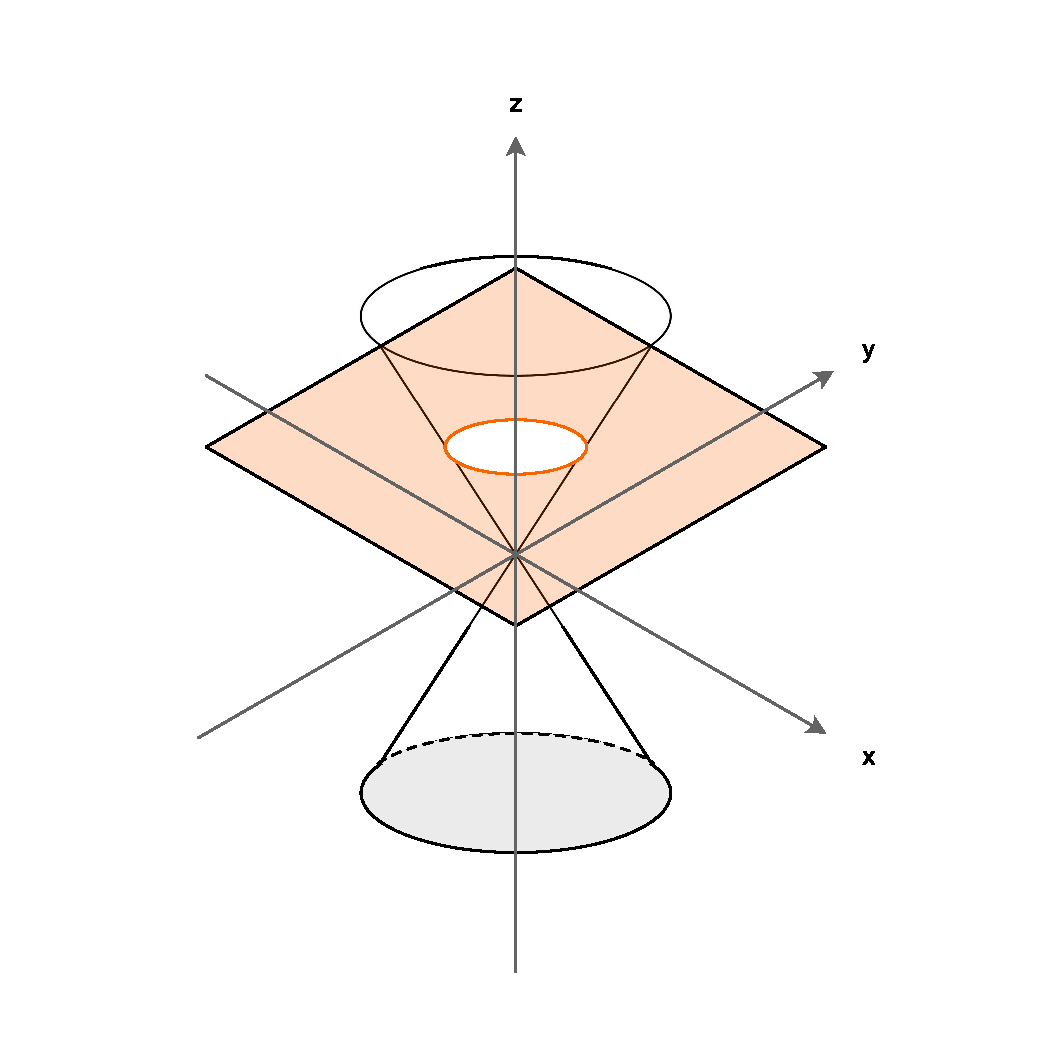
\includegraphics[width=8cm]{grafiken/kegelschnitte/kreis}
	\begin{tikzpicture}
		\begin{axis}[
				defaultnonumbers,
				xmin=-1.2, xmax=1.2,
				ymin=-1.2, ymax=1.2,
				width=8cm
			]
			\draw (0,0) ellipse [x radius=1cm, y radius=1cm];
		\end{axis}
	\end{tikzpicture}
	\caption{Kegelschnitt: Kreis}
\end{figure}

\paragraph{Einheitskreis}

\[
	A = B = 1 \quad E = -1 \quad x^2 + y^2 = 1
\]

\paragraph{Hauptform vom Kreis}

\[
	{(x - x_0)}^2 + {(y - y_0)}^2 = r^2
\]


\subsubsection{Ellipse}

\[
	A \cdot B > 0, A \neq B
\]

\begin{figure}[H]
	\centering
	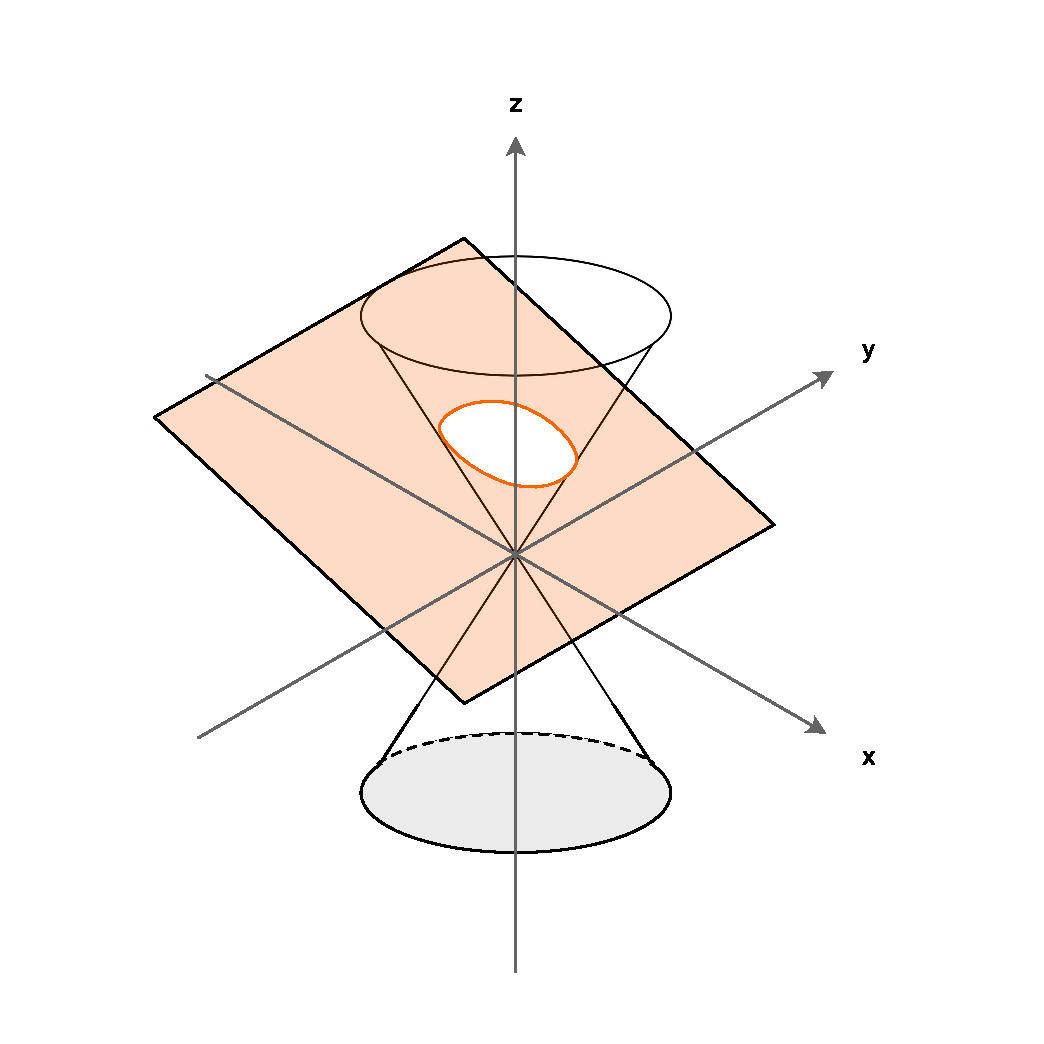
\includegraphics[width=8cm]{grafiken/kegelschnitte/ellipse}
	\begin{tikzpicture}
		\begin{axis}[
				defaultnonumbers,
				xmin=-2.2, xmax=2.2,
				ymin=-1.2, ymax=1.2,
				width=8cm
			]
			\draw (0,0) ellipse [x radius=2cm, y radius=1cm];
		\end{axis}
	\end{tikzpicture}
	\caption{Kegelschnitt: Ellipse}
\end{figure}

% \includegraphics{grafiken/Kegelschnitt_Ellipse}

\subsubsection{Hyperbel}

\[
	A \cdot B < 0, a \neq B
\]

\begin{figure}[H]
	\centering
	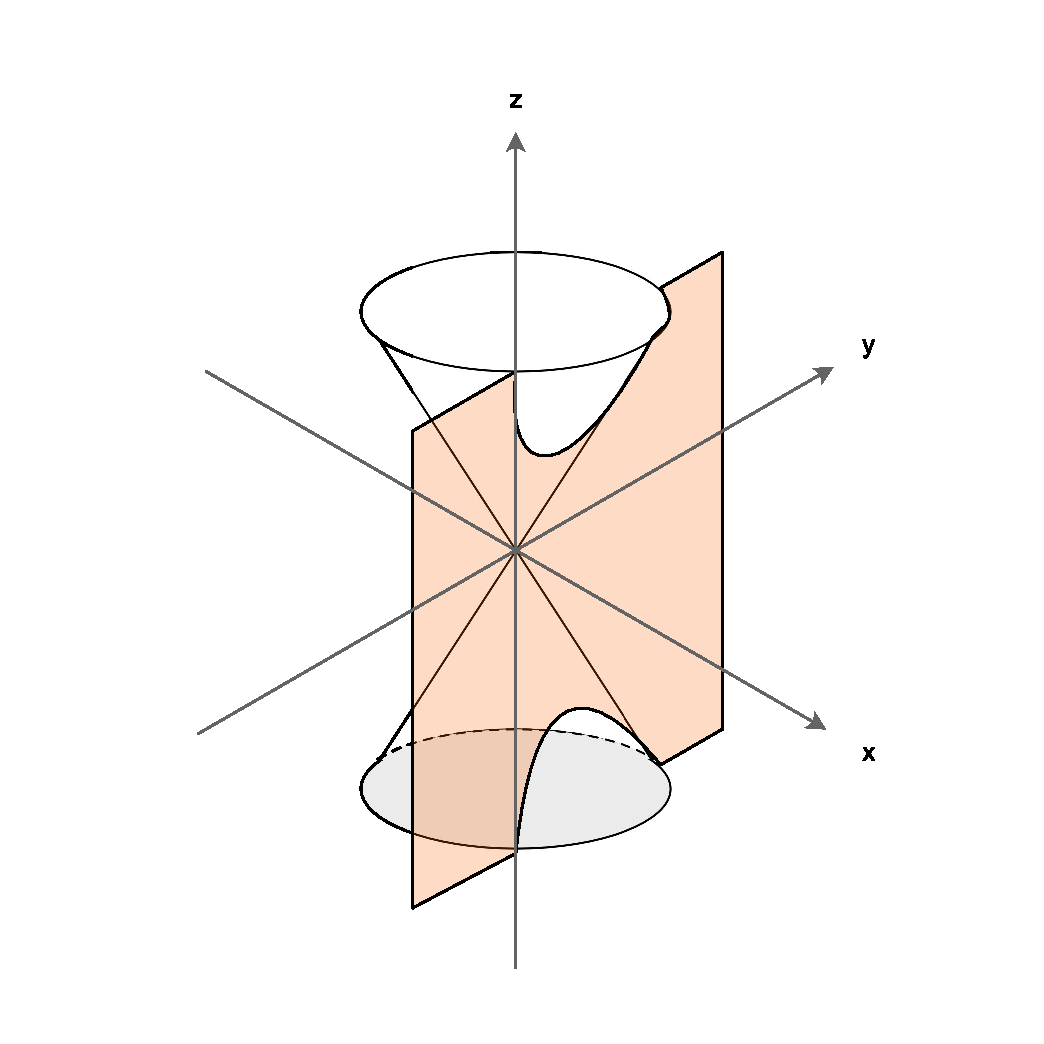
\includegraphics[width=8cm]{grafiken/kegelschnitte/hyperbel}
	\begin{tikzpicture}
		\begin{axis}[
				defaultnonumbers,
				xmin=-2.2, xmax=2.2,
				ymin=-2.2, ymax=2.2,
				width=8cm
			]
			\addplot [domain=-2:2] ({cosh(x)}, {sinh(x)});
			\addplot [domain=-2:2] ({-cosh(x)}, {sinh(x)});
		\end{axis}
	\end{tikzpicture}
	\caption{Kegelschnitt: Hyperbel}
\end{figure}

\subsubsection{Parabel}

\[
	(A = 0 \wedge B \neq 0) \vee (A \neq 0 \wedge B = 0)
\]

\begin{figure}[H]
	\centering
	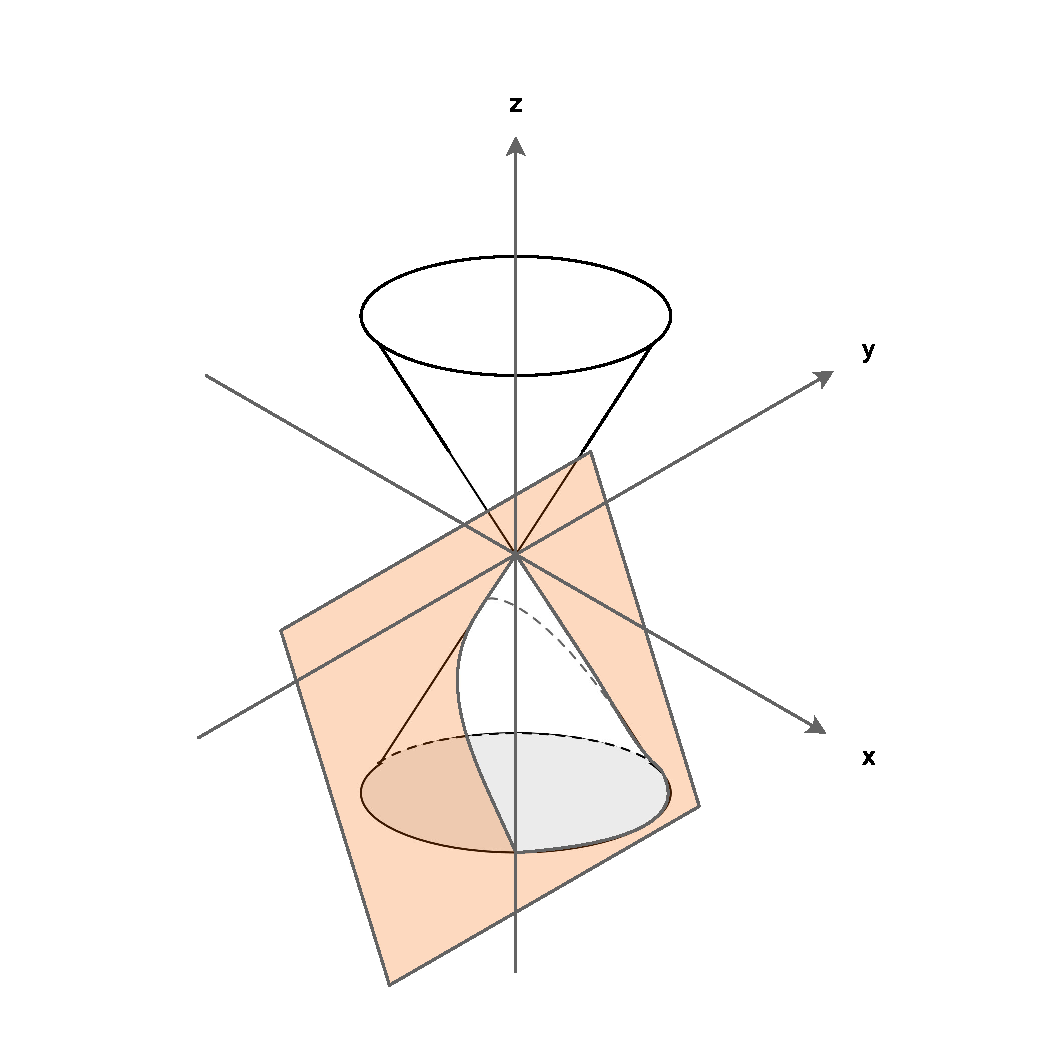
\includegraphics[width=8cm]{grafiken/kegelschnitte/parabel}
	\begin{tikzpicture}
		\begin{axis}[
				defaultnonumbers,
				xmin=-2.2, xmax=2.2,
				ymin=-2.2, ymax=2.2,
				width=8cm
			]
			\addplot [domain=-2:2] {x^2};
		\end{axis}
	\end{tikzpicture}
	\caption{Kegelschnitt: Parabel}
\end{figure}

\subsection{Exponentialfunktionen}

\paragraph{Allgemeine Form}

\[
	y = a^x \quad a \neq 1
\]

\begin{center}
	\( a > 0 \) damit wir in \( \mathbb{R} \) bleiben

	\( a \) wird Basis genannt, \( x \) Exponent

	\( a > 1 \) monoton steigend

	\( a < 1 \) monoton fallend
\end{center}

\begin{figure}[H]
	\centering
	\begin{tikzpicture}
		\begin{axis}[
				defaultnonumbers,
				xmin=-2.2, xmax=2.2,
				ymin=-1.2, ymax=3.2,
				width=8cm
			]
			\addplot[orange, smooth, samples=100, domain=-4:4] {e^x};
			\addplot[cyan, smooth, samples=100, domain=-4:4] {e^-x};
			\node [right] at (axis cs: 1.2, 3) {\( a > 1 \)};
			\node [left] at (axis cs: -1.2, 3) {\( a < 1 \)};
		\end{axis}
	\end{tikzpicture}
	\caption{exponentiell steigend (\( e^x \)) und fallend (\( e^{-x} \))}
\end{figure}

\begin{figure}[H]
	\centering
	\begin{align*}
		y(t)        & = {(1 + \omega)}^{t} \cdot y_0                            \\
		\Delta y(t) & \sim y(t-1)                                               \\
		\Delta y(t) & = \omega \cdot y(t-1) \quad \omega : \text{Wachstumsrate}
	\end{align*}
	\begin{tikzpicture}
		\begin{axis}[
				default,
				xmin=-1.2, xmax=6.2,
				ymin=-0.2, ymax=5.2,
				width=10cm,
				height=12cm,
				yticklabels={},
				xlabel={t},
			]
			\addplot [orange, smooth, samples=100, domain=-4:4] {e^(0.5*x)};

			\node [left] at (axis cs: -0.2, 1.0000) {\( y(0) \)};
			\node [left] at (axis cs: -0.2, 1.6487) {\( y(1) \)};
			\node [left] at (axis cs: -0.2, 2.7183) {\( y(2) \)};
			\node [left] at (axis cs: -0.2, 4.4817) {\( y(3) \)};

			\draw [dotted, thick] (-0.2, 1.0000) -- (6.2, 1);
			\draw [dotted, thick] (-0.2, 1.6487) -- (6.2, 1.6487);
			\draw [dotted, thick] (-0.2, 2.7183) -- (6.2, 2.7183);
			\draw [dotted, thick] (-0.2, 4.4817) -- (6.2, 4.4817);

			\draw [decorate,decoration={brace,amplitude=4pt}] (1, 1.6487) -- (1, 1);
			\draw [decorate,decoration={brace,amplitude=4pt}] (2, 2.7183) -- (2, 1.6487);
			\draw [decorate,decoration={brace,amplitude=4pt}] (3, 4.4817) -- (3, 2.7183);

			\node [right] at (axis cs: 1.2, 1.3244) {\( \Delta y(1) = \omega \cdot y(0) \)};
			\node [right] at (axis cs: 2.2, 2.1835) {\( \Delta y(2) = \omega \cdot y(1) \)};
			\node [right] at (axis cs: 3.2, 3.6000) {\( \Delta y(3) = \omega \cdot y(2) \)};
		\end{axis}
	\end{tikzpicture}
	\[
		\begin{alignedat}{5}
			\Delta y(3) &= y(3) - y(2) &= \omega \cdot y(2) \quad
			&\Rightarrow y(3) &= y(2) \cdot (1 + \omega) &= y(0) \cdot {(1+\omega)}^3 \\
			\Delta y(2) &= y(2) - y(1) &= \omega \cdot y(1) \quad
			&\Rightarrow y(2) &= y(1) \cdot (1 + \omega) &= y(0) \cdot {(1+\omega)}^2 \\
			\Delta y(1) &= y(1) - y(0) &= \omega \cdot y(0) \quad
			&\Rightarrow y(1) &= y(0) \cdot (1 + \omega) &= y(0) \cdot (1+\omega)
		\end{alignedat}
	\]
	% \caption{}
\end{figure}

\begin{uebung}[1]
	\begin{equation*}
		\begin{array}{lrl}
			                & 9^{x-1}       & = 27          \\
			\Leftrightarrow & 9^{x-1}       & = 3^3         \\
			\Leftrightarrow & {(3^2)}^{x-1} & = 3^3         \\
			\Leftrightarrow & 3^{2x-2}      & = 3^3         \\
			\Rightarrow     & 2x-2          & = 3           \\
			\Leftrightarrow & 2x            & = 5           \\
			\Leftrightarrow & x             & = \frac{5}{2}
		\end{array}
	\end{equation*}
\end{uebung}

\begin{uebung}[2]
	\begin{equation*}
		\begin{array}{lrl}
			                & {\left(\frac{4}{9}\right)}^{x-2}                    & = \frac{8}{27} \\
			\Leftrightarrow & {\left(\frac{4}{9}\right)}^{x-2}                    & =
			{\left(\frac{2}{3}\right)}^{3}                                                         \\
			\Leftrightarrow & {\left({\left(\frac{2}{3}\right)}^{2}\right)}^{x-2} & =
			{\left(\frac{2}{3}\right)}^{3}                                                         \\
			\Leftrightarrow & {\left(\frac{2}{3}\right)}^{2x-4}                   & =
			{\left(\frac{2}{3}\right)}^{3}                                                         \\
			\Rightarrow     & 2x-4                                                & = 3            \\
			\Leftrightarrow & 2x                                                  & = 7            \\
			\Leftrightarrow & x                                                   & = \frac{7}{2}
		\end{array}
	\end{equation*}
\end{uebung}

\begin{uebung}[3]
	\begin{equation*}
		\begin{array}{lrlr}
			                & 8 \cdot 9^{x-3} + 4^{x-3}     & = 3^{2x-4}                                    &                            \\
			\Leftrightarrow & 8 \cdot 3^{2x-9} + 4^{x-3}    & = 3^{2x-4}                                    &                            \\
			\Leftrightarrow & 2^3 \cdot 3^{2x-9} + 2^{2x-6} & = 3^{2x-4}                                    & \mid -(2^3 \cdot 3^{2x-9}) \\
			\Leftrightarrow & 2^{2x-6}                      & = 3^{2x-4} - 2^3 \cdot 3^{2x-9}               &                            \\
			\Leftrightarrow & 2^{2x-6}                      & = 3^{2} \cdot 3^{2x-6} - 2^{3} \cdot 3^{2x-9}                              \\
			\Leftrightarrow & 2^{2x-6}                      & = (3^2 - 2^3)
			% TODO: siehe Zettel - ergänzen 
		\end{array}
	\end{equation*}
\end{uebung}

\subsection{Logarithmusfunktionen}

Die Lösung \( x \) der Gleichung \( a^x = b \) nennt man
den Logarithmus von \( b \) zur Basis \( a \):

\[
    x = \log_a(b)
\]

Der Logarithmus von \( b \) zur Basis \( a \) ist jene reelle
Zahl \( x \) mit der man \( a \) potenzieren muss, um \( b \)
zu erhalten:

\[
    a^{\log_a(b)} = b    
\]

Die Logarithmusfunktion ist damit die Umkehrfunktion zur
Exponentialfunktion.


\begin{figure}[H]
    \centering
    \begin{tikzpicture}
        \begin{axis}[
                default,
                xmin=-2.2, xmax=2.2,
                ymin=-1.2, ymax=3.2,
                width=8cm
            ]
            \addplot[orange, smooth, samples=100, domain=0:2.2] {ln(x)};
            \addplot[cyan, smooth, samples=100, domain=0:2.2] {-ln(x)};
        \end{axis}
    \end{tikzpicture}
    \caption{Logarithmus steigend (\( \ln(x) \)) und fallend (\( -\ln{x} \))}
\end{figure}


\paragraph{Basis:}
\begin{equation*}
    \begin{array}{lll}
        a = e &\Rightarrow \log_e(x) &= \ln(x) \\
        a = 2 &\Rightarrow \log_2(x) &= \ld(x) = \lb(x) \\
        a = 10 &\Rightarrow \log_{10}(x) &= \lg(x)
    \end{array}
\end{equation*}

\subsubsection{Rechenregeln}

\begin{align*}
    \ln(a \cdot b) &= \ln(e^{\alpha} \cdot e^{\beta}) \\
    &= \ln(e^{(\alpha + \beta)}) \\
    &= \alpha + \beta \\
    &= \ln(e^{\alpha}) + \ln(e^{\beta}) \\
    &= \ln(a) + \ln (b) \\
    \\
    \ln(a^3) &= \ln(a^2 \cdot a) \\
    &= \ln(a^2) + \ln(a) \\
    &= \ln(a) + \ln(a) + \ln(a) \\
    &= 3 \cdot \ln(a) \\
    \\
    \ln(a^n) &= n \cdot \ln(a) \\
    \\
    \ln(\frac{a}{b}) &= \ln(a) + \ln(b^{-1}) \\
    &= \ln(a) - \ln(b)
\end{align*}

\subsubsection{Basiswechsel}
\[
    \log_a(x) \rightarrow \log_b(x)    
\]

\begin{align*}
    \log_a(x) = \log_a\left(b^{\log_b(x)}\right)
    &= \log_b(x) \cdot \log_a(b) \\
    \Rightarrow \log_a(x) &= \log_b(x) \cdot \frac{1}{\log_b(a)} \\
    \Rightarrow \log_a(x) &= \frac{\log_b(x)}{\log_b(a)} \\
    \text{wenn \(x = a\):} \\
    \log_a(a) &= \log_b(a) \cdot \log_a(b) = 1 \\
    \Rightarrow \log_a(b) &= \frac{1}{\log_b(a)} \\
    \\
    \text{Beispiel:} \\
    \log_3(5) &= \frac{\ln(5)}{\ln(3)}
\end{align*}

\paragraph{Beispiele}

\begin{align*}
    & \log(2) - \log(a) + \frac{1}{2} \log(b) \\
    &= \log\left(\frac{2}{a}\right) + \log\left(b^{\frac{1}{2}}\right) \\
    &= \log\left(\frac{2}{a}\right) + \log\left(\sqrt{b}\right) \\
    &= \log\left(\frac{2 \sqrt{b}}{a}\right)
\end{align*}

\begin{align*}
    \log(1-x) + \log(1+x) - 2 \log(x) \\
    &= \log((1-x)(1+x)) - \log\left(x^2\right) \\
    &= \log(1-x^2) - \log\left(x^2\right) \\
    &= \log\left(\frac{1-x^2}{x^2}\right) = \log\left(\frac{1}{x^2}-1\right)
\end{align*}

\begin{align*}
    10^x &= 2 \\
    \lg\left(10^x\right) &= \lg(2) \\
    x \lg(10) &= \lg(2) \\
    x \cdot 1 &= \lg(2) \\
    x &= \lg(2)
\end{align*}

\subsection{Stetigkeit und Grenzwert von Funktionen}

\[
	\lim_{x \rightarrow x_0} f(x) = g
\]

\( f(x) \) hat an der Stelle \( x_0 \) den Grenzwert \( g \),
wenn es zu einem beliebig kleinen \( \epsilon > 0 \) eine Zahl \( \delta(\epsilon) \)
gibt, so dass \( \mid f(x) - g \mid < \epsilon \) ist,
\( \forall x \) für die \( \mid x - x_0 \mid < \delta \) gibt.

\begin{figure}[H]
	\centering
	\begin{tikzpicture}
		\begin{axis}[
				default,
				xmin=-2.5, xmax=3.5,
				ymin=-0.5, ymax=3.5,
				width=8cm,
				xticklabels={},
				yticklabels={}
			]
			\addplot[orange, smooth, samples=100, domain=-4:4] {1.5^x};

			\draw [dotted, thick] (1, -0.2) -- (1, 1.5);
			\draw [dotted, thick] (2, -0.2) -- (2, 2.25);
			\draw [dotted, thick] (3, -0.2) -- (3, 3.375);

			\draw [dotted, thick] (-0.2, 1.5) -- (1, 1.5);
			\draw [dotted, thick] (-0.2, 2.25) -- (2, 2.25);
			\draw [dotted, thick] (-0.2, 3.375) -- (3, 3.375);

			\node at (axis cs: 1, -0.3) {\( x_0 - \delta \)};
			\node at (axis cs: 2, -0.3) {\( x_0 \)};
			\node at (axis cs: 3, -0.3) {\( x_0 + \delta \)};

			\node[left] at (axis cs: -0.2, 1.5) {\( y_0 - \epsilon \)};
			\node[left] at (axis cs: -0.2, 2.25) {\( f(x_0) = y_0 \)};
			\node[left] at (axis cs: -0.2, 3.375) {\( y_0 + \epsilon \)};
		\end{axis}
	\end{tikzpicture}
	\caption{}
\end{figure}

\subsubsection{Definitionslücke}

\paragraph{Beispiel}

\[
	y = \frac{x^2 - 1}{x - 1}
\]

\begin{figure}[H]
	\centering
	\begin{tikzpicture}
		\begin{axis}[
				default,
				xmin=-0.5, xmax=3.5,
				ymin=-0.5, ymax=3.5,
				width=8cm
			]
			\addplot[orange, smooth, samples=100, domain=-4:4] {(x^2 - 1) / (x - 1)};
			\addplot[mark=o] coordinates {(1,2)};
			\node[right] at (axis cs: 1, 2) {Definitionslücke};
		\end{axis}
	\end{tikzpicture}
	\caption{\(\frac{x^2 - 1}{x - 1}\)}
\end{figure}

\[
	\lim_{x \rightarrow 1} \frac{x^2 - 1^2}{x - 1}
	= \lim_{x \rightarrow 1} \frac{(x - 1)(x + 1)}{x - 1}
	= \lim_{x \rightarrow 1} (x+1)
	= 2
\]

\textbf{rechtseitiger Grenzwert}

\[
	x > x_0: \lim_{x \rightarrow x_0} f(x) = 2 = g_{+}
\]

\textbf{rechtseitiger Grenzwert}

\[
	x < x_0: \lim_{x \rightarrow x_0} f(x) = 2 = g_{-}
\]


\[
	g_{+} = g_{-} \Rightarrow \text{\(f(x_0)\) ist nicht definiert}
\]

\subsubsection{Sprungstelle}

\begin{figure}[H]
	\centering
	\begin{tikzpicture}
		\begin{axis}[
				default,
				xmin=-0.5, xmax=3.5,
				ymin=-0.5, ymax=3.5,
				width=8cm,
				xticklabels={},
				yticklabels={}
			]
			\addplot[color1, smooth, samples=100, domain=-4:2] {2^x - 2};
			\addplot[color1, smooth, samples=100, domain=2:4] {-(x - 2)^2 + 3};

			\draw [dotted, thick] (2, -0.2) -- (2, 3.2);
			\node at (axis cs: 2, -0.3) {Sprungstelle};
		\end{axis}
	\end{tikzpicture}
	\caption{Funktion mit Sprungstelle}
\end{figure}

\[
	f(x) =
	\begin{cases}
		2^x - 2          & \quad x \leq 2 \\
		-{(x - 2)}^2 + 3 & \quad x > 2
	\end{cases}
\]

\[
	g_{+} \neq g_{-} \Rightarrow \text{Sprungstelle}
\]

\subsubsection{Polstelle}

\begin{figure}[H]
	\centering
	\begin{tikzpicture}
		\begin{axis}[
				default,
				xmin=-2.5, xmax=2.5,
				ymin=-2.5, ymax=2.5,
				width=8cm
			]
			\addplot[color1, smooth, samples=100, domain=-4:-0.1] {1/x};
			\addplot[color1, smooth, samples=100, domain=0.1:4] {1/x};
		\end{axis}
	\end{tikzpicture}
	\caption{\(y = \frac{1}{x}\)}
\end{figure}

\begin{align*}
	\begin{rcases}
		\lim_{x \rightarrow 0_+} f(x) &= \infty \\
		\lim_{x \rightarrow 0_-} f(x) &= -\infty
	\end{rcases}
	f(x), g\; \text{existieren nicht}
\end{align*}



\section{Differentialrechnung}

\subsection{Einleitung}

\begin{figure}[H]
	\centering
	\begin{tikzpicture}
		\begin{axis}[
				default,
				xmin=-0.5, xmax=4.5,
				ymin=-0.5, ymax=4.5,
				width=10cm,
				xticklabels={},
				yticklabels={}
			]
			\addplot[orange, thick, smooth, samples=100, domain=-1:5] {-(0.5 * x - 2)^2 + 4};
			\addplot[mark=x] coordinates {(1, 1.75)};
			\addplot[mark=x] coordinates {(3, 3.75)};

			\draw[dotted, thick] (1, -0.2) -- (1, 1.75);
			\draw[dotted, thick] (3, -0.2) -- (3, 3.75);
			\draw[dotted, thick] (-0.2, 1.75) -- (1, 1.75);
			\draw[dotted, thick] (-0.2, 3.75) -- (3, 3.75);

			\node[below] at (axis cs: 1, -0.2) {\(x_0\)};
			\node[below] at (axis cs: 3, -0.2) {\(x_1\)};
			\node[left] at (axis cs: -0.2, 1.75) {\(y_0\)};
			\node[left] at (axis cs: -0.2, 3.75) {\(y_1\)};

			\draw[->] (1.5, 1.75) arc (0 : 58 : 0.4);
			\node[above right] at (axis cs: 1.15, 1.75) {\(\alpha\)};

			\draw (1, 1.75) -- (3, 1.75);
			\draw (3, 1.75) -- (3, 3.75);
			\draw[mkblue, thick] (0.5, 1.25) -- (3.5, 4.25);
			\node[mkblue, left] at (axis cs: 3, 4) {Sekante};
			\addplot[mkgreen, thick, smooth, samples=100, domain=0.5:2.2] {1.5*x+0.25};
			\node[mkgreen, left] at (axis cs: 2, 3.25) {Tangente in \(P_0\)};

			\node[below right] at (axis cs: 1, 1.75) {\(P_0\)};
			\node[below right] at (axis cs: 3, 3.75) {\(P_1\)};
			\node[below] at (axis cs: 2, 1.75) {\(\Delta x\)};
			\node[right] at (axis cs: 3, 2.75) {\(\Delta y\)};
		\end{axis}
	\end{tikzpicture}
	\caption{Graphische Herleitung des Differenzenquotient}
\end{figure}

\paragraph{Differenzenquotient}

\[
	\tan \alpha = \frac{\Delta y}{\Delta x} = \frac{y_1 - y_0}{x_1 - x_0}
\]

\paragraph{Differentialquotient}

\[
	\lim_{x_1 \rightarrow x_0} \frac{y_1 - y_0}{x_1 - x_0} = \tan \alpha_0
\]

\paragraph{1. Ableitung von \(f(x) \entspricht f'(x_0)\)}

\[
	\lim_{x_1 \rightarrow x_0} \frac{y_1 - y_0}{x_1 - x_0}= y'(x_0)
\]

\begin{align*}
	x_1 - x_0       & = \Delta x                                                                  \\
	\Rightarrow x_1 & = \Delta x + x_0                                                            \\
	\Rightarrow \lim_{x_1 \rightarrow x_0} \frac{y(x_1) + y(x_0)}{x_1 - x_0}
	                & = \lim_{\Delta x \rightarrow 0} \frac{y(x_0 + \Delta x) - y(x_0)}{\Delta x}
\end{align*}

\paragraph{Ableitungsfolge}

\[
	\begin{array}{ccccccccccc}
		 & \frac{\diff}{\diff x} &
		 & \frac{\diff}{\diff x} &
		 & \frac{\diff}{\diff x} &
		 & \frac{\diff}{\diff x} &                             \\
		y(x)
		 & \rightarrow           & y'(x)
		 & \rightarrow           & y''(x)
		 & \rightarrow           & y'''(x)
		 & \rightarrow           & y^{(4)}(x)
		 & \cdots                                              \\
		 &                       & \frac{\diff y}{\diff x}
		 &                       & \frac{\diff^2 y}{\diff x^2}
		 &                       & \frac{\diff^3 y}{\diff x^3}
		 &                       & \frac{\diff^4 y}{\diff x^4}
	\end{array}
\]

\paragraph{Beispiele}

\subparagraph{Ableitung von Polynomfunktionen}

\begin{align*}
	y  & = f(x) = x \quad y_1 = y(x_1) = x_1;\ y_2 = y(x_2) = x_2                                                                                                               \\
	y' & = \lim_{x_1 \rightarrow x_0} \frac{y_1 - y_0}{x_1 - x_0}                                                                                                               \\
	   & = \lim_{x_1 \rightarrow x_0} \frac{x_1 - x_0}{x_1 - x_0} = 1                                                                                                           \\
	\\
	y  & = f(x) = x^2                                                                                                                                                           \\
	y' & = \lim_{x_1 \rightarrow x_0} \frac{y_1 - y_0}{x_1 - x_0}                                                                                                               \\
	   & = \lim_{x_1 \rightarrow x_0} \frac{x_1^2 - x_0^2}{x_1 - x_0}                                                                                                           \\
	   & = \lim_{x_1 \rightarrow x_0} \frac{(x_1 - x_2)(x_1 + x_0)}{x_1 - x_0}                                                                                                  \\
	   & = \lim_{x_1 \rightarrow x_0} (x_1 + x_0) = 2x                                                                                                                          \\
	\\
	y  & = f(x) = x^n                                                                                                                                                           \\
	y' & = \lim_{x_1 \rightarrow x_0} \frac{x_1^n - x_0^n}{x_1 - x_0}                                                                          &  & \mid \text{Polynomdivision} \\
	   & = \lim_{x_1 \rightarrow x_0} (x_0^0 \cdot x_1^{n-1} + x_0^1 \cdot x_1^{n-2} + x_0^2 \cdot x_2^{n-3} + \cdots + x_0^{n-1} \cdot x_1^0)                                  \\
	   & = n \cdot x^{n-1}
\end{align*}

\subparagraph{Ableitung von Logarithmusfunktionen}

\begin{align*}
	y              & = f(x) = \log_a x                                                                                                                                               \\
	y'(x_0)        & = \lim_{\Delta x \rightarrow 0} \frac{\log_a(x_0 + \Delta x) - \log_a(x_0)}{\Delta x}                                                                           \\
	               & = \lim_{\Delta x \rightarrow 0} \frac{\log_a \left( \frac{x_0 + \Delta x}{x_0} \right)}{\Delta x} &  & \mid \Delta x = \frac{x_0}{n}                            \\
	\Rightarrow    & = \limtoinfty{n} \frac{\log_a \left( \frac{x_0 + \frac{x_0}{n}} {x_0} \right)}{\frac{x_0}{n}}                                                                   \\
	               & = \limtoinfty{n} n \cdot \frac{\log_a \left( 1 + \frac{1}{n} \right)}{x_0}                                                                                      \\
	               & = \frac{1}{x_0} \limtoinfty{n} \log_a {\left( 1 + \frac{1}{n} \right)}^{n}                                                                                      \\
	               & = \frac{1}{x_0} \log_a \left( \limtoinfty{n} {\left( 1 + \frac{1}{n} \right)}^n \right)           &  & \mid \text{Siehe Rechnung~\ref{eq:euler}}                \\
	\Rightarrow y' & = \frac{1}{x} \cdot \log_a \e = \frac{1}{x \cdot \ln a}                                           &  & \mid \log_a \e = \frac{1}{\log_{\e} a} = \frac{1}{\ln a} \\
	\\
	y              & = f(x) = \ln x = \log_{\e} x                                                                                                                                    \\
	y'             & = \frac{1}{x} \log_{\e} e = \frac{1}{x}
\end{align*}


\paragraph{Annäherung an die eulersche Zahl \( \e \)}
\begin{align}
	\begin{split}
		\label{eq:euler}
		\limtoinfty{n} a_n = \limtoinfty{n} {\left( 1 + \frac{1}{n} \right)}^n = e &\approx 2.718\dots \\
		a_n = {\left( 1 + \frac{1}{n} \right)}^n
		\Rightarrow a_1 &= 2 \\
		a_2 &= 2,25 \\
		a_3 &= 2,7 \\
		\vdots
	\end{split}
\end{align}

\subsection{Ableitungsregeln}

\begin{enumerate}
    \item Konstantenregel
        \begin{align*}
			y(x) &= c \\
			y'(x) &= 0
        \end{align*}
    \item Faktorregel
        \begin{align*}
			y(x) &= c \cdot u(x) \\
			y'(x) &= c \cdot u'(x)
        \end{align*}
    \item Summenregel
    	\begin{align*}
			y(x) &= u(x) + v(x) \\
			y'(x) &= u'(x) + v'(x)
		\end{align*}
    \item Produktregel
		\begin{align*}
            y(x) &= u(x) \cdot v(x) \\
            y'(x) &= u(x) \cdot v'(x) + u'(x) \cdot v(x)
        \end{align*}
    \item Quotientenregel
        \begin{align*}
            y(x) &= \dfrac{u(x)}{v(x)} \\
            y'(x) &= \dfrac{v(x) \cdot u'(x) - v'(x) \cdot u(x)}{v^2(x)}
        \end{align*}
    \item Kettenregel
        \begin{align*}
            y(x) &= f(\phi(x)) = f(z),\ z = \phi(x) \\
            y'(x) &= \dfrac{\diff y}{\diff x} = \underbrace{\dfrac{\diff f}{\diff z}}_{\text{äußere Abl.}} \cdot \underbrace{\dfrac{\diff \phi}{\diff x}}_{\text{innere Abl.}}
        \end{align*}
    \item Ableitung der Umkehrfunktion
        \begin{align*}
            f(x) &= y,\ x = f^{-1}(f(x)) \\
            f'(x) &= \dfrac{1}{\dfrac{\diff f}{\diff x}}
        \end{align*}
    \item Logarithmisches Differenzieren
        \begin{align*}
            y(x) &= u{(x)}^{v(x)} \\
            &\text{I.\, logarithmiere} \\
            &\text{II.\, differenzieren mit Regel 1--7}
        \end{align*}
\end{enumerate}

% TODO: Herleitung einzelner Regeln
% TODO: Übungsaufgaben
\subsection{Differenzieren Trigonometrischer Funktionen}

\begin{figure}[H]
	\centering
	\begin{tikzpicture}
		\node at (0,0) {\( \sin(x) \)};
		\node[right] at (2,-2) {\( \cos(x) \)};
		\node at (0,-4) {\( -\sin(x) \)};
		\node[left] at (-2,-2) {\( -\cos(x) \)};

		\draw[->, thick] (0.5,0.5) arc (-270: -360: 2);
		\draw[->, thick] (2.5,-2.5) arc (0: -90: 2);
		\draw[->, thick] (-0.5,-4.5) arc (-90: -180: 2);
		\draw[->, thick] (-2.5,-1.5) arc (-180: -270: 2);

		\node[] at (0,-2) {\( \frac{\diff}{\diff x} \)};
	\end{tikzpicture}
	\caption{Der Ableitungskreis für Sinus \& Cosinus}
\end{figure}

\subsubsection{Sinus}

\begin{align*}
	            & \limtozero{\Delta x} \frac{\sin(x_0 + \Delta x) - \sin(x_0)}{\Delta x}                                                                    \\
	            & = \limtozero{\Delta x} \frac{\sin(x_0) \cdot \cos(\Delta x) + \cos(x_0) \cdot \sin(\Delta x) - \sin(x_0)}{\Delta x}                       \\
	            & = \limtozero{\Delta x} \underbrace{\sin(x_0)}_{\text{A}} \underbrace{\frac{\cos(\Delta x) - 1}{\Delta x}}_{\text{B}} +
	\limtozero{\Delta x} \underbrace{\cos(x_0)}_{\text{A}} \underbrace{\frac{\sin(\Delta x)}{\Delta x}}_{\text{B}}                                          \\
	\\
	\text{A:\;} & \text{fester Wert}                                                                                                                        \\
	\text{B:\;} & \text{unbestimmter Ausdruck}                                                                                                              \\
	\\
	            & = \sin(x_0) \limtozero{\Delta x} \frac{\cos(\Delta x) - 1}{\Delta x} + \cos(x_0) \limtozero{\Delta x} \frac{\sin(\Delta x)}{\Delta x}     \\
	            & = \sin(x_0) \limtozero{\Delta x} \frac{(\cos(\Delta x) - 1) \cdot (\cos(\Delta x) + 1)}{\Delta x \cdot (\cos(\Delta x) + 1)} + \cdots     \\
	            & = \sin(x_0) \limtozero{\Delta x} \frac{\cos^2(\Delta x) - 1}{\Delta x \cdot (\cos(\Delta x) + 1)} + \cdots                                \\
	            & = \sin(x_0) \limtozero{\Delta x} \frac{- \sin^2(\Delta x) - 1}{\Delta x \cdot (\cos(\Delta x) + 1)} + \cdots                              \\
	            & = -\sin(x_0) \limtozero{\Delta x} \sin(\Delta x) \cdot \limtozero{\Delta x} \frac{\sin(\Delta x)}{\Delta x (\cos(\Delta x) + 1)} + \cdots \\
	            & = \text{usw.}
\end{align*}

\subsubsection{Cosinus}

\begin{align*}
	y  & = \cos(x)                                                                                                                 \\
	   & = \sin(x + \frac{\pi}{2}) = \sin(z),            &  & \mid z = x + \frac{\pi}{2}                                           \\
	   &                                                 &  & \mid \frac{\diff y}{\diff z} = \cos(z),\ \frac{\diff z}{\diff x} = 1 \\
	y' & = \cos\left(x + \frac{\pi}{2}\right) = -\sin(x)
\end{align*}

\subsubsection{Tangens}

\begin{align*}
	y  & = \tan(x) = \frac{\sin(x)}{\cos(x)}                          \\
	y' & = \frac{\cos(x)\cos(x) - \sin(x)\cdot (-\sin(x))}{\cos^2(x)} \\
	   & = \frac{\cos^2(x) + \sin^2(x)}{\cos^2(x)}                    \\
	   & = \frac{1}{\cos^2(x)} = 1 + \tan^2(x)
\end{align*}

\subsubsection{Cotangens}

\begin{align*}
	y  & = \cot(x) = {(\tan(x))}^{-1}                                    &  & \mid z = \tan(x)                                                                       \\
	   &                                                                 &  & \mid \frac{\diff z}{\diff x} = \frac{1}{\cos^2(x)},\ \frac{\diff y}{\diff z} = -z^{-2} \\
	y' & = \frac{1}{\cos^2(x)} \cdot \left( -\frac{1}{\tan^2(x)} \right)                                                                                             \\
	   & = -\frac{1}{\cos^2(x) \frac{\sin^2(x)}{\cos^2(x)}}                                                                                                          \\
	   & = -\frac{1}{\sin^2(x)} = -\left( 1 + \cot^2(x) \right)
\end{align*}

\subsubsection{Arkussinus}

\begin{align*}
	y       & = \arcsin(x)               &  & \mid \sin()                                                                                                                     \\
	\sin(y) & = \sin(\arcsin(x)) = x     &  & \mid \frac{\diff x}{\diff y} = \cos(y) \Rightarrow \frac{\diff y}{\diff x} = \frac{1}{\cos(y)} = \frac{1}{\sqrt{1 - \sin^2(y)}} \\
	y'      & = \frac{1}{\sqrt{1 - x^2}}
\end{align*}

\subsubsection{Arkuscosinus}

\begin{align*}
	y       & = \arccos(x)                &  & \mid \cos()                                                                                                                       \\
	\cos(y) & = x                         &  & \mid \frac{\diff x}{\diff y} = -\sin(y) \Rightarrow \frac{\diff y}{\diff x} = \frac{1}{-\sin(y)} = \frac{1}{\sqrt{1 - \cos^2(y)}} \\
	y'      & = -\frac{1}{\sqrt{1 - x^2}}
\end{align*}

\subsubsection{Arkustangens}

\begin{align*}
	y       & = \arctan(x)        &  & \mid \tan()                                                                                                \\
	\tan(y) & = x                 &  & \mid \frac{\diff x}{\diff y} = 1 + \tan^2(y) \Rightarrow \frac{\diff y}{\diff x} = \frac{1}{1 + \tan^2(y)} \\
	y'      & = \frac{1}{1 + x^2}
\end{align*}

\subsubsection{Arkuskotangens}

\begin{align*}
	y       & = \arccot(x)         &  & \mid \cot()                                                                                                 \\
	\cot(y) & = x                  &  & \mid \frac{\diff x}{\diff y} = 1 + \cot^2(y) \Rightarrow \frac{\diff y}{\diff x} = -\frac{1}{1 + \cot^2(y)} \\
	y'      & = -\frac{1}{1 + x^2}
\end{align*}


\subsection{Grenzwertregel von Bernoulli und de l’Hospital}

Für Grenzwerte, die auf einem unbestimmten Ausdruck der Form \enquote{\( \frac{0}{0} \)} oder \enquote{\( \frac{\infty}{\infty} \)} führen, gilt:

\[
	\limfromto{x}{x_0} \frac{f(x)}{g(x)} \overset{H}{=}
	\limfromto{x}{x_0} \frac{f'(x)}{g'(x)} =
	\limfromto{x}{x_0} \frac{f^{(k)}(x)}{g^{(k)}(x)}
	\quad k \geq 1,\ \text{minimal}
\]

weitere unbestimmte Ausdrücke:

\begin{description}[style=nextline]
	\item[\( 0 \cdot \infty,\ \infty \cdot 0 \)]
	      \( u \cdot v
	      \Rightarrow \cfrac{u}{\cfrac{1}{v}} \)
	\item[\( \infty - \infty \)]
	      \( u - v
	      \Rightarrow \cfrac{u \cdot v}{v} - \cfrac{v \cdot u}{u}
	      \Rightarrow \cfrac{\cfrac{1}{v}}{\cfrac{1}{u\ v}} - \cfrac{\cfrac{1}{u}}{\cfrac{1}{u\ v}} = \cfrac{\cfrac{1}{v}-\cfrac{1}{u}}{\cfrac{1}{u\ v}} \)
	\item[\( 0^0,\ \infty^0,\ 1^\infty \)]
	      \(
	      u^v \Rightarrow e^{v \cdot \ln(u)}
	      \)
\end{description}

\paragraph{Beispiel}

\subparagraph{1}

\begin{align*}
	y                               & = \frac{\sin(x)}{x}                                \\
	\limtozero{x} \frac{\sin(x)}{x} & \entspricht \frac{0}{0}                            \\
	\limtozero{x} \frac{\sin(x)}{x} & \overset{H}{=} \limtozero{x} \frac{\cos(x)}{1} = 1
\end{align*}

\subparagraph{2}

\begin{align*}
	 & \limtoinfty{x} {(1 + \frac{1}{x})}^x                                                                                           \\
	 & = \limtoinfty{x} e^{\ln {\left( 1 + \frac{1}{x} \right)}^x}                                                                    \\
	 & = \limtoinfty{x} e^{x \ln \left( 1 + \frac{1}{x} \right)}                                                                      \\
	 & = e^{\limtoinfty{x} \frac{\ln \left( 1 + \frac{1}{x} \right)}{\frac{1}{x}}}                                                    \\
	 & \overset{H}{=} e^{\limtoinfty{x} \frac{\frac{1}{\left(1 + \frac{1}{x}\right)} \left( -x^{-2} \right)}{\left( -x^{-2} \right)}} \\
	 & = e^{\limtoinfty{x} \frac{1}{1 + \frac{1}{x}}}                                                                                 \\
	 & = e^1 = e
\end{align*}

% TODO: Aufgaben S. 48
\subsection{Aufgabentypen zur Ableitung}

\subsubsection{Bestandteile der Kurvendiskussion}

\begin{enumerate}[I.]
	\item Definitionsbereich / Definitionslücke
	\item Symmetrie
	\item Nullstellen / \( f(0) \)
	\item Pole / vertikale Asymptote
	\item Ableitungen (i.\,d.\,R. bis 3.~Ordnung)
	\item reelle Extremwerte
	\item Wendepunkte
	\item Verhalten im Fernbereich
	\item Wertebereich
	\item Zeichnung
\end{enumerate}

\subsubsection{Extremwerte}

\begin{figure}[H]
	\centering
	\begin{tikzpicture}
		\begin{axis}[
				default,
				xmin=-0.5, xmax=3.5,
				ymin=-0.5, ymax=3.5,
				width=8cm,
				xticklabels={},
				yticklabels={}
			]
			\addplot[orange, smooth, samples=100, domain=-1:4] {(x-2)^3- 2 * x+6};

			\draw (0.7835034190722739, 3.0886621079036347) -- (1.583503419072274, 3.0886621079036347);
			\draw (2.4164965809277263, 0.9113378920963653) -- (3.2164965809277257, 0.9113378920963653);

			\draw[mkred, dotted, thick] (1.1835, -0.2) -- (1.1835, 4.2);
			\draw[mkred, dotted, thick] (2.8164, -0.2) -- (2.8164, 4.2);
		\end{axis}
	\end{tikzpicture}
	\qquad
	\begin{tikzpicture}
		\begin{axis}[
				default,
				xmin=-0.5, xmax=3.5,
				ymin=-0.5, ymax=3.5,
				width=8cm,
				xticklabels={},
				yticklabels={}
			]
			\addplot[orange, smooth, samples=100, domain=-1:4] {(x-1.5)^2 + 1.5};

			\draw (1.1, 1.5) -- (1.9, 1.5);

			\draw[mkred, dotted, thick] (1.5, -0.2) -- (1.5, 4.2);

		\end{axis}
	\end{tikzpicture}
	\caption{Funktionen mit Extremwerten}
\end{figure}

\paragraph{Notwendige Bedingung}

\[
	y'(x) = 0
\]

\paragraph{Hinreichende Bedingung}

\[
	y^{(k)}(x_E)
	\begin{cases}
		< 0\ \text{Maximum} \\
		> 0\ \text{Minimum}
	\end{cases}
	k \geq 2,\ \underbrace{\text{gerade, minimal}}_{\text{ungerade} \Rightarrow \text{Sattelpunkt}}
\]

\subsubsection{Wendepunkte}

\begin{figure}[H]
    \centering
    \begin{tikzpicture}
        \begin{axis}[
                default,
                xmin=-0.5, xmax=3.5,
                ymin=-0.5, ymax=3.5,
                width=8cm,
                xticklabels={},
                yticklabels={}
            ]
            \addplot[orange, smooth, samples=100, domain=-1:4] {(x-1.5)^3 + 2};
            
            \draw[mkred, dotted, thick] (1.5, -0.2) -- (1.5, 4.2);
        \end{axis}
    \end{tikzpicture}
    \qquad
    \begin{tikzpicture}
        \begin{axis}[
                default,
                xmin=-0.5, xmax=3.5,
                ymin=-0.5, ymax=3.5,
                width=8cm,
                xticklabels={},
                yticklabels={}
            ]
            \addplot[orange, smooth, samples=100, domain=-1:4] {-(x-1.5)^3 - 0.5*x + 2};
                        
            \draw[mkred, dotted, thick] (1.5, -0.2) -- (1.5, 4.2);
            
        \end{axis}
    \end{tikzpicture}
    \caption{Funktionen mit Wendestellen}
\end{figure}

\paragraph{Notwendige Bedingung}

\[
    y''(x_W) = 0
\]

\paragraph{Hinreichende Bedingung}

\[
    y^{(k)}(x_W) \neq 0 \quad k \geq 3,\ \text{ungerade, minimal}
\]

\subsubsection{Beispiel Kurvendiskussion}

\[
	y = f(x) = \frac{x^3 - 2x^2}{x^2 - x - 2} = x^2 \frac{x - 2}{x^2 - x - 2} = x^2 \frac{x - 2}{(x-2)(x+1)}
\]

\paragraph{Definitionsbereich}

\begin{align*}
	x^2 - x - 2 & = 0                                                        \\
	x_{P1,2}    & = \frac{1}{2} \pm \sqrt{\frac{1}{4} + \frac{8}{4}}         \\
	x_{P1}      & = -1,\quad x_{P2} = 2                                      \\
	D_f         & = \{ x \in \mathbb{R}\ |\ (x \neq -1) \wedge (x \neq 2) \}
\end{align*}

\subparagraph{Ersatzfunktionen}

\begin{align*}
	y* = x^2 \frac{\cancel{x - 2}}{\cancel{(x - 2)}(x + 1)} = \frac{x^2}{x + 1}
\end{align*}

\paragraph{Nullstellen}

\begin{align*}
	x_{N1,2} & = 0 \\
	x_{N3}   & = 2
\end{align*}

\paragraph{Verhalten im Fernbereich}

\begin{alignat*}{2}
	\limfromto{x}{-1_+} f(x) & = \frac{x^2}{x + 1} & = +\infty \\
	\limfromto{x}{-1_-} f(x) & = \frac{x^2}{x + 1} & = -\infty
\end{alignat*}

\paragraph{Asymptote}

\polyset{style=C, div=:,vars=x}
\polylongdiv{x^2}{x + 1}

\[
	y_A = x - 1 \qquad y^A = x - 1 + \frac{1}{x + 1}
\]

\paragraph{Ableitung}

\begin{align*}
	(y*)' & = \frac{(x + 1) 2x - x^2}{{(x + 1)}^2}
	= \frac{2x^2 + 2x - x^2}{{(x + 1)}^2}
	= \frac{x^2 + 2x}{{(x + 1)}^2}
	= x \frac{x + 2}{{(x + 1)}^2}
\end{align*}

\[
	\begin{array}{cccc}
		x_{E1} = 0  & y_{E1} = 0  & y_A''(x_{E1}) > 0 \Rightarrow \text{Minimum} \\
		x_{E2} = -2 & y_{E2} = -4 & y_A''(x_{E2}) < 0 \Rightarrow \text{Maximum}
	\end{array}
\]

\begin{align*}
	y^A     & = x - 1 + \frac{1}{x + 1}            \\
	(y^A)'  & = 1 - \frac{1}{{(x + 1)}^2}          \\
	        & = 1 - {(x + 1)}^{-2}                 \\
	(y^A)'' & = 2{(x + 1)}^{-3}                    \\
	        & = \frac{2}{{(x + 1)}^3}              \\
	        & \Rightarrow \text{Keine Wendestelle}
\end{align*}

\paragraph{Zeichnung}

\begin{figure}[H]
	\centering
	\begin{tikzpicture}
		\begin{axis}[
				default,
				xmin=-8.5, xmax=8.5,
				ymin=-8.5, ymax=8.5,
				width=12cm,
			]

			\addplot[color1, smooth, samples=100, domain=2.1:8] {(x^3 - 2*x^2)/(x^2 - x -2)};

			\addplot[color1, smooth, samples=100, domain=-1:1.9] {(x^3 - 2*x^2)/(x^2 - x -2)};

			\addplot[color1, smooth, samples=100, domain=-8:-1.1] {(x^3 - 2*x^2)/(x^2 - x -2)};

			\addplot[color3, dashed, smooth, samples=100, domain=-8:8] {x-1};

			\draw[color2, dotted, thick] (-1, -9) -- (-1, 9);

			\draw[color2, dotted, thick] (2, -9) -- (2, 9);
		\end{axis}
	\end{tikzpicture}
	\caption{Skizze}
\end{figure}

\subsubsection{Extremwertaufgabe}

\begin{figure}[H]
    \centering
    \begin{tikzpicture}
        \draw (1.5,0) arc [start angle=0,end angle=-180,x radius=1.5,y radius=1];
        \draw[dashed] (1.5,0) arc [start angle=0,end angle=180,x radius=1.5,y radius=1];
        
        \draw (0,3) ellipse (1.5cm and 1cm);
        \draw (-1.5,0) -- (-1.5,3);
        \draw (1.5,0) -- (1.5,3);
        
        \draw[dotted] (0,0) -- (0,3);
        \draw (0,3) -- (1.5,3);
        \node[above] at (0.75,3) {\( r \)};
        
        \draw (2,0) -- (2,3);
        \draw (1.9,0) -- (2.1,0);
        \draw (1.9,3) -- (2.1,3);
        \node[right] at (2,1.5) {\( h \)};
    \end{tikzpicture}
    \caption{Skizze Zylinder}
\end{figure}

gegeben: \( V \)

\( O, M \) soll minimal sein

\paragraph{Hauptbedingung}

\[
    O(r, h) = 2 \pi \cdot r^2 + h \cdot 2 \pi r    
\]

\paragraph{Nebenbedingung}

\[
    V = h \pi r^2 \Rightarrow h = \frac{V}{\pi r^2}
\]

\paragraph{Zielfunktion}

\begin{align*}
    O(r) &= 2 \pi r^2 + 2 \pi r \frac{V}{\pi r^2} \\
    &= 2 \pi r^2 + \frac{2V}{r} \\
    &= 2 \left(\pi r^2 + \frac{V}{r}\right)
\end{align*}

\begin{align*}
    \frac{\diff 0}{\diff r} &= 2 \left( 2 \pi r - \frac{V}{r^2} \right) \\
    \frac{\diff 0}{\diff r} (r=r_E) \overset{!}{=} \sigma &= 2 \left( 2 \pi r - \frac{V}{r^2} \right) \\
    2 \pi r &= \frac{V}{r^2} &\mid \cdot \frac{r^2}{V} \\
    r^3 &= \frac{V}{2 \pi} \\
    \Rightarrow r &= \sqrt[3]{\frac{V}{2 \pi}}
\end{align*}

\begin{align*}
    \frac{\diff 0}{\diff r} &= 2 \left( 2\pi + \frac{V}{r^3} \right) \\
    &= 2 \left( 2 \pi + \frac{V 2 \pi}{V}  \right) \\
    &= 2 (2 \pi + 2 \pi) \\
    &= 2 (4 \pi) \\
    &= 8 \pi > 0 \Rightarrow \text{Minimum}
\end{align*}

\begin{align*}
    h &= \frac{V}{\pi r^2} \text{ mit } r^2 = \frac{V}{2 \pi r} \\
    \Rightarrow h &= \frac{V}{\pi} \cdot \frac{2 \pi r}{V} = 2r
\end{align*}

\subsubsection{Produktionsfunktion}

\begin{figure}[H]
	\centering
	\begin{tikzpicture}
		\begin{axis}[
				defaultpure,
				xmin=-0.5, xmax=4.5,
				ymin=-1, ymax=8.5,
				width=8cm,
				xlabel={r}, ylabel={x},
				xticklabels={}, yticklabels={}
			]

			\addplot[color1, smooth, samples=100, domain=0:2] {0.5*x^3};
			\addplot[color1, smooth, samples=100, domain=2:5] {-(x-4)^2 + 8};
			\addplot[mkred, smooth, samples=100, domain=0:5] {(6.51)/(2.78) * x};


			\draw[dotted, thick] (2, 0) -- (2, 4);
			\draw[dotted, thick] (2.78, 0) -- (2.78, 6.51);
			\draw[dotted, thick] (4, 0) -- (4, 8);

			\node[below] at (2, 0) {\( r_W \)};
			\node[below] at (2.78, 0) {\( r_D* \)};
			\node[below] at (4, 0) {\( r* \)};
		\end{axis}
	\end{tikzpicture}
	\caption{Skizze Produktionsfunktion}
\end{figure}

\[
	x(r) = ar + br^2 - cr^3
\]

\begin{tabular}{l l}
	Output                          & \( x(r) \) maximal bei \( r* \)                                                                                                                                     \\
	Durchschnittsbetrag             & \( \bar{x}_D(r) = \frac{x(r)}{r} \) maximal bei \( r_{D}* \)                                                                                                        \\
	Grenzproduktivität, Grenzertrag & \( x'(r) = \frac{\diff x}{\diff y} \) maximal bei \( r_W \)                                                                                                         \\
	Elastizität                     & \( E(x, r) = \dfrac{\frac{\diff x}{x}}{\frac{\diff r}{r}} = \dfrac{\frac{\diff x}{\diff r}}{\frac{x}{r}} = \frac{\text{Grenzertrag}}{\text{Durchschnittsbetrag}} \)
\end{tabular}

\subsubsection{Kostenfunktion}

\begin{figure}[H]
    \centering
    \begin{tikzpicture}
        \begin{axis}[
            defaultpure,
            xmin=-0.5, xmax=3.5,
            ymin=-0.5, ymax=3.5,
            width=8cm,
            xlabel={x (Stück)}, ylabel={k},
            xticklabels={}, yticklabels={}
        ]

        \addplot[orange, smooth, samples=100, domain=0:8] {0.5*(x-1)^3 + 1.5};
        \addplot[mkred, smooth, samples=100, domain=0:5] {(1.86)/(1.89) * x};
        

        \draw[dotted, thick] (1, 0) -- (1, 4);
        \draw[dotted, thick] (1.86, 0) -- (1.86, 6.51);
        
        \node[below] at (1, 0) {\( x_W \)};
        \node[below] at (1.86, 0) {\( x_D* \)};
    \end{axis}
    \end{tikzpicture}
    \caption{Skizze Kostenfunktion}
\end{figure}

\begin{tabular}{l l}
    \( \overline{k_D} = \frac{k}{x} \) & Durchschnittskosten/Stück \\
    \( k' = \frac{\diff k}{\diff x} \) & Grenzkosten \\
    \( E(k,x) = \frac{k'}{\overline{k_D}} \)
\end{tabular}

\paragraph{Beispiel}

\begin{figure}[H]
    \centering
    \begin{tikzpicture}
        \begin{axis}[
            defaultpure,
            xmin=-100, xmax=2000,
            ymin=-100, ymax=100000,
            width=8cm,
            xlabel={p}, ylabel={x},
        ]

        \addplot[orange, smooth, samples=100, domain=0:25000] {-60*x+90000};
        

        \draw[dotted, thick] (1, 0) -- (1, 4);
        \draw[dotted, thick] (1.86, 0) -- (1.86, 6.51);
        
        \node[below] at (1, 0) {\( x_W \)};
        \node[below] at (1.86, 0) {\( x_D* \)};
    \end{axis}
    \end{tikzpicture}
    \caption{Skizze Beispiel}
\end{figure}

\begin{alignat*}{2}
    x(p) &= 90\,000-60p\quad &&1) p=500\\
    \frac{\diff x}{\diff p} &= -60 &&2) p=1000 \\
    x_1 &= 90\,000 - 60 \cdot 500 &&= 60\,000  \\
    x_2 &= 90\,000 - 60 \cdot 1000 &&= 30\,000 
\end{alignat*}

\begin{align*}
    E(x, p) &= \frac{\diff x}{\diff p} \cdot \frac{\diff p}{\diff x} \\
    E(x_1, p_1) &= -60 \cdot \frac{500}{60\,000} = -0,5 \\
    E(x_2, p_2) &= -60 \cdot \frac{1000}{30\,000} = -2
\end{align*}

\paragraph{Polypol \& Monopol}

\begin{figure}[H]
    \centering
    \begin{tikzpicture}
        \begin{axis}[
            defaultpure,
            xmin=-0.5, xmax=3.5,
            ymin=-0.5, ymax=3.5,
            width=8cm,
            xlabel={x}, ylabel={G, E, K},
            xticklabels={},
            yticklabels={}
        ]

        \addplot[name path=k, orange, smooth, samples=100, domain=0:4] {(x - 1.5)^3 + (x-2)^2 +1};
        \addplot[name path=e, mkred, smooth, samples=100, domain=0:4] {x};
        \addplot[mkblue, smooth, samples=100, domain=0:4] {1};
        
        \addplot fill between [of = k and e, split,
            every even segment/.style = {transparent},
            every odd segment/.style = {mkgreen!30}];

        \draw[dotted, thick] (1.38, 0) -- (1.38, 4);
        \draw[dotted, thick] (1.84, 0) -- (1.84, 4);
        \draw[dotted, thick] (2.58, 0) -- (2.58, 4);
        
        \node[below] at (1.38, 0) {\( G_S \)};
        \node[below] at (1.84, 0) {\( G_{Max} \)};
        \node[below] at (2.58, 0) {\( G_G \)};

        \node[above, mkblue] at (3, 1) {\( p(x) \)};
        \node[below, mkred] at (3, 3) {\( E \)};
        \node[above, orange] at (2.9, 3.2) {\( K \)};
    \end{axis}
    \end{tikzpicture}
    \quad
    \begin{tikzpicture}
        \begin{axis}[
            defaultpure,
            xmin=-0.5, xmax=3.5,
            ymin=-0.5, ymax=3.5,
            width=8cm,
            xlabel={x}, ylabel={G, E, K},
            xticklabels={},
            yticklabels={}
        ]

        \addplot[name path=k, orange, smooth, samples=100, domain=0:4] {(x - 1.5)^3 + (x-2)^2 +1};
        \addplot[name path=e, mkred, smooth, samples=100, domain=0:4] {-(x - 1.4)^2 + 2};
        \addplot[mkblue, smooth, samples=100, domain=0:4] {-(2.2 / 2.81) * x + 2.2};
        
        \addplot fill between [of = k and e, split,
            every even segment/.style = {transparent},
            every odd segment/.style = {mkgreen!30}];

        \draw[dotted, thick] (1.02, 0) -- (1.02, 4);
        \draw[dotted, thick] (1.6, 0) -- (1.6, 4);
        \draw[dotted, thick] (2.19, 0) -- (2.19, 4);
        
        \node[below] at (1.02, 0) {\( G_S \)};
        \node[below] at (1.6, 0) {\( G_{Max} \)};
        \node[below] at (2.19, 0) {\( G_G \)};
        \node[below] at (2.8, 0) {\( \frac{P}{P_G} \)};
        
        \node[below, left] at (1.6, 0.9) {\( P_{opt} \)};
        \draw (1.5, 0.85) -- (1.7, 1.05);
        \draw (1.7, 0.85) -- (1.5, 1.05);

        \node[left, mkblue] at (0, 2.2) {\( P \)};
        \node[above, mkblue] at (3, 0) {\( p(x) \)};
        \node[below, mkred] at (3, 1) {\( E \)};
        \node[above, orange] at (2.9, 3.2) {\( K \)};
    \end{axis}
    \end{tikzpicture}
    \caption{Polypol (l.) vs Monopol (r.)}
\end{figure}

\subparagraph{Polypol}

Polypol \( \rightarrow \) Wettbewerb \( \rightarrow p(x) = \) konstant

\begin{align*}
    E &= p(x) \cdot x \\
    G &= E - K \\
    G' &= E' - K' \overset{!}{=} 0 \Rightarrow E' = K' \\
    G_S &: \text{Gewinnspanne} \\
    G_G &: \text{Gewinngrenze}
\end{align*}

\subparagraph{Monopol}

Monopol \( \rightarrow \) Preisdiktatur \( \rightarrow p(x) = P - P_G(x) \)

\begin{align*}
    P &: Prohibitivpreis \\
    P_{opt} &: Gaurnotscher Punkt \\
    E &= p(x) \cdot x = Px - P_G \cdot x^2 &= x(p - P_G x) \\
    G &= E - K \\
    G' &= E' - K' \overset{!}{=} 0 \Rightarrow E' = K'
\end{align*}

\paragraph{Beispiel}

\begin{align*}
    K(x) &= (x - 2)^3 + 12 \\
    E(x) &= 12x
\end{align*}

a) Bei welchem \( x \) werden die Grenzkosten minimal? \\
b) Bei welchem \( x \) wird der Gewinn maximal?

\begin{align*}
    \text{a)}\quad K(x) &= (x-2)^3 + 12 \\
    K'(x) &= 3(x-2)^2 \leftarrow \text{Grenzkosten} \\
    K''(x) &= 6(x-2) \\
    \Rightarrow 0 &= 6(x-2) \\
    6x - 12 &= 0 \\
    6x = 12 \\
    x = 2 \\
    \\
    K''(x) &= 6 > 0 \Rightarrow \text{Minimum}
\end{align*}

\begin{align*}
    \text{b)}\quad G &= E - K \\
    &= 12x - (x-2)^3 + 12 \\
    \\
    G' &= E'-K' \Rightarrow E' = K' \\
    12 - 3(x-2)^2 &\overset{!}{=} 0 \\
    12 - 3(x-2)^2 &= 0 \\
    12 &= 3(x-2)^2 \\
    4 &= (x-2)^2 \\
    2 &= x-2 \\
    4 &= x \\
    \\
    G''(x) &= -6(x-2) \\
    G''(x) &= -6(x-2) < 0 \Rightarrow \text{Maximum}
\end{align*}



\section{Reihen}

\subsection{Unendliche Reihen}

\paragraph{Grenzwert}

\[
    \begin{array}{lcl}
        & & \text{Bsp.} \\
        \\
        \limtoinfty{n} S_n = g & \text{konvergiert} & 0,1 + 0,01 + 0,001 + 0,0001 + \cdots = 0 \\
        \\
        \limtoinfty{n} S_n = \infty & \text{divergiert} & 1,1 + 1,01 + 1,001 + 1,0001 + \cdots = \infty
    \end{array}
\]

\paragraph{Notwendige Bedingung (Konvergenz)}

\[
    \limtoinfty{n} a_n = \sigma    
\]

\paragraph{Hinreichende Bedingung (Konvergenzkriterien)}

\subsubsection{Majoranten-/Miniorantenkriterium}

Gegeben sind die Reihen \( \sum\limits^{\infty}_{n=1} a_n \) und  \( \sum\limits^{\infty}_{n=1} b_n \), mit \( a_n \geq b_n \vee n > k (k \in \mathbb{N}) \), d.~h.

\begin{center}

\( \sum\limits^{\infty}_{n=1} a_n \) ist eine \textit{Majorante} von \( \sum\limits^{\infty}_{n=1} b_n \)


\medskip

\( \sum\limits^{\infty}_{n=1} b_n \) ist eine \textit{Miniorante} von \( \sum\limits^{\infty}_{n=1} a_n \)

\bigskip

a) Es sei \( \sum\limits^{\infty}_{n=1} a_n \) konvergent \(\Rightarrow\) \( \sum\limits^{\infty}_{n=1} b_n \) ist konvergent

\medskip

b) Es sei \( \sum\limits^{\infty}_{n=1} b_n \) divergent \(\Rightarrow\) \( \sum\limits^{\infty}_{n=1} a_n \) ist divergent

\end{center}

\paragraph{Beispiel}

\begin{align*}
    1 + & \frac{1}{2} + & \frac{1}{3} + & \frac{1}{4} + & \frac{1}{5} + &\frac{1}{6} + & \frac{1}{7} + & \frac{1}{8} + & \frac{1}{9} + & \frac{1}{10} + & \frac{1}{11} + & \frac{1}{12} + & \frac{1}{13} + & \frac{1}{14} + & \frac{1}{15} + & \frac{1}{16} + & \cdots &= a_n \\
    \verteq & \verteq & \vee & \verteq & \vee & \vee & \vee & \verteq & \vee & \vee & \vee & \vee & \vee & \vee & \vee & \verteq & & \\ 
    1 + & \frac{1}{2} + & \frac{1}{4} + & \frac{1}{4} + & \frac{1}{8} + &\frac{1}{8} + & \frac{1}{8} + & \frac{1}{8} + & \frac{1}{16} + & \frac{1}{16} + & \frac{1}{16} + & \frac{1}{16} + & \frac{1}{16} + & \frac{1}{16} + & \frac{1}{16} + & \frac{1}{16} + & \cdots &= b_n \\
\end{align*}
\[
	\Rightarrow \text{divergent}
\]


\subsubsection{Quotientenkriterium}

\[
	\limtoinfty{n} \frac{a_n + 1}{a_n}
	\left \{
	\begin{array}{l}
		< 1 \quad \text{konvergent}    \\
		= 1 \quad \text{keine Aussage} \\
		> 1 \quad \text{divergent}
	\end{array}
	\right.
\]

\paragraph{Beispiel}

\begin{align*}
	a_n                                                           & = \frac{1}{n}                                                                                                \\
	\limtoinfty{n} \frac{\frac{1}{n + 1}}{\frac{1}{n}}            & = \limtoinfty{n} \frac{n}{n+1} = \limtoinfty{n} \frac{1}{1 + \frac{1}{n}} = 1                                \\
	\Rightarrow \text{keine Aussage}                                                                                                                                             \\
	\\
	a_n                                                           & = \frac{1}{2^n}                                                                                              \\
	\limtoinfty{n} \frac{\frac{1}{2^{n+1}}}{\frac{1}{2^n}}        & = \limtoinfty{n} \frac{2^n}{2^{n+1}} = \frac{1}{2} < 1                                                       \\
	\Rightarrow \text{konvergent}                                                                                                                                                \\
	\\
	a_n                                                           & = \frac{4n-5}{n!}                                                                                            \\
	\limtoinfty{n} \frac{\frac{4(n+1) -5}{n+1!}}{\frac{4n-5}{n!}} & = \limtoinfty{n} \frac{((4n+1) -5) n!}{(n+1)!\cdot (4n-5)} = \limtoinfty{n} \frac{4n+1}{(n+1)(4n-5)} = 0 < 1 \\
	\Rightarrow \text{konvergent}
\end{align*}

\subsubsection{Wurzelkriterium}

\begin{gesetz}
	\[
		\limtoinfty{n} \sqrt[n]{a_n}
		\left \{
		\begin{array}{l}
			< 1 \quad \text{konvergent}    \\
			= 1 \quad \text{keine Aussage} \\
			> 1 \quad \text{divergent}
		\end{array}
		\right.
	\]
\end{gesetz}

\paragraph{Beispiel}

\[
	\underset{n=1}{1} +
	\underset{n=2}{{\left( \frac{3}{4} \right)}^2} +
	\underset{n=3}{{\left( \frac{4}{6} \right)}^3} +
	\underset{n=4}{{\left( \frac{5}{8} \right)}^4} +
	\underset{n=5}{{\left( \frac{6}{10} \right)}^5} +
	\cdots + {\left( \frac{n+1}{2n} \right)}^n
\]

\[
	\limtoinfty{n} a_n = \limtoinfty{n} {\left( \frac{n + 1}{2n} \right)}^n
\]

\[
	\limtoinfty{n} \sqrt[n]{{\left( \frac{n+1}{2n} \right)}^n} =
	\limtoinfty{n} \frac{n+1}{2n} =
	\limtoinfty{n} \frac{1 + \frac{1}{n}}{2} =
	\frac{1}{2} < 1 \Rightarrow \text{konvergent}
\]


\subsection{Alternierende Reihen}

\[
    a_0 - a_1 + a_2 - a_3 + a_4 - a_5 + a_6 - a_7 + a_8 - \ldots
\]

\subsubsection{Leibnizisches Konvergenzkriterium}

Wenn ihre Reihenglieder vom Betrag eine monoton abnehmende Nullfolge bildet, ist eine alternierende Reihe konvergent.

\[
    a_{n-2} > a_{n-1} > a_n > a_{n+1} > a_{n+2} \ldots  
\]

\paragraph{Beispiel}

\[
    \underbrace{\underbrace{\underbrace{1 - \frac{1}{2}}_{S_1} + \frac{1}{3}}_{S_2} - \frac{1}{4}}_{S_3} + \frac{1}{5} - \frac{1}{6} + \frac{1}{7} \ldots \quad \Rightarrow \text{monoton abnehmende Nullfolge} \Rightarrow \text{konvergent}
\]

\[
    \limtoinfty{n} S_n = ?
\]

\begin{align*}
    (&a_0 - a_1) + (a_2 - a_3) + (a_4 - a_5) + (a_6 - a_7) + \ldots \\
    &a_0 - (a_1 - a_2) - (a_3 - a_4) - (a_5 - a_6) - (a_7 - a_8) - \ldots
\end{align*}

\begin{align*}
    \left .
    \begin{array}{l}
        S_1 = (a_0 - a_1) \\
        S_3 = (a_0 - a_1) + (a_2 - a_3) \\
        S_5 = (a_0 - a_1) + (a_2 - a_3) + (a_4 - a_5) \\
        S_0 = a_0 \\
        S_2 = a_0 - (a_1 - a_2) \\
        S_4 = a_0 - (a_1 - a_2) - (a_3 - a_4)
    \end{array}
    \right \}
    \begin{array}{c}
        \text{nähern sich} \\
        \text{dem Summenwert}
    \end{array}
\end{align*}

\begin{figure}[H]
    \centering
    \begin{tikzpicture}
        \begin{axis}[
                default,
                xmin=-0.5, xmax=7.5,
                ymin=-0.5, ymax=4.5,
                width=10cm,
                xlabel={\( n \)},
                ylabel={\( S_n \)},
                xticklabels={},
                yticklabels={},
            ]
            \draw (0,2) -- (8,2);
            \node[left] at (0,2) {\( S \)};

            \coordinate[label=left:\( S_0 \)] (S0) at (0, 4);
            \coordinate[label=left:\( S_1 \)] (S1) at (1, 0.25);
            \coordinate[label=left:\( S_2 \)] (S2) at (2, 3.5);
            \coordinate[label=left:\( S_3 \)] (S3) at (3, 0.75);
            \coordinate[label=above left:\( S_4 \)] (S4) at (4, 3);
            \coordinate[label=left:\( S_5 \)] (S5) at (5, 1.25);
            \coordinate[label=left:\( S_6 \)] (S6) at (6, 2.5);
            \coordinate[label=left:\( S_7 \)] (S7) at (7, 1.75);

            \fill (S0) circle [radius=2pt];
            \fill (S1) circle [radius=2pt];
            \fill (S2) circle [radius=2pt];
            \fill (S3) circle [radius=2pt];
            \fill (S4) circle [radius=2pt];
            \fill (S5) circle [radius=2pt];
            \fill (S6) circle [radius=2pt];
            \fill (S7) circle [radius=2pt];
            
            \draw[decoration={brace, mirror, raise=5pt}, decorate]
            (4,3) -- node[left=6pt] {$F$} (4,2);
        \end{axis}
    \end{tikzpicture}
    \[
        F = | S - S_n | < a_n + 1  
    \]
    \caption{Alternierende Reihe -- die Werte nähern sich einem Summenwert \( S \)}
\end{figure}

\subsubsection{Alternierende harmonische Reihe}

\[
    \begin{array}{ccccc ccccc ccccc}
        S & = & 1 &- \frac{1}{2} &+ \frac{1}{3} &- \frac{1}{4} &+ \frac{1}{5} &- \frac{1}{6} &+ \frac{1}{7} &- \frac{1}{8} &+ \frac{1}{9} &- \frac{1}{10} &+ \frac{1}{11} &- \frac{1}{12} & \cdots \\
        \\
        \frac{1}{2}\ S & = & &+ \frac{1}{2} & &-\frac{1}{4} & &+ \frac{1}{6} & &- \frac{1}{8} & &+ \frac{1}{10} & &- \frac{1}{12} & \cdots \\
        \\
        \hline
        \\
        \frac{3}{2}\ S & = & 1 & &+ \frac{1}{3} &- \frac{1}{2} &+ \frac{1}{5} & &+ \frac{1}{7} &- \frac{1}{4} &+ \frac{1}{9} & &+ \frac{1}{11} &- \frac{1}{6} & \cdots
    \end{array}
\]

\begin{tabular} {rl}
    alternierende harmonische Reihe: & (bedingt) konvergent \\
    harmonische Reihe: & divergent
\end{tabular}
 
\subsection{Potenzreihen}

% \begin{align*}
%     &a_0 & + a_1 x^1 & + a_2 x^2 & + a_3 x^3 & + a_4 x^4 & + \cdots & + a_n x^n + & + \cdots \\
%     &a_0 (x-x_0)^0 & + a_1 (x-x_0)^1 & + a_2 (x-x_0)^2 & + a_3 (x-x_0)^3 & + a_4 (x-x_0) & + \cdots & + a_n (x-x_0)^n & + \cdots
% \end{align*}

\[
    \begin{array}{lll lll lll}
    &a_0 & + a_1\ x^1 & + a_2\ x^2 & + a_3\ x^3 & + a_4\ x^4 & + \cdots & + a_n\ x^n & + \cdots \\
    &a_0 (x-x_0)^0 & + a_1 (x-x_0)^1 & + a_2 (x-x_0)^2 & + a_3 (x-x_0)^3 & + a_4 (x-x_0) & + \cdots & + a_n (x-x_0)^n & + \cdots
    \end{array}    
\]

\begin{align*}
    \limtoinfty{n} \left| \frac{a_{n+1} \cdot x^{n+1}}{a_n \cdot x^n} \right| &< 1 \\
    \limtoinfty{n} \left| \frac{a_{n+1}}{a_n} \right| \cdot | x | &< 1 &&\left| \cdot \frac{1}{| x |} \right. \\
    \limtoinfty{n} \left| \frac{a_{n+1}}{a_n} \right| &< \frac{1}{| x |} \\
    | x | &< \underbrace{\limtoinfty{n} \left| \frac{a_n}{a_{n+1}} \right|}_{r_0} && r_0 = \text{Konvergenzradius} \\
    | x | &< r_0 \\
    \Rightarrow -r_0 < x < r_0
\end{align*}

\begin{figure}[H]
    \centering
    \begin{tikzpicture}
        \node[above] at (-2, 0) {?}; 
        \node[above] at (0, 0) {Konvergenz}; 
        \node[above] at (2, 0) {?};
        
        \node[below] at (-2, 0) {\( -r_0 \)}; 
        \node[below] at (0, 0) {\( 0 \)}; 
        \node[below] at (2, 0) {\( r_0 \)};

        \draw (-2, 0.05) -- (-2, -0.05); 
        \draw (0, 0.05) -- (0, -0.05); 
        \draw (2, 0.05) -- (2, -0.05); 
        \draw[->] (-2.5,0) -- (2.5,0);
    \end{tikzpicture}
\end{figure}

\paragraph{Beispiel}

\begin{align*}
    1)\qquad &1 + \frac{x}{1!} + \frac{x^2}{2!} + \frac{x^3}{3!} + \frac{x^4}{4!} + \cdots + \frac{x^n}{n!} + \cdots \\
    &r_0 = \limtoinfty{n} \left| \frac{a_n}{a_n + 1} \right| = \limtoinfty{n} \frac{\frac{1}{n!}}{\frac{1}{(n + 1)!}} = \limtoinfty{n} \frac{(n+1)!}{n!} = \limtoinfty{n} (n + 1) = \infty \\
    &\Rightarrow \text{konvergiert für alle } x \in \mathbb{R} \\
    2)\qquad &1 + \frac{x}{n} + \frac{x^2}{2} + \frac{x^3}{3} + \frac{x^4}{4} + \cdots + \frac{x^n}{n} \\
    &r_0 = \limtoinfty{n} \left| \frac{\frac{1}{n}}{\frac{1}{n + 1}} \right| = \limtoinfty{n} \frac{n + 1}{n} = \limtoinfty{n} \frac{1 + \frac{1}{n}}{1} = 1 \\
    &\text{die Reihe konvergiert für } |x| < r_0 = 1 \\
    &\text{für } x = -1 \Rightarrow \text{alternierene harmonische Reihe} \Rightarrow \text{konvergiert} \\
    &\text{für } x = 1 \Rightarrow \frac{1}{x} \Rightarrow \text{divergent} \\
    &-1 \leq x < 1 \\
    3)\qquad &1 - x + x^2 - x^3 + x^4 - x^5 \cdots = \frac{1}{1 + x} \qquad |x| < 1 \\
    &\entspricht q = -x \\
    &1 + q^1 + q^2 + q^3 + q^4 + q^5 + \cdots
\end{align*}

\begin{figure}[H]
    \centering
    \begin{tikzpicture}
        \node[above] at (0, 0.1) {Konvergenz};
        \draw[decoration={brace}, decorate] (-2,0.1) -- (1.9,0.1);
        
        \node[below] at (-2, 0) {\( [-1 \)}; 
        \node[below] at (0, 0) {\( 0 \)}; 
        \node[below] at (2, 0) {\( 1) \)};

        \draw (-2, 0.05) -- (-2, -0.05); 
        \draw (0, 0.05) -- (0, -0.05); 
        \draw (2, 0.05) -- (2, -0.05); 
        \draw[->] (-2.5,0) -- (2.5,0);
    \end{tikzpicture}
    \caption{Grafische Darstellung von Beispiel 2}
\end{figure}

\subsection{Potenzreihenentwicklung}

\begin{figure}[H]
    \centering
    \begin{tikzpicture}
        \begin{axis}[
                default,
                xmin=-0.5, xmax=4.5,
                ymin=-0.5, ymax=4.5,
                width=10cm,
                xticklabels={},
                yticklabels={}
            ]
            \addplot[mkblue, smooth, samples=100, domain=-1:4.5] {2};
            \addplot[mkblue, dashed, smooth, samples=100, domain=-1:4.5] { (x-2) + 2};
            \addplot[orange, smooth, samples=100, domain=-1:4.5] { (x-2)^2 + (x-2) + 2};
            \addplot[orange, smooth, samples=100, domain=-1:4.5] {(x-2)^3 + (x-2)^2 + (x-2) + 2};

            \node[left] at (-0.1, 2.2) {\( P_1 \)};
            \node[left] at (-0.1, 0.2) {\( P_2 \)};
            \node[left] at (-0.1, 3.8) {\( P_3 \)};
            \node at (0.8, -0.2) {\( P_4 \)};

            \draw[mkred, dotted, thick] (2, -1) -- (2, 5);
        \end{axis}
    \end{tikzpicture}
\end{figure}


\begin{align*}
    P(x) &= a_0 + a_1 {(x-x_0)}^1 + a_2 {(x-x_0)}^2 + a_3 {(x-x_0)}^3 + \cdots \\
    P_1 &= a_0 \\
    P_2 &= a_0 + a_1 (x-x_0) \\
    P_3 &= a_0 + a_1 (x-x_0) + a_2{(x-x_0)}^2 \\
    P_4 &= a_0 + a_1 (x-x_0) + a_2{(x-x_0)}^2 + a_3{(x-x_0)}^3 \\
\end{align*}

\[
\begin{array}{llccccc}
    P_n(x_0) &= f(x_0) = & a_0 \\
    P_n'(x_0) &= f'(x_0) = & a_1 + 2 a_2(x-x_0) &+ 3 a_3 {(x-x_0)}^2 &+ 4 a_4 {(x-x_0)}^3 &+ 5 a_5 {(x-x_0)}^4 &+ \cdots \\
    P_n''(x_0) &= f''(x_0) = & 2 a_2 & + 6 a_3 (x-x_0) &+ 4 \cdot 3 a_4 {(x-x_0)}^2 &+ 4 \cdot 5 a_5 {(x-x_0)}^3 &+ \cdots
\end{array}
\]

\begin{info}
\[
    P_n^n(x_0) = f^n (x_0) = 1 \cdot 2 \cdot 3 \cdot 4 \cdot 5 \cdot \cdots \cdot (n-1) \cdot n \cdot a_n
\]
\end{info}

\begin{align*}
    x &= x_0 \\
    P_n' (x_0) &= a_1 &\Rightarrow a_1 &= \frac{f'(x_0)}{1!} \\
    P_n'' (x_0) &= 2 a_2 &\Rightarrow a_2 &= \frac{f''(x_0)}{2!} \\ 
    P_n^n (x_0) & &\Rightarrow a_n &= \frac{f^n(x_0)}{n!} \\ 
\end{align*}

\[
    P(x) = \underbrace{\underbrace{f(x_0) + \frac{f'(x_0)}{1!} \cdot (x-x_0) + \frac{f''(x_0)}{2!}
    \cdot {(x-x_0)}^2 + \frac{f'''(x_0)}{3!} \cdot {(x-x_0)}^3 + 
    \cdots + \frac{f^n(x_0)}{n!} 
    \cdot {(x-x_0)}^n}_{\text{Taylor Polynom}} + \cdots}_{\text{Taylor Reihe}}
\]

\paragraph{Beispiel}

\begin{align*}
    y &= f(x) = e^x \\
    x_0 &= 0 \\
    \\
    f(x_0) = f(0) &= e^x &= 1 \\
    f'(0) &= e^0 &= 1 
\end{align*}

% TODO: Not happy about it 
\begin{align*}
    e^x &= P(x) = & 1 & &+ \frac{x}{1!} & &+ \frac{x^2}{2!} & &+ \frac{x^3}{3!} & &+ \frac{x^4}{4!} & &+ \cdots & &+ \frac{x^n}{n!} & &+ \cdots \\
    e^1 &= P(1) = & 1 & &+ \frac{1}{1!} & &+ \frac{1}{2!} & &+ \frac{1}{3!} & &+ \frac{1}{4!} & &+ \cdots & &+ \frac{1}{n!} & &+ \cdots \\
\end{align*}

\subsection{Trigonometrische Reihen}

\begin{align*}
	f(x)      & =\sin x  & f(0)      & =0     & f(x)      & = \cos x  & f(0)      & = 1    \\
	f'(x)     & =\cos x  & f'(0)     & =1     & f'(x)     & = -\sin x & f'(0)     & = 0    \\
	f''(x)    & =-\sin x & f''(0)    & =0     & f''(x)    & = -\cos x & f''(0)    & = -1   \\
	f'''(x)   & =-\cos x & f'''(0)   & =-1    & f'''(x)   & = \sin x  & f'''(0)   & = 0    \\
	f^{IV}(x) & =\sin x  & f^{IV}(0) & =0     & f^{IV}(x) & = \cos x  & f^{IV}(0) & = 1    \\
	          & \vdots   &           & \vdots &           & \vdots    &           & \vdots
\end{align*}

\[
	\sin x = x - \frac{x^3}{3!} + \frac{x^5}{5!} - \frac{x^7}{7!} + \ldots \qquad
	\cos x = 1 - \frac{x^2}{2!} + \frac{x^4}{4!} - \frac{x^6}{6!} + \ldots
\]

\subsubsection{Eulergleichung}

\begin{align*}
	e^{\mathrm{i}x} & = \cos x + \mathrm{i} \cdot \sin x                                                                                                                                       \\
	e^x             & = 1 + \frac{x}{1!} + \frac{x^2}{2!} + \frac{x^3}{3!} + \frac{x^4}{4!}  + \frac{x^5}{5!} + \ldots                                                                         \\
	e^{\mathrm{i}x} & = 1 + \mathrm{i} x - \frac{x^2}{2!} - \mathrm{i} \frac{x^3}{3!} + \frac{x^4}{4!} \pm \ldots                                                                              \\
	                & = \left( 1 - \frac{x^2}{2!} + \frac{x^4}{4!} + \frac{x^6}{6!} + \ldots \right) + \mathrm{i} \left( x - \frac{x^3}{3!} + \frac{x^5}{5!} - \frac{x^7}{7!} + \ldots \right) \\
	                & = \cos x + \mathrm{i} \cdot \sin x
\end{align*}

\begin{gesetz}
	\[
		1 \cdot e^{\mathrm{i} \pi} = -1
	\]
\end{gesetz}

\subsection{Aufgabe}

\begin{align*}
    & & x_0 &= 1 \\
    f(x) &= \ln x & f(1) &= 0 \\
    f^{I}(x) &= \frac{1}{x} & f^{I}(1) &= 1 \\
    f^{II}(x) &= -\frac{1}{x^2} & f^{II}(1) &= -1 \\
    f^{III}(x) &= \frac{1 \cdot 2}{x^2} & f^{III}(1) &= 2! \\
    f^{IV}(x) &= -\frac{1 \cdot 2 \cdot 3}{x^4} & f^{IV}(1) &= -1 \cdot 2 \cdot 3 \\
    f^{V}(x) &= \frac{1 \cdot 2 \cdot 3 \cdot 4}{x^5} & f^{V}(1) &= 1 \cdot 2 \cdot 3 \cdot 4 \\
    \\
    f^n(x) &= {(-1)}^{n+1} \cdot (n-1)! \cdot \frac{1}{x^n} & f^n(1) &= {(-1)}^{n+1} \cdot (n-1)!
\end{align*}

\begin{align*}
    \ln(x)
    &= (x - 1) &- \frac{1}{2!} {(x - 1)}^2 &+ \frac{1 \cdot 2}{3!} {(x - 1)}^3 &- \frac{1 \cdot 2 \cdot 3}{4!} {(x - 1)}^4 &+ \cdots &+ {(-1)}^{n+1} \frac{(n-1)!}{n!} \cdot {(x - 1)}^n &+ \ldots \\
    &= (x - 1) &- \frac{1}{2} {(x - 1)}^2 &+ \frac{1}{3} {(x - 1)}^3 &- \frac{1}{4} {(x - 1)}^4 &+ \cdots &+ \frac{{(-1)}^{n+1}}{n} {(x - 1)}^n &+ \cdots
\end{align*}

\begin{align*}
    r_0 = \limtoinfty{n} \left| \frac{a_n}{a_{n+1}} \right|
        = \limtoinfty{n} \left| \frac{\frac{1}{n}}{\frac{1}{n+1}} \right|
        = \limtoinfty{n} \left| \frac{n+1}{n} \right|
        = \limtoinfty{n} \frac{1 + \frac{1}{n}}{1}
        = 1 \\
    \left| x - 1 \right| < 1
\end{align*}


\begin{figure}[H]
    \centering
    \begin{tikzpicture}
        \draw[->] (-2.5, 0) -- (2.5, 0);
        \node[below] at (-2, 0) {\( x_0 - r_0 \)}; 
        \node[below] at (0, 0) {\( x_0 \)}; 
        \node[below] at (2, 0) {\( x_0 + r_0 \)};

        \draw (-2, 0.05) -- (-2, -0.05); 
        \draw (0, 0.05) -- (0, -0.05); 
        \draw (2, 0.05) -- (2, -0.05); 
        
        \draw[->] (-2, -0.5) -- (-2, -0.7);
        \draw[->] (2, -0.5) -- (2, -0.7);

        \draw[->] (-2.5, -1) -- (2.5, -1);
        \node[below] at (-2, -1) {0}; 
        \node[below] at (0, -1) {1}; 
        \node[below] at (2, -1) {2};

        \draw (-2, -0.95) -- (-2, -1.05); 
        \draw (0, -0.95) -- (0, -1.05); 
        \draw (2, -0.95) -- (2, -1.05); 
    \end{tikzpicture}
\end{figure}

\begin{align*}
    \underline{x_1 = 0:} \\
    P(x_1) &= -1 - \frac{1}{2} {(-1)}^2 + \frac{1}{3} {(-1)}^3 - \frac{1}{4} {(-1)}^4 + \frac{1}{5} {(-1)}^5 \pm \ldots \\
    &= -1 - \frac{1}{2} - \frac{1}{3} - \frac{1}{4} - \frac{1}{5} - \ldots \\
    &= (-1) \underbrace{\left( 1 + \frac{1}{2} + \frac{1}{3} + \frac{1}{4} + \frac{1}{5} + \ldots \right)}_{\text{harmonische Reihe \(\Rightarrow\) divergent}}
\end{align*}

\begin{align*}
    \underline{x_2 = 2:} \\
    P(x_2) &= \underbrace{1 - \frac{1}{2} + \frac{1}{3} - \frac{1}{4} + \frac{1}{4} - \frac{1}{5} - \frac{1}{6} + \frac{1}{7} \pm \ldots}_{\text{alternierende harmonische Reihe \(\Rightarrow\) bedingt konvergent}}
\end{align*}

Konvergenzradius:

\[
    0 < x \leq 2
\]

Fehlerabschätzung: Abbruch nach viertem Glied

\begin{align*}
    R_6 &= \frac{1}{5} {(x - 1)}^5 \\
    R_5(1,1) &= \frac{1}{5} {(0,1)}^5 = 0,000002 \\
    \ln (1,1) &= 0,1 - \frac{1}{2} {(0,1)}^2 + \frac{1}{3} {(0,1)}^3 - \frac{1}{4} {(0,1)}^4 = 0,095308333 \\
    \ln (1,1) &= 0,0953101798
\end{align*}

\[
    \begin{array}{*{12}{c@{\,}}}
        & 0, & 0 & 9 & 5 & 3 & 1 & 0 & 1 & 7 & 9 & 8 \\
        - & 0, & 0 & 9 & 5 & 3 & 0 & 8 & 3 & 3 & 3 & 0 \\
        \midrule
        & 0, & 0 & 0 & 0 & 0 & 0 & 1 & 8 & 4 & 6 & 8
    \end{array}
\]
    
\[
    0,0000018468 < 0,000002  
\]


\section{Integralrechnung}

\subsection{Einleitung}

\begin{figure}[H]
    \centering
    \begin{tikzpicture}
        \begin{axis}[
            default,
            xmin=-0.5, xmax=2.5,
            ymin=-0.5, ymax=4.5,
            width=8cm,
            axis lines=middle,
            clip=false,
            xticklabels={},
            yticklabels={}
        ]
        \addplot [
            draw=mkblue,
            pattern=north west lines,
            pattern color=mkblue,
            opacity=0.5,
            const plot mark right,
            samples=7,
            domain=0.25:2]
            {(x-1)^(3)+0.2*x^(2)+2}\closedcycle;
        \addplot [
            draw=mkgreen,
            fill=mkgreen!30,
            opacity=0.5,
            ybar interval,
            samples=7,
            domain=0.25:2]
            {(x-1)^(3)+0.2*x^(2)+2}\closedcycle;
        \addplot[orange, smooth, thick, domain=0:2.25]{(x-1)^(3)+0.2*x^(2)+2};

        \draw (0.25, 0.2) -- (0.25, -0.2);
        \draw (2, 0.2) -- (2, -0.2);

        \node[below] at (0.25, -0.2) {\(a\)};
        \node[below] at (2, -0.2) {\(b\)};

        \end{axis}
    \end{tikzpicture}
    \qquad
    \begin{tikzpicture}
        \begin{axis}[
            default,
            xmin=-0.5, xmax=2.5,
            ymin=-0.5, ymax=4.5,
            width=8cm,
            axis lines=middle,
            clip=false,
            xticklabels={},
            yticklabels={}
        ]
        \addplot [
            draw=mkblue,
            pattern=north west lines,
            pattern color=mkblue,
            opacity=0.5,
            const plot mark right,
            samples=13,
            domain=0.25:2]
            {(x-1)^(3)+0.2*x^(2)+2}\closedcycle;
        \addplot [
            draw=mkgreen,
            fill=mkgreen!30,
            opacity=0.5,
            ybar interval,
            samples=13,
            domain=0.25:2]
            {(x-1)^(3)+0.2*x^(2)+2}\closedcycle;
        \addplot[orange, smooth, thick, domain=0:2.25]{(x-1)^(3)+0.2*x^(2)+2};

        \draw (0.25, 0.2) -- (0.25, -0.2);
        \draw (2, 0.2) -- (2, -0.2);

        \node[below] at (0.25, -0.2) {\(a\)};
        \node[below] at (2, -0.2) {\(b\)};

        \end{axis}
    \end{tikzpicture}
    \qquad
    \qquad
    \begin{tikzpicture}
        \draw [mkblue, pattern=north west lines, pattern color=mkblue, opacity=0.5] (0, 0) rectangle (0.5, 0.5);
        \node[right] at (0.5, 0.25) {Obersumme};
        \draw [mkgreen, fill=mkgreen, opacity=0.5] (0, -0.5) rectangle (0.5, -1);
        \node[right] at (0.5, -0.75) {Untersumme};
    \end{tikzpicture}
    \qquad

    \caption{Herleitung der Integralfläche über Rechtecke}
\end{figure}

\[
    \Delta x = \frac{b - a}{n}  
\]

\begin{align*}
    \text{Obersumme:\quad} & O = \sum^n_{i=1} f(x_M) \cdot \frac{b-a}{n} \\
    \text{Untersumme:\quad} & U = \sum^n_{i=1} f(x_m) \cdot \frac{b-a}{n} 
\end{align*}

\begin{align*}
    \limtoinfty{n} U = A = \limtoinfty{n} O = \limtoinfty{n} \sum_{i=1}^n f(x_M) \cdot \frac{b-a}{n} \\
    &= \int_a^b f(x) \,\mathrm{d} x \qquad \text{bestimmtes Integral} \\
    &= F(b) - F(a) = {\left[F(x)\right]}_a^b = F(x) |_a^b
\end{align*}

\begin{figure}[H]
    \centering
    \begin{tikzpicture}
        \node at (0, 1) {\( F(x) + C \)};
        \node at (4, 1) {\( F'(x) = f(x) \)};
        \node at (2, 2) {\( \frac{\mathrm{d}}{\mathrm{d} x} \)};
        \node at (2, 0) {\( \int \mathrm{d} x \)};
        
        \draw[->] (4,0.5) arc [start angle=0, end angle=-180, x radius=2, y radius=1];
        \draw[->] (0,1.5) arc [start angle=180, end angle=0, x radius=2, y radius=1];
    \end{tikzpicture}
    \caption{Ableitung \& Stammfunktion}
\end{figure}

\subsection{Rechenregeln}

\begin{gesetz}
	\begin{alignat*}{3}
		\text{1.}\quad & \int_a^b u \cdot f(x) \,\mathrm{d}x               &  & = u \cdot \int_a^b f(x) \,\mathrm{d}x                       \\
		\text{2.}\quad & \int_a^b \left( f(x) + g(x) \right) \,\mathrm{d}x &  & = \int_a^b f(x) \,\mathrm{d}x + \int_a^b g(x) \,\mathrm{d}x \\
		\text{3.}\quad & \int_a^b f(x) \,\mathrm{d}x                       &  & = -\int_b^a f(x) \,\mathrm{d}x                              \\
		\text{4.}\quad & \int_a^a f(x) \,\mathrm{d}x                       &  & = 0                                                         \\
		\text{5.}\quad & \int_a^c f(x) \,\mathrm{d}x                       &  & = \int_a^b f(x) \,\mathrm{d}x + \int_b^c f(x) \,\mathrm{d}x
	\end{alignat*}
\end{gesetz}

\subsection{Unbestimmtes Integral}

\begin{figure}[H]
	\centering
	\begin{tikzpicture}
		\begin{axis}[
				default,
				xmin=-1.5, xmax=4.5,
				ymin=-0.5, ymax=4.5,
				width=10cm,
				xlabel=t,
				xticklabels={},
				yticklabels={}
			]
			\addplot[name path=e, color1, smooth, samples=100, domain=-2.5:4.5]
			{0.5*e^(0.5*x)};
			\addplot[name path=o, transparent, smooth, samples=100, domain=-0.5:4.5]
			{0};

			\addplot[color2, opacity=0.5]
			fill between [of=e and o, soft clip={domain=2.5:4}];
			\addplot[color3, opacity=0.5]
			fill between [of=e and o, soft clip={domain=0.5:2.5}];

			\draw (0.5, 0) -- (0.5, 0.6420);
			\draw (2.5, 0) -- (2.5, 1.7452);
			\draw (4.0, 0) -- (4.0, 3.6945);

			\node[below] at (0.5, -0.1) {\( a \)};
			\node[below] at (2.5, -0.1) {\( \leftarrow x \rightarrow \)};
			\node[below] at (4.0, -0.1) {\( x + \Delta x \)};

			\draw[dashed] (-0.1, 1.7452) -- (2.5, 1.7452);
			\draw[dashed] (-0.1, 3.6945) -- (4.0, 3.6945);

			\node[left] at (-0.1, 1.7452) {\( f(x) \)};
			\node[left] at (-0.1, 3.6945) {\( f(x + \Delta x) \)};

			\node at (3.0, 1.0) {\( \Delta I \)};
		\end{axis}
	\end{tikzpicture}
	\caption{}
\end{figure}

\begin{align*}
	I(x)            & = \int_a^x f(x) \,\mathrm{d}x              \\
	I(x + \Delta x) & = \int_a^{x + \Delta x} f(x) \,\mathrm{d}x \\
	\Delta I        & = I(x + \Delta x) - I(x)
\end{align*}

\[
	\begin{bigarray}{rcl}
		f(x) \cdot \Delta x \leq        & \Delta I                                                             & \leq f(x + \Delta x) \cdot x \qquad | : \Delta x \\
		f(x) \leq                       & \frac{\Delta I}{\Delta x}                                            & \leq f(x + \Delta x)                             \\
		\limtoinfty{\Delta x} f(x) \leq & \underbrace{\limtoinfty{\Delta x} \frac{\Delta I}{\Delta x}}_{I'(x)} & \leq \limtoinfty{\Delta x} f(x + \Delta x)
	\end{bigarray}
\]

\begin{align*}
	\Rightarrow f(x) = I'(x) \\
	\left[ I(x) \right]' = \left[ \int_a^x f(x) \,\mathrm{d}x \right]' = f(x)
\end{align*}

\[
	I(x) = \int_a^x f(x) \,\mathrm{d}x = F(x) + C
\]

\begin{gesetz}
	\[
		\int f(x) \,\mathrm{d}x
	\]
\end{gesetz}

\subsection{Beispiele}

\begin{table}[H]
	\begin{bigarray}
		\begin{array}{cc}
			F'(x) = f(x) & F(x) + C                \\
			\midrule
			\frac{1}{x}  & \ln(x) + C              \\
			x^r          & \frac{x^{r+1}}{r+1} + C \\
			e^x          & e^x + C
		\end{array}
	\end{bigarray}
	\caption{aufleiten \( \rightarrow \) / ableiten \( \leftarrow \)}
\end{table}

\subsection{Übungen}

\paragraph{1)}

\begin{align*}
	\int (x^2 + 2x - 5) \;\mathrm{d}x                                          \\
	 & = \int x^2 \;\mathrm{d}x + \int 2x \;\mathrm{d}x - 5 \int \;\mathrm{d}x \\
	 & = \frac{x^3}{3} + 2 \frac{x^2}{2} - 5x + C                              \\
	 & = \frac{x^3}{3} + x^2 - 5x + C
\end{align*}

\paragraph{2)}

\begin{align*}
	\int \frac{x^2 - 8x}{x^4} \;\mathrm{d}x;
	 & = \int \frac{x^2}{x^4} \;\mathrm{d}x - \int \frac{8x}{x^4} \;\mathrm{d}x \\
	 & = \int x^{-2} \;\mathrm{d}x - 8 \int x^{-3} \;\mathrm{d}x                \\
	 & = \frac{x^{-1}}{-1} - 8 \frac{x^{-2}}{-2} + C                            \\
	 & = -\frac{1}{x} + 4 \frac{1}{x^2} + C
\end{align*}

\paragraph{3)}

\begin{align*}
	\int_2^3 \frac{x-3}{x^2} \;\mathrm{d}x                                           \\
	 & = \int_2^3 \frac{1}{x} \;\mathrm{d}x - 3 \int_2^3 \frac{1}{x^2} \;\mathrm{d}x \\
	 & = {[\ln x]}_2^3 - 3 {\left[- \frac{1}{x}\right]}_2^3                          \\
	 & = \ln 3 - \ln 2 + 3 {\left[\frac{1}{x}\right]}_2^3                            \\
	 & = \ln \frac{3}{2} + \left(\frac{3}{3} - \frac{3}{2}\right)                    \\
	 & = \ln \frac{3}{2} - \frac{1}{2}                                               \\
	 & \approx -0.095
\end{align*}

\paragraph{4)}

\begin{align*}
	\int \frac{x-5}{x^2 - x - 6} \;\mathrm{d}x                                                                             \\
	                       & = \int \frac{x-5}{(x+2)(x-3)} \;\mathrm{d}x                                                   \\
	\text{NR:\;Partialbruchzerlegung}                                                                                      \\
	\frac{x-5}{(x+2)(x-3)} & = \frac{A}{x+2} + \frac{B}{x-3}                                                               \\
	x-5                    & = A(x-3) + B(x+2)                                                                             \\
	x=-2:\quad -7          & = -5A \Rightarrow A = \frac{7}{5}                                                             \\
	x=3:\quad -2           & = 5B \Rightarrow B = -\frac{2}{5}                                                             \\
	\Rightarrow            & = \frac{7}{5} \int \frac{1}{x+2} \;\mathrm{d}x - \frac{2}{5} \int \frac{1}{x-3} \;\mathrm{d}x
\end{align*}


\begin{alignat*}{2}
	\text{Substitutionsmethode}                                                              \\
	\text{1.)}\quad & \int \frac{1}{x+2} \;\mathrm{d}x \,\text{mit}\, z &  & = x + 2         \\
	                & \int \frac{1}{z} \;\mathrm{d}x                    &  & = \;\mathrm{d}z \\
	                & \int \frac{1}{2} \;\mathrm{d}z = \ln z            &  & = \ln (x + 2)   \\
	\text{2.)}\quad & \int \frac{1}{x-3} \;\mathrm{d}x \,\text{mit}\, y &  & = x - 3         \\
	                & \int \frac{1}{y} \;\mathrm{d}x \;\mathrm{d}x      &  & = \;\mathrm{d}y \\
	                & \int \frac{1}{y} \;\mathrm{d}y = \ln y            &  & = \ln(x-3)
\end{alignat*}

\[
	\Rightarrow = \frac{7}{5} \ln(x+2) - \frac{2}{5} \ln(x-3) + C
\]

\subsection{Produktintegrationsmethode}

\begin{align}
	\frac{\mathrm{d}}{\mathrm{d}x} (u(x) \cdot v(x))                    & = u(x) \cdot v'(x) + u'(x) \cdot v(x)                                                             \\
	\int \frac{\mathrm{d}}{\mathrm{d}x} (u(x) \cdot v(x)) \;\mathrm{d}x & = u(x) \cdot v(x) + C = \int u(x) \cdot v'(x) \;\mathrm{d}x + \int u'(x) \cdot v(x) \;\mathrm{d}x
\end{align}

\begin{gesetz}
	\[
		\int u(x) \cdot v'(x) \;\mathrm{d}x = u(x) \cdot v(x) - \int u'(x) \cdot v(x) \;\mathrm{d}x
	\]
\end{gesetz}

\begin{hilfe}
	\textbf{Beispielrechnung}
	\begin{figure}[H]
		\begin{tikzpicture}
			\node at (0, 2) {\( \underline{\int x \cdot e^x \;\mathrm{d}x} \)};

			\node at (0, 1) {\( u(x) = e^x \)};
			\node at (2, 1) {\( u'(x) = e^x \)};
			\node at (0, 0) {\( v'(x) = x \)};
			\node at (2, 0) {\( v(x) = \frac{x^2}{2} \)};

			\draw[->] (0, 0.8) -- (1.5, 0.2);
			\node[right] at (1, 0.5) { 1. };
			\draw[->] (2, 0.8) -- (2, 0.2);
			\node[right] at (2, 0.5) { 2. };

			% \node[right] at (4, 1) {\( \displaystyle u(x) \cdot v(x) - \int u'(x) \cdot v(x) \;\mathrm{d}x \)};
			\node[right] at (4, 0.5) {\( \displaystyle \underbrace{e^x \cdot \frac{x^2}{2}}_{\text{1.}} - \int \underbrace{e^x \cdot \frac{x^2}{2}}_{\text{2.}} \;\mathrm{d}x \)};
		\end{tikzpicture}
	\end{figure}
\end{hilfe}

\paragraph{Beispiel}

\begin{align*}
	 & \int x \cdot e^x \;\mathrm{d}x                                                     &  & \\
	\\
	 & \begin{array}{ll}
		u(x) = e^x & u'(x) = e^x          \\
		v'(x) = x  & v(x) = \frac{x^2}{2}
	\end{array}                                                               \\
	\\
	 & \Rightarrow{} e^x \cdot \frac{x^2}{2}- \int{}e^x \cdot \frac{x^2}{x} \;\mathrm{d}x      \\
	\\
	 & \begin{array}{ll}
		u(x) = x    & u'(x) = 1  \\
		v'(x) = e^x & v(x) = e^x \\
	\end{array}                                                               \\
	\\
	 & \Rightarrow{} x \cdot e^x- \int{}e^x \;\mathrm{d}x
	%       \\
	%     &= x \cdot e^x - e^x + C \\
	%     &= e^x (x - 1) + C
\end{align*}

\subsection{Substitutionsmethode}

\[
	\int \frac{1}{x+2} \;\mathrm{d}x = \int \frac{1}{z} \;\mathrm{d}z = \ln z + C = \ln (x+z) + C
\]

\begin{align*}
	z = x + 2                            & \Rightarrow x = z - 2                 \\
	z' = \frac{\mathrm{d}z}{\mathrm{d}x} & \Rightarrow \mathrm{d}z = \mathrm{d}x
\end{align*}

\begin{align*}
	\int_2^3 \frac{1}{x+2} \;\mathrm{d}x & = \int_4^5 \frac{1}{z} \;\mathrm{d}z = {[\ln(z)]}_4^5           \\
	                                     & \text{oder}                                                     \\
	                                     & = \int_{z_n}^{z_o} \frac{1}{2} \;\mathrm{d}z = {[\ln(x+2)]}_2^3
\end{align*}

\paragraph{Beispiel}

\begin{align*}
	 & \int_0^1 \frac{1-x}{\sqrt{2x-x^2}} \;\mathrm{d}x
	\qquad z = 2x - x^2                                                                 \\
	\\
	 & \qquad \frac{\mathrm{d}z}{\mathrm{d}x} = 2 - 2x = (1-x)2
	\qquad \frac{\mathrm{d}z}{2(1-x)} = \mathrm{d}x                                     \\
	\\
	 & \Rightarrow - \int_{z_n}^{z_o} \frac{1-x}{\sqrt{z}} - \frac{\mathrm{d}z}{2(1-x)}
	= \frac{1}{2} \int_{z_n}^{z_o} \frac{1}{\sqrt{2}} \mathrm{d}z                       \\
	 & = \frac{1}{2} \int_{z_n}^{z_o} z^{-\frac{1}{2}} \mathrm{d}z
	= \frac{1}{2} {\left[ \frac{z^{\frac{1}{2}}}{\frac{1}{2}} \right]}_{z_n}^{z_o}
	= {\left[ {\left( 2x-x^2 \right)}^\frac{1}{2} \right]}_0^1                          \\
	 & \text{oder}                                                                      \\
	 & \Rightarrow = {\left[ \sqrt{z} \right]}_0^1 = 1
\end{align*}

\subsection{Aufgaben}

\paragraph{1)}

\begin{align*}
    \int_4^5 \frac{x^2}{x-2} \;\mathrm{d}x \\
    &= \int_4^5 x+3 + \frac{9}{x-3} \;\mathrm{d}x \\
    &= \int_4^5 x \;\mathrm{d}x + 3 \int_4^5 1 \;\mathrm{d}x + 9 \int_4^5 \frac{1}{x-3} \;\mathrm{d}x \\
    &= {\left[ \frac{x^2}{2} \right]}_4^5 + 3 {[x]}_4^5 + 9 {[\ln (x-3)]}_4^5 \\
    &= {\left[ \frac{x^2}{2} + 3x + 9 \cdot \ln(x-3) \right]}_4^5 \\
    &= \frac{25}{2} + 15 + 9 \cdot \ln(2) - \frac{16}{2} - 12 -9 \cdot \ln(1) \\
    &= \frac{15}{2} + 9 \ln(2) \approx 13,74\;\mathrm{FE}
\end{align*}

% TODO: Nebenrechnung auch layoutmäßig daneben

\subparagraph{Nebenrechnung}

\polyset{style=C, div=:,vars=x}
\polylongdiv{x^2}{x-3}

\paragraph{2)}

\begin{align*}
    &u(x) = \sin(x) \\
    \\
    I)\quad &\frac{\mathrm{d}u}{\mathrm{x}} = \cos(x) \Rightarrow \mathrm{d}x = \frac{\mathrm{d}u}{\cos(x)} \\
    &u(\frac{\pi}{2}) = 1; U(0) = 0 \\
    &\int_0^1 u^4 \cdot \cos(x) \cdot \frac{\mathrm{d}u}{\cos(x)} \\
    &= {\left[ \frac{u^5}{5} \right]}_0^1 = \frac{1}{5} \\
    II)\quad &u = \sin^4(x) \Rightarrow u' = 4 \sin^3 (x) \\
    &v' = \cos(x) \Rightarrow v = \sin(x) \\
    &\Rightarrow = {\left[ \sin^5(x) \right]}_0^{\frac{\pi}{2}} - 4 \int_0^{\frac{\pi}{2}} \sin^4 (x) \cdot \cos(x) \\
    &\Rightarrow 5 \int_0^\frac{\pi}{2} \sin^4(x) \cdot \cos(x) \;\mathrm{d}x = {\left[ \sin^5(x) \right]}_0^\frac{0}{\frac{\pi}{2}} \\
    &\Rightarrow \int_0^\pi \sin^4(x) \cdot \cos(x) \;\mathrm{d}x = \frac{1}{5} {\left[ \sin^5(x) \right]}_0^\frac{\pi}{2} \\
    &= \frac{1}{5}
\end{align*}

\paragraph{3)}

\begin{align*}
    &\int \frac{1}{x} \cdot \ln(x) \;\mathrm{d}x \\
    \\
    &\begin{array}{ll}
        u = \ln x &\Rightarrow u'= \frac{1}{x} \\
        v' = \frac{1}{x} &\Rightarrow v = \ln x 
    \end{array} \\
    &\Rightarrow{} \ln^2 x- \int\frac{1}{x} \cdot \ln(x) \;\mathrm{d}x = \frac{1}{x} \ln(x) \;\mathrm{d}x \\
    &\Rightarrow{} 2 \cdot \int\frac{1}{x} \ln(x) \;\mathrm{d}x = \ln^2(x) \\
    &\int\frac{1}{x} \ln(x) \;\mathrm{d}x = \frac{1}{2} \ln^2 (x) + C
\end{align*}

\paragraph{4)}

\begin{align*}
    &\int \frac{1-x}{1+\sqrt{x}} \;\mathrm{d}x = \int \frac{1^2 - \sqrt{2}}{1+ \sqrt{x}} \;\mathrm{d}x \\
    \\
    &\Rightarrow = \int \frac{(1 + \sqrt(x) (1 - \sqrt{x}))}{1 + \sqrt{x}} \\
    &= \int 1 - \sqrt{x} \;\mathrm{d}x \\
    &= \int \;\mathrm{d}x - \int \sqrt{x} \;\mathrm{d}x \\
    &= x - \frac{2}{3} x^{\frac{3}{2}} + C     
\end{align*}

\paragraph{5)}

\begin{align*}
    &\int \ln(x) \;\mathrm{d}x \\
    \\
    &= \int \ln(x) \cdot 1 \;\mathrm{d}x \\
    &\begin{array}{ll}
        u = \ln(x) &\Rightarrow u' = \frac{1}{x} \\
        v' = 1 &\Rightarrow v = x
    \end{array} \\
    &\Rightarrow\int\ln(x) \;\mathrm{d}x \\
    &= \ln(x) \cdot x- \int\frac{1}{x} x \;\mathrm{d}x \\
    &= \ln(x) x-x+C \\
    &= x (\ln(x)-1) +C
\end{align*}

\paragraph{6)}

\begin{align*}
    &\int \frac{1}{x \cdot \ln x} \;\mathrm{d}x \\
    \\
    &z = \ln (x) \\
    &\frac{\mathrm{d} z}{\mathrm{d} x} = \frac{1}{x} \Rightarrow \mathrm{d} x = x \cdot \mathrm{d} z \\
    &= \int \frac{1}{x} \frac{1}{z} x \mathrm{d}z \\
    &= \int \frac{1}{z} \mathrm{d} z \\
    &= \ln|z| + C \\
    &= \ln|\ln|x|| + C
\end{align*}


\section{Funktion mit mehreren Variablen}

\begin{align*}
	z & = f (x_1, x_2, x_3, \ldots)                                                                                                                                       \\
	z & = f (x, y)                                                                                                                                                        \\
	f & = \{ \lvert z (x, y) \rvert \quad (x, y) \in \underbrace{A \times B}_{\text{Definitionsbereich}},\quad z \in \underbrace{C}_{\text{Wertebereich}}, z = f(x, y) \}
\end{align*}

\paragraph{Beispiel}

\[
	z = x^2 + y^2 + 10
\]

\begin{figure}[H]
	\centering
	\input{kapitel/funktion_mit_mehreren_variablen/beispiel_3d_funktion.pgf}
	\caption{Die Funktion \(z = x^2 + y^2 + 10\)}
	Der gebildete Körper erscheint an den Seiten abgeschnitten um zu symbolisieren, dass es hier über die Achsen hinausgeht.
\end{figure}

\subsection{Potentielle Ableitungen}

% TODO: 3D-Graph

\begin{align*}
	y'                                & = \frac{\diff y}{\diff x}     \\
	y''                               & = \frac{\diff^2 y}{\diff x^2} \\
	\\
	\frac{\partial f}{\partial x}     & = f_x \qquad f_y              \\
	\frac{\partial^2 f}{\partial x^2} & =
	\begin{array}{ll}
		f_{xx} & f_{yx} \\
		f_{xy} & f_{yy}
	\end{array}                                         \\
	\\
	f_{yxy}                           & = f_{xyy} = f_{yyx}
\end{align*}

\begin{align*}
	z   & = f(x, y) = e^{x^2 + y^2}                                 \\
	f_x & = \left( x^2 + y^2 \right)' = e^{x^2 + y^2} \cdot 2 x
	    & f_{xy} = 2y \cdot e^{x^2 + y^2} \cdot 2x                  \\
	f_y & = \left( e^{x^2 + y^2} \right)' = e^{x^2 + y^2} \cdot 2 y
	    & f_{yx} = 2x \cdot e^{x^2 + y^2} \cdot 2y
\end{align*}

\paragraph{Übungen}

\subparagraph{1)}

\begin{align*}
	f(x, y) & = a^x \cdot y^a             \\
	f_x     & = a^x \cdot \ln a \cdot y^a \\
	f_y     & = a^x \cdot a \cdot y^{a-1} \\
	        & = a^{x+1} \cdot y^{a-1}
\end{align*}

\subparagraph{2)}

\begin{align*}
	f(x, y) & = e^{x y} \cdot \frac{x}{y}                                                               \\
	f_x     & = e^{x y} \cdot \frac{1}{y} + e^{x y} \cdot y \cdot \frac{x}{y}                           \\
	        & = e^{x y} \left( \frac{1}{y} + x \right)                                                  \\
	f_y     & = \frac{x}{y} \cdot e^{x y} \cdot x + e^{x y} \left(-x y^{-2} \right)                     \\
	        & = e^{x y} \left( \frac{x^2}{y} - \frac{x}{y^2} \right)                                    \\
	f_{xy}  & = e^{x y} \cdot x \left( \frac{1}{y} + x \right) + e^{x y} \left( - \frac{1}{y^2} \right) \\
	        & = e^{x y} \left( \frac{x}{y} + x^2 - \frac{1}{y^2} \right)
\end{align*}

\subsection{Extremwerte mit k ohne Nebenbedingung}

\begin{align*}
    \frac{\partial f}{\partial x} &= 0 \\
    \frac{\partial f}{\partial y} &= 0 \\
\end{align*}

\paragraph{Hinreichende Bedingung}

% TODO: Korrigieren!

\begin{align*}
    f_{xx} f_{yy} - f_{(xy)^2} &> 0 \Rightarrow \text{Extremwert} \\
    &< 0 \Rightarrow \text{Sattelpunkt}
\end{align*}

\begin{align*}
    \begin{rcases}
        f_{xx} (P) &< 0 \\
        \text{oder}\quad f_{yy} (P) &< 0
    \end{rcases}
    &\text{Maximum} \\
    \begin{rcases}
        f_{xx} (P) &> 0 \\
        \text{oder}\quad f_{yy} (P) &> 0
    \end{rcases}
    &\text{Minimum}
\end{align*}

\paragraph{Beispiel}

\subparagraph{1)}

\begin{align*}
    z &= f(x, y) = 2x + y - \frac{x^2 + y^2}{4} \\
    f_x &= 2 - \frac{x}{2} \overset{!}{=} 0 \Rightarrow x_0 = 4 \\
    f_z &= 1 - \frac{y}{2} \overset{!}{=} 0 \Rightarrow y_0 = 2 \\
    \\
    R &= \{ (x, y) x^2 + y^2 - 9 = 0 \} \\
    & 0 \leq x, y \leq 3
\end{align*}

\begin{align*}
    L(x, y, \lambda) &= f(x, y) + \lambda \cdot R(x, y) \\
    &= 2x + y - \frac{x^2 + y^2}{4} + \lambda(x^2 + y^2 - 9) \\
    \begin{rcases}
        \frac{\partial L}{\partial x} &\overset{!}{=} 0 \\
        \frac{\partial L}{\partial y} &\overset{!}{=} 0 \\
        \frac{\partial L}{\partial \lambda} &\overset{!}{=} 0
    \end{rcases}
    &x, y, \lambda \\
    x &= \frac{2}{\frac{1}{x} - 2 \lambda} \\
    y &= \frac{2}{\frac{1}{2} + 2 \lambda}
\end{align*}

\subparagraph{2)}

\begin{align*}
    U(x, y) = 2 \cdot x \cdot y \\
    p_x = 3, p_y = 2 \qquad &C = 60 = p_x x + p_y y = 3x + 2y \\
    &\Rightarrow R = 3x + 2y - 60
\end{align*}
\begin{align*}
    L(x, y, \lambda) = 2xy + \lambda (3x + 2y - 60) \\
    L_x = 2 y + 3 \lambda &\overset{!}{=} 0 &&\Rightarrow y = - \frac{3}{2} \lambda &&\Rightarrow y = 15 \\
    L_y = 2 x + 3 \lambda &\overset{!}{=} 0 &&\Rightarrow x = - \lambda  &&\Rightarrow x = 10 \\
    L_\lambda = 3 x + 2 y - 60 &\overset{!}{=} 0 && &&\Rightarrow - 3 \lambda - 3 \lambda - 60 = 0 \\
    & && &&\lambda = -10
\end{align*}


\subparagraph{3)}

\begin{align*}
    & Z = f(x, y) = \sqrt{1 - x^2 - y^2} \\
    & L(x, y, \lambda) = \sqrt{1 - x^2 - y^2} + \lambda \left( \left( x - \frac{1}{2} \right)^2 + y^2 - \frac{1}{16} \right) \\
    &1)\quad L_x = - \frac{\cancel{2} x}{\cancel{2} \sqrt{1 - x^2 - y^2}} + \lambda 2 \left( x - \frac{1}{2} \right) \overset{!}{=} 0 \\
    &2)\quad L_y = - \frac{\cancel{2} y}{\cancel{2} \sqrt{1 - x^2 - y^2}} + 2 y \lambda \overset{!}{=} 0 \\
    & \Rightarrow 2 y \lambda = \frac{y}{\sqrt{1 - x^2 - y^2}} \\
    & \text{(a)} \quad y = 0;\qquad \text{(b)} \quad \lambda = \frac{1}{\sqrt{1 - x^2 - y^2}} \\
    &3)\quad R(x, y) = \left( x - \frac{1}{2} \right)^2 + y^2 - \frac{1}{16} = 0 \quad \text{\Lightning}
\end{align*}

\begin{align*}
    \underline{\text{(b) in } 1)}: \\
    - \frac{x}{\sqrt{1 - x^2 - y^2}} + \frac{x - \frac{1}{2}}{\sqrt{1 - x^2 - y^2}} = 0 \\ %BLITZ  \\
    \\
    \underline{\text{(a) in } 3)}: \\
    x^2 - x + \frac{3}{16} = 0 \\
    x_1 = \frac{1}{4} \quad y_1 = 0 \\
    x_2 = \frac{3}{4} \quad y_2 = 0
\end{align*}

\begin{align*}
    z &= \sqrt{1 - x^2 - y^2} \\
    z^2 &= \sqrt{1 - x^2 - y^2} \\
    z^2 + x^2 + y^2 = 1 \Leftarrow \text{(Einheits-) Kugel} \\
    \\
    R(x,y) &\Leftarrow \text{Kreis mit } r = \frac{1}{16} \text{ um } \frac{1}{2} \text{ in x-Richtung verschoben} 
\end{align*}

% TODO: Add Skizze



\pagebreak
\section{Lösungen}
\printsolutions

\end{document}
